\documentclass[a4paper,12pt,oneside]{report}
\usepackage[left=3cm,top=3cm,right=2cm,bottom=2cm]{geometry}%esq e sup 3cm  ; dir e inf 2cm
\usepackage[hang,small,bf]{caption}
\usepackage[compact]{titlesec}
\usepackage{etoolbox}
\usepackage{setspace}
\usepackage{amsthm}
\usepackage[figuresright]{rotating}
\usepackage{float}
\usepackage{amssymb}
\usepackage{graphicx}
\usepackage{fancybox}
\usepackage{amsmath}
\usepackage{enumitem}
\usepackage{picinpar}
\usepackage[toc,title]{appendix}
\usepackage{colortbl}
\usepackage{wasysym}
\usepackage{txfonts}
\usepackage{pb-diagram}
\usepackage{relsize}
\usepackage{tikz}
\usepackage{pgfplots}
\usepackage{subfigure}
\usepackage{lscape}
\usepackage{tabularx}
\usepackage{multirow}
\usepackage{csquotes}
\usepackage{tocloft}
%%%%%%%%%%%%%%%%%% teoremas %%%%%%%%%%%%%%%%%%%%%%%%%%%%%%%%%%%
\newtheorem{theorem_nyquist}{Defini\c{c}\~{a}o}
\newtheorem{formula_extrator}{Defini\c{c}\~{a}o}
\newtheorem{definicao_media}{Defini\c{c}\~{a}o}
\newtheorem{definicao_variancia}{Defini\c{c}\~{a}o}
%%%%%%%%%%%%%%%%%%%%%%%%%%%%%%%%%%%%%%%%%%%%%%%%%%%%%%%%%%%%%%%%
\renewcommand{\chaptername}{Cap\'{i}tulo}
\renewcommand{\contentsname}{Sum\'{a}rio}
\renewcommand{\bibname}{Refer\^{e}ncias}
\renewcommand{\figurename}{Figura}
\renewcommand{\tablename}{Tabela}
\renewcommand{\listtablename}{Lista de Tabelas}
\renewcommand{\listfigurename}{Lista de Figuras}
\renewcommand{\appendixname}{Ap\^{e}ndice}
\renewcommand\appendixtocname{Ap\^{e}ndice}
\makeatletter
\patchcmd{\ttlh@hang}{\parindent\z@}{\parindent\z@\leavevmode}{}{}
\patchcmd{\ttlh@hang}{\noindent}{}{}{}
\makeatother
\renewcommand{\cftfigfont}{Figura }
\renewcommand{\cfttabfont}{Tabela }
\renewcommand{\cftfigaftersnum}{ - }
\renewcommand{\cfttabaftersnum}{ - }
\captionsetup{font=footnotesize,labelsep=endash}
\def\baselinestretch{1.5}
\pagestyle{myheadings}
\begin{document}
\titlespacing{\section}{0cm}{1.5cm}{1.5cm}
\titlespacing{\subsection}{0cm}{1.5cm}{1.5cm}
\label{pagina-de-rosto}
\pagestyle{empty}
\begin{tabular}{p{430pt}}
  \pagestyle{empty}
  \begin{center}
    %\pagestyle{empty}
    \Large{Luiz Gustavo Caobianco}\newline \newline \newline \textbf{\LARGE{Caracteriza\c{c}\~{a}o Computacional de Patologias Lar\'{i}ngeas Analisadas Acusticamente com Elementos Energ\'{e}ticos}}
  \end{center}
  \vspace*{+30pt}
  \hspace*{+200pt}
  \begin{tabular}{p{200pt}}
    \singlespacing{\small Monografia apresentada ao Departamento de Ci\^{e}ncias de Computa\c{c}\~{a}o e Estat\'{i}stica do Instituto de Bioci\^{e}ncias, Letras e Ci\^{e}ncias Exatas da Universidade Estadual Paulista ``J\'{u}lio de Mesquita Filho'', como parte dos requisitos necess\'{a}rios para aprova\c{c}\~{a}o na disciplina Projeto Final.\newline \newline Orientador: Prof. Dr. Rodrigo Capobianco Guido} \\
  \end{tabular}
  \newline 
  \newline
  \newline
  \newline
  \newline 
  \newline 
  \newline
  \newline 
  \newline
  \begin{center}
    {\large S\~{a}o Jos\'{e} do Rio Preto - SP \\ 2016}
  \end{center}
\end{tabular}
%%%%%%%%%%%%%%%%%%%%%%%%%%%%%%%%%%%%%%%%%%%%%%%%%%%%%%%%%%%%%%%%
%%%%%%%%%%%%%%%%%%%%%%%%%%%%%%%%%%%%%%%%%%%%%%%%%%%%%%%%%%%%%%%%
\label{pagina-de-rosto-assinatura}
\pagestyle{empty}
\begin{tabular}{p{430pt}}
  \pagestyle{empty}
  \begin{center}
    %\pagestyle{empty}
    \Large{Luiz Gustavo Caobianco}\newline \newline \newline \textbf{\LARGE{Caracteriza\c{c}\~{a}o Computacional de Patologias Lar\'{i}ngeas Analisadas Acusticamente com Elementos Energ\'{e}ticos}}
  \end{center}
  \vspace*{+30pt}
  \hspace*{+200pt}
  \begin{tabular}{p{200pt}}
    \singlespacing{\small Monografia apresentada ao Departamento de Ci\^{e}ncias de Computa\c{c}\~{a}o e Estat\'{i}stica do Instituto de Bioci\^{e}ncias, Letras e Ci\^{e}ncias Exatas da Universidade Estadual Paulista ``J\'{u}lio de Mesquita Filho'', como parte dos requisitos necess\'{a}rios para aprova\c{c}\~{a}o na disciplina Projeto Final.} \newline \newline \\
  \end{tabular}
  \newline
  \newline
  \newline
  \begin{minipage}{.5\textwidth}
    \begin{tabular}{c}
      \hline 
      Prof. Dr. Rodrigo Capobianco Guido     
    \end{tabular}  
  \end{minipage}% This must go next to `\end{minipage}`
  \begin{minipage}{.5\textwidth}
    \begin{tabular}{c}
      \hline 
      Luiz Gustavo Caobianco
    \end{tabular}  
  \end{minipage}          
% \newline
  \newline
  \newline
  \vspace*{+30pt}
  \hspace*{+200pt}
  \begin{tabular}{p{180pt}}
    Banca Examinadora:\\
    Prof. Dr. Aleardo Manacero Junior
    Prof. Dr. Geraldo Francisco Doneg\'{a} Zafalon
  \end{tabular}
  \newline 
  \newline
  \begin{center}
    {\large S\~{a}o Jos\'{e} do Rio Preto - SP \\ 2016}
  \end{center}
\end{tabular}
%%%%%%%%%%%%%%%%%%%%%%%%%%%%%%%%%%%%%%%%%%%%%%%%%%%%%%%%%%%%%%%%
%%%%%%%%%%%%%%%%%%%%%%%%%%%%%%%%%%%%%%%%%%%%%%%%%%%%%%%%%%%%%%%%
%             dedicatoria                                      %
\newpage
\thispagestyle{empty}
\vspace*{+530pt}
\hspace*{+160pt}
\begin{tabular}{p{260pt}}
  {\small Dedico a minha fam\'{i}lia e amigos.}
\end{tabular}
%%%%%%%%%%%%%%%%%%%%%%%%%%%%%%%%%%%%%%%%%%%%%%%%%%%%%%%%%%%%%%%%
%%%%%%%%%%%%%%%%%%%%%%%%%%%%%%%%%%%%%%%%%%%%%%%%%%%%%%%%%%%%%%%%
% agradecimentos
\newpage
\thispagestyle{empty}
\begin{center}{\LARGE \textbf{Agradecimentos}}\end{center}
\vspace{+60pt}
\hspace*{+15pt} Este trabalho n\~{a}o seria poss\'{i}vel sem o apoio imensur\'{a}vel de pessoas que participaram do meu cotidiano durante todo o processo pelo qual passei. A priori, agrade\c{c}o a todos que me deram algum tipo de incentivo, e fizeram com que eu acreditasse que era poss\'{i}vel realizar o sonho de ingressar na UNESP.
\\
\par Come\c{c}o meus agradecimentos dedicando meu trabalho a minha irm\~{a}, Ana Paula. Desde minhas primeiras lembran\c{c}as, sua companhia foi indispens\'{a}vel, e pra sempre ser\'{a}. Al\'{e}m disso, quero que saiba que todas as conquistas por mim realizadas devem a voc\^{e} uma grande porcentagem de todo o esfor\c{c}o. \'{E}  f\'{a}cil seguir um caminho depois que algu\'{e}m j\'{a} o desbravou. Quando cheguei a pensar que n\~{a}o conseguiria desenvolver esse projeto devido aos in\'{u}meros problemas encontrados ao longo do desenvolvimento, pude contar com seu apoio. Que fique registrado que este trabalho s\'{o} foi encerrado gra\c{c}as a seu apoio. Serei eternamente grato.   
\\
\par Dedico esse trabalho aos meus pais, Paulo e L\'{u}cia, que foram os respons\'{a}veis por tudo que sou hoje. Ingressar na UNESP foi f\'{a}cil pois tive a grande sorte de ter voc\^{e}s, que trabalharam incessantemente para que eu tivesse uma forma\c{c}\~{a}o di\-fe\-ren\-ciada. Sei que nunca agradecerei o suficiente o sacrif\'{i}cio feito por voc\^{e}s para que eu pudesse subir esse degrau, mas quero que saibam que empreguei tudo que aprendi at\'{e} hoje neste trabalho, e espero que tenha ficado a altura de pessoas excepcionais como voc\^{e}s. Quero, do fundo do cora\c{c}\~{a}o, agradecer a voc\^{e}s e \`{a} Ana, pois sei que sem voc\^{e}s nada disso seria poss\'{i}vel. 
\\
\par Grande parte desse trabalho devo ao meu orientador, professor Rodrigo Capobianco Guido, que soube me guiar na odiss\'{e}ia que \'{e} o desenvolvimento de um trabalho de conclus\~{a}o de curso. Agrade\c{c}o n\~{a}o s\'{o} pela orienta\c{c}\~{a}o, mas pelo mo\-de\-lo que foi para mim. Neste meu sonho de um dia ser professor, espero que consiga alcan\c{c}ar uma pequena porcentagem do que o senhor \'{e}. Se esse sonho for realizado \'{e} porque tive algu\'{e}m em quem me espelhar. Agrade\c{c}o por ter sido um grande mestre, e espero que este trabalho tenha ficado a altura de um grande professor como o senhor. 
%%%%%%%%%%%%%%%%%%%%%%%%%%%%%%%%%%%%%%%%%%%%%%%%%%%%%%%%%%%%%%%%
%%%%%%%%%%%%%%%%%%%%%%%%%%%%%%%%%%%%%%%%%%%%%%%%%%%%%%%%%%%%%%%%
% quote
\newpage
\vspace*{+550pt}
\thispagestyle{empty}
\begin{flushright}
\textit{``The only thing we have to fear is fear itself''}
\\
\textbf{Franklin D. Roosevelt}
\end{flushright}
%%%%%%%%%%%%%%%%%%%%%%%%%%%%%%%%%%%%%%%%%%%%%%%%%%%%%%%%%%%%%%%%
%%%%%%%%%%%%%%%%%%%%%%%%%%%%%%%%%%%%%%%%%%%%%%%%%%%%%%%%%%%%%%%%
%RESUMO E ABSTRACT
\newpage
\thispagestyle{empty}
\noindent
\begin{center}\textbf{\huge{Resumo}}\end{center} 
\vspace*{+60pt}
\vspace*{+20pt}
O objetivo deste trabalho \'{e} especificar e implementar um algor\'{i}tmo para o pr\'{e}-diagn\'{o}stico das patologias lar\'{i}ngeas edema de Reinke e n\'{o}dulos nas pregas vocais, sendo que a estrat\'{e}gia particular consiste em examinar pacientes por meio da an\'{a}lise dos respectivos sinais de voz digitalizados. Um total de 42 pacientes foram analisados pelo sistema desenvolvido, entre saud\'{a}veis e patol\'{o}gicos, implicando na acur\'{a}cia global de 52.38\% que, apesar da baixa, identificou com 100\% de precis\~{a}o os pacientes patol\'{o}gicos, lan\c{c}ando apenas falsa suspeita naqueles verdadeiramente saud\'{a}veis. Assim, frente \`{a} expectativa inicial de identifica\c{c}\~{a}o plena dos pacientes afetados patologicamente, os objetivos foram plenamente satisfeitos.  
\\
\\
Palavras-chave: Processamento de Voz. Patologias no Trato Vocal. Reconhecimento de Padr\~{o}es.
%%  ABSTRACT %%
\newpage
\thispagestyle{empty}
\noindent
\begin{center}\textbf{\huge{Abstract}}\end{center} 
\vspace*{+60pt}
\vspace*{+20pt}
This work aims to specify and to implement an algorithm for the prediagnosis of voice pathologies, namely Reinke's edema and nodules in the vocal folds, being the specific strategy the analysis of the digitized signals from the subjects. A total of 42 voices, considering healthy (HS) and pathologically-affected (PA) people, were analysed, conducting to 52.38\% of global accuracy. Despite of being modest, the system correctly classified all the PA subjects, misclassifying just the HS. Thus, upon the initial perspective of a perfect evaluation for PA people, the author figure out that his objective was reached.  
\\
\\
Keywords: Speech processing. Vocal-tract pathologies. Pattern Recognition.
%%%%%%%%%%%%%%%%%%%%%%%%%%%%%%%%%%%%%%%%%%%%%%%%%%%%%%%%%%%%%%%
\clearpage
\addcontentsline{toc}{chapter}{\listfigurename}
\listoffigures
\cleardoublepage
\newpage
\addcontentsline{toc}{chapter}{\listtablename}
\listoftables %
\newpage%\ \thispagestyle{empty} \newpage
%\pagestyle{empty}
%\pagestyle{empty}
\tableofcontents
\pagenumbering{arabic}
%%%%%%%%%%%%%%%%%%%%%%%%%%%%%%%%%%%%%%%%%%%%%%%%%%%%%%%%%%%%%%
%%%%%%%%%%%%%%%%%%%%%%%%%%%%%%%%%%%%%%%%%%%%%%%%%%%%%%%%%%%%%%
%%%%%%%%%%%%%%%%%%%%%%%%%%%%%%%%%%%%%%%%%%%%%%%%%%%%%%%%%%%%%%
\chapter{Introdu\c{c}\~{a}o}
\section{Formula\c{c}\~{a}o do Problema, Objetivos e Justificativa}
\label{sec:formulacao}
\hspace*{+15pt} A voz \'{e} um dos instrumentos mais presentes na vida de todos, seja como ferramenta de trabalho para muitas profiss\~{o}es ou como simples meio de comunica\c{c}\~{a}o entre todos. A produ\c{c}\~{a}o de um sinal de voz envolve diferentes org\~{a}os do corpo humano, como pulm\~{a}o, laringe, faringe, dentre outros. Algumas anomalias, causadas por diversas raz\~{o}es como mau uso ou motivos neurol\'{o}gicos, podem ocasionar distor\c{c}\~{o}es ou at\'{e} mesmo perda da voz, principalmente quando o org\~{a}o afetado \'{e} a laringe. 
\\
\par Por muito tempo, patologias como edemas e n\'{o}dulos foram identificadas por meio de exames como videolaringoscopia ou videoestroboscopia, procedimentos que podem ser complicados para pacientes que t\^{e}m muito reflexo ao toque na garganta. Ademais, tais exames s\~{a}o considerados invasivos  e demandam a presen\c{c}a de equipamentos sofisticados para a captura da imagem. Registre-se, ainda, a apreens\~{a}o que muitos indiv\'{i}duos possuem em investigar a sua sa\'{u}de e descobrir uma patologia, visitando assim os profissionais da \'{a}rea mediante quadros graves e que tornam-se irrevers\'{i}veis na maioria das vezes. 
\\
\par Tendo em vista que o Processamento de Sinais Digitais (PDS) pode auxiliar na an\'{a}lise de sinais de voz, fazendo uso de sistemas computacionais para a procura de padr\~{o}es, o objetivo do presente trabalho \'{e} o de, ap\'{o}s realizar um estudo dos conceitos pertinentes, elaborar e implementar um algoritmo para o pr\'{e}-diagn\'{o}stico de patologias na laringe, evitando assim a execu\c{c}\~{a}o de exames invasivos. Em rela\c{c}\~{a}o aos exames realizados por otorrinolaringologistas, as t\'{e}cnicas de PDS apresentam vantagens por n\~{a}o necessitar de dispositivos altamente sofisticados. \'{E} necess\'{a}rio apenas um microfone, para obten\c{c}\~{a}o do sinal, e algum dispositivo que gerencie a captura do sinal e possa se comunicar com o \textit{software} respons\'{a}vel por executar o pr\'{e}-diagn\'{o}stico. 
\\
\par O potencial computacional tem crescido cada vez mais. At\'{e} mesmo os \textit{smartphones} vendidos hoje possuem poder de processamento capaz de executar algoritmos como o proposto neste trabalho. M\'{e}todos que utilizam o PDS oferecem uma alternativa mais barata, e talvez o aspecto mais importante, mais port\'{a}til quando comparados ao ferramental necess\'{a}rio para os exames. Esses motivos s\~{a}o os principais que impulsionam e motivam o desenvolvimento deste trabalho.
%%%%%%%%%%%%%%%%%%%%%%%%%%%%%%%%%%%%%%%%%%%%%%%%%%%%%%%%%%%%%%
%%%%%%%%%%%%%%%%%%%%%%%%%%%%%%%%%%%%%%%%%%%%%%%%%%%%%%%%%%%%%%
%%%%%%%%%%%%%%%%%%%%%%%%%%%%%%%%%%%%%%%%%%%%%%%%%%%%%%%%%%%%%%
\chapter{Fundamenta\c{c}\~{a}o Te\'{o}rica}
\label{chapter:fundamentacao_teorica}
\emph{Neste cap\'{i}tulo, s\~{a}o discutidos todos os aspectos te\'{o}ricos que envolvem o desenvolvimento deste trabalho, desde as patologias que est\~{a}o sendo analisadas at\'{e} os conceitos matem\'{a}ticos empregados para extra\c{c}\~{a}o de caracter\'{i}sticas e classifica\c{c}\~{a}o dos sinais de voz.}
\section{Detec\c{c}\~{a}o n\~{a}o-invasiva de patologias na laringe}
\hspace*{+15pt} Costa \cite{costa_doutorado}, em sua tese de doutorado, realizou a caracteriza\c{c}\~{a}o e classifica\c{c}\~{a}o de sinais de vozes normais e patol\'{o}gicas\footnote{Ainda que os termos ``voz normal'' e ``voz patol\'{o}gica'' possam parecer estranhos, a literatura da \'{a}rea adota-os comumente.} por meio da quantifica\c{c}\~{a}o de recorr\^{e}ncia e an\'{a}lise di\-n\^{a}\-mi\-ca n\~{a}o linear. O autor utilizou-se destes m\'{e}todos fazendo valida\c{c}\~{a}o cruzada e obteve acur\'{a}cia que variou entre 95.44\% e 100\% para vozes saud\'{a}veis e patol\'{o}gicas; 100\% para vozes saud\'{a}veis e afetadas por paralisia; e na faixa de 94,75\% e 100\% para vozes saud\'{a}veis e afetadas por edema, assim como entre saud\'{a}veis e n\'{o}dulos. Estes resultados mostraram que o m\'{e}todo aplicado pelo autor \'{e} eficaz, e pode ser utilizado no desenvolvimento de sistemas cujos \^{a}mbitos coincidem com os deste trabalho.
\\
\par \emph{Viera et al} \cite{vieira_outros} discutem a utiliza\c{c}\~{a}o de v\'{a}rios m\'{e}todos para a classifica\c{c}\~{a}o de sinais de voz saud\'{a}veis e afetados por patologias lar\'{i}ngeas. Na discrimina\c{c}\~{a}o entre os sinais, o m\'{e}todo que mais se destacou foi o comprimento m\'{e}dio das linhas diagonais. Na classifica\c{c}\~{a}o entre as patologias analisadas pelos autores, o melhor resultado foi encontrado quando aplicado o m\'{e}todo tempo de recorr\^{e}ncia do ``tipo 2.'' Os autores mostram os resultados, dividos em duas classes de sinal: longo intervalo de tempo e curto intervalo de tempo. As patologias analisadas foram paralisia, edema e n\'{o}dulo. A acur\'{a}cia encontrada pelo autor, quando comparado sinais saud\'{a}vel e patol\'{o}gicos, permaneceu no intervalo de 88,27\% a 94,85\%.  Na compara\c{c}\~{a}o entre saud\'{a}vel e paralisia, a precis\~{a}o foi de 88,65\% a 96,27\%. Quando comparado saud\'{a}vel e edema, a acur\'{a}cia encontrou-se na faixa de 80,96\% a 92,33\%. Entre saud\'{a}vel e n\'{o}dulo, o autor encontrou uma precis\~{a}o de 90,82\% a 96,00\%. Todos os menores valores destes intervalos de precis\~{a}o citados foram encontrados quando o autor utilizou o curto intervalo de tempo. 	
\\
\par \emph{Souza et al}\cite{souza_mestrado}, dividiu sua pesquisa em dois m\'{e}todos. No primeiro, denominado m\'{e}todo das sub-bandas, o autor aplicou 12 descritores de textura sobre cada sub-banda obtida, totalizando para cada sinal de sinal 48 caracter\'{i}sticas a serem analisadas. No segundo, denominado m\'{e}todo dos descritores, o autor extraiu 13 descritores de Haralick, obtendo 52 caracter\'{i}sticas para analisar. Os melhores resultados foram alcan\c{c}ados empregando redes neurais \textit{Multilayer Perceptron} (MLP) em conjunto com o algoritmo \textit{Particle Swarm Optimisation}, obtendo um intervalo de acur\'{a}cia entre 79,43\% e 91.27\%, provando que esses m\'{e}todos tamb\'{e}m s\~{a}o v\'{a}lidos para aplica\c{c}\~{a}o na \'{a}rea deste trabalho.
\\
\par \emph{Arias-Londono et al\cite{arias_londono}} extraiu in\'{u}meras caracter\'{i}sticas em seu trabalho, dentre elas diversos tipos de entropia: aproximada, da amostra, aproximada de \textit{kernel} Gaussiano, do processo de Markov, al\'{e}m de utilizar valida\c{c}\~{a}o cruzada. Em seu trabalho, comprovou-se que sistemas autom\'{a}ticos podem chegar a uma consider\'{a}Vel acur\'{a}cia. Publicado em 2011, o autor alcan\c{c}ou uma acur\'{a}cia de classifica\c{c}\~{a}o entre sinais patol\'{o}gicos e saud\'{a}veis de 98,23\%. 
\\
\par \emph{Godino et al\cite{godino}} utilizou vetores multidimensionais de caracter\'{i}sticas com an\'{a}lise a curto intervalo de tempo. Neste artigo, os autores empregam a \emph{Distribui\c{c}\~{a}o F de Fisher-Snedecor} e a \emph{Discrimante Linear de Fisher}, e mostram que \'{e} poss\'{i}vel utilizar tanto vetores de coeficiente \emph{mel cepstral}\cite{melcepstral}, quanto a primeira derivada deles. Uma abordagem para encontrar estes coeficientes \'{e} atrav\'{e}s da Transformada R\'{a}pida de Fourier n\~{a}o-parametrizada. Os autores ignoraram a segunda derivada, utilizando portanto apenas a derivada de ordem 1 nos vetores de coeficiente. Al\'{e}m disso, tamb\'{e}m foram utilizados 6 modelos de mistura gaussiana. Neste projeto, o autor utilizou 24 coeficientes melceptrais, e a precis\~{a}o encotrada foi de 94,07\%, com uma margem de erro de 3,28\%. 
\\
\par \emph{Wang et al\cite{wang}} utilizou o mesmo processo de \cite{godino}, fazendo uso de coeficientes melcepstrais e modelos de mistura gaussiana. Por\'{e}m, neste artigo, foram utilizados 16 coeficientes melcepstrais, enquanto que em \cite{godino} foram utilizados 24. A quantidade de modelos de mistura gaussiana tamb\'{e}m diferiu. Neste projeto, junto aos 16 coeficientes melcepstrais, os autores utilizaram 16 modelos de mistura gaussiania, sendo que em \cite{godino} apenas 6 haviam sido utilizados. A precis\~{a}o deste projeto encontra-se na faixa de 96,1\%, com margem de erro de 2,51\%. 
\\
\par \emph{Costa et al\cite{wca_costa}} empregeram a an\'{a}lise de quantifica\c{c}\~{a}o de recorrência, e compararam vozes patol\'{o}gicas e saud\'{a}veis, ao longo de um intervalo de tempo, utilizando sinais de vogal sustentada /a/. Neste projeto, os autores combinaram a Entropia de Shannon com 12 coeficientes LPC no classificador Quadratic Discriminant Analysis, ou an\'{a}lise discriminante quadr\'{a}tica. Este processo levou os autores \`{a} uma precis\~{a}o de 94,19\%, com margem de erro de 0,87\%. 
\\
\par \emph{Henriqu\'{e}z et al\cite{henriquez}} discutiram 6 medidas ca\'{o}ticas n\~{a}o-lineares, baseadas na teoria din\^{a}mica n\~{a}o-linear,  com duas categorias de sinal: saud\'{a}veis e patol\'{o}gicos. As medidas deste estudo foram as entropias de R\'{e}nyi, tanto de primeira quanto de segunda ordem. Os autores tamb\'{e}m avaliaram a entropia de Shannon. Quanto ao classificador, os autores empregaram um m\'{e}todo baseado em rede neural padr\~{a}o. Dentre todos os sinais testados, de duas bases que foram utilizadas, a precis\~{a}o foi de 82,47\% a 99,69\%. 
\\
\par \emph {Boyanov et al\cite{boyanov}} utilizaram uma base de sinal pr\'{o}pria, onde 400 pessoas foram gravadas em uma c\^{a}mara anecoica, e o sinal gravado foi a vogal /a/ sustentada. Cada paciente foi gravado uma vez, periodicamente de quatro em quatro mêses, em um total de 3 grava\c{c}\~{o}es. Portanto, a base utilizada por estes autores consistia de 1200 sinais, sendo 3 sinais por paciente. Nestes sinais, foram aplicados m\'{e}dias e desvios padr\~{a}o, e utilizando o Teste T de Student, o trabalho desenvolvido encontrou uma precis\~{a}o de 89\% a 97\%. \\
\section {O Aparelho Fonador}
\hspace*{+15pt} O processo de fala envolve diferentes \'{o}rg\~{a}os do corpo humano, e \'{e} um movimento sincronizado entre eles que resulta na produ\c{c}\~{a}o do sinal anal\'{o}gico de voz. Esse processo envolve a respira\c{c}\~{a}o, quando o pulm\~{a}o \'{e} preenchido de ar, e ao ser liberado, passa pela laringe, onde se encontram as pregas vocais, e ent\~{a}o pelo trato vocal, conforme em \cite{livro_laringe_henrique}: \textit{``[...] a laringe \'{e} que vai produzir o som para ser articulado na faringe e na boca e, desta forma, ter o meio de comunica\c{c}\~{a}o t\~{a}o necess\'{a}rio, que \'{e} a linguagem''}.  
\\
\par Infec\c{c}\~{o}es na laringe podem ser causadas por in\'{u}meros motivos. Elas s\~{a}o mais comuns entre indiv\'{i}duos do sexo masculino e adultos. Quando trata-se de indiv\'{i}duos que abusam do uso da voz ou s\~{a}o tabagistas, a incid\^{e}ncia \'{e} ainda maior. Outros fatores que parecem causar laringite cr\^{o}nica s\~{a}o:
\begin{itemize}[noitemsep]
\item repetidas infec\c{c}\~{o}es de vizinhan\c{c}a;
\item uso indevido da voz, ou em condi\c{c}\~{o}es adversas;
\item \'{a}lcool e fumo;
\item contato frequente com ambientes polu\'{i}dos.
\end{itemize}
Esta etiologia pode ser encontrada no texto \cite{livro_laringe_henrique}. O principal sintoma relatado pelos pacientes acometidos por essa patologia \'{e} a disfonia ou rouquid\~{a}o. As modifica\c{c}\~{o}es na voz s\~{a}o causadas pela necessidade de maior esfor\c{c}o para movimentar a prega vocal. Al\'{e}m disso, o doente com laringite cr\^{o}nica apresenta uma voz melhor pela manh\~{a}, e que se agrava durante o dia pela tosse e pelo uso da voz. A dor da laringe, dispn\'{e}ias e disfagia s\~{a}o mais raros, e tipicamente aparecem como resultado de outros problemas, como quando o processo inflamat\'{o}rio produz miosites ou artrite\cite{the_larynx}.
\\
\par Uma laringe simplificada pode ser vista na figura \ref{fig:laringe_basico}. Para o intuito deste trabalho, uma descri\c{c}\~{a}o profunda da laringe e seus componentes n\~{a}o ser\'{a} \'{u}til, e por isso a figura \ref{fig:laringe_basico} representa apenas uma descri\c{c}\~{a}o geral. 
\begin{figure}
\centering
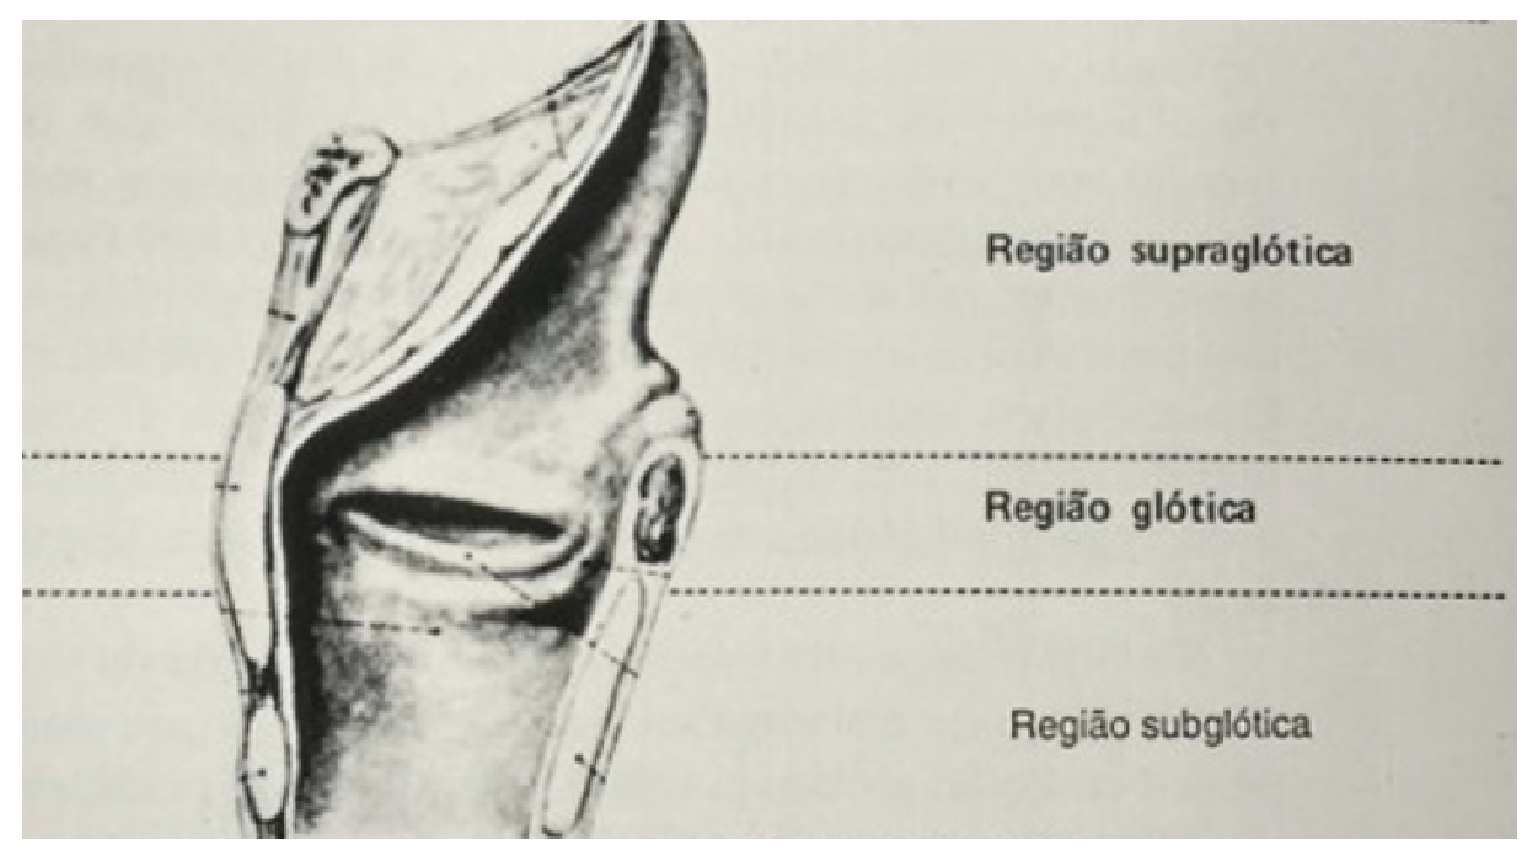
\includegraphics[width=300pt]{laringe_basico.eps}
\caption{Corte transversal de uma laringe, adaptado de \cite{livro_laringe_henrique}}
\label{fig:laringe_basico}
\end{figure}
\section{O Sinal de Voz}
\label{sec:sinal_voz}
\hspace*{+15pt} A voz \'{e} um sinal que, em sua origem n\~{a}o processada, \'{e} anal\'{o}gico. Isso significa que \'{e} poss\'{i}vel representar a voz em um gr\'{a}fico cujo os valores de abscissa representam um determinado instante no tempo. O problema \'{e} que, na sua ess\^{e}ncia, sinais anal\'{o}gicos cont\^{e}m infinitos valores dentro de um intervalo. É possivel ver na figura \ref{fig:onda_voz} um sinal de voz cujos valores de amplitude s\~{a}o utilizados para desenhar a onda ao longo de um determinado tempo.
\\
\par Esse problema conflita com a caracter\'{i}stica intr\'{i}nseca dos computadores de incapacidade de processar dados de tamanho infinito. Portanto, t\'{e}cnicas devem ser aplicadas para que um sinal anal\'{o}gico, no caso a voz, seja ent\~{a}o pass\'{i}vel de ser operado nos computadores. As t\'{e}cnicas aplicadas para a digitaliza\c{c}\~{a}o desse sinal, ou seja, para que esse sinal seja grande o suficiente de maneira que n\~{a}o perca suas caracter\'{i}sticas, mas que n\~{a}o seja infinitamente grande, ser\~{a}o discutidas na se\c{c}\~{a}o \ref{subsec:digitalizacao_voz}
\begin{figure}
\centering
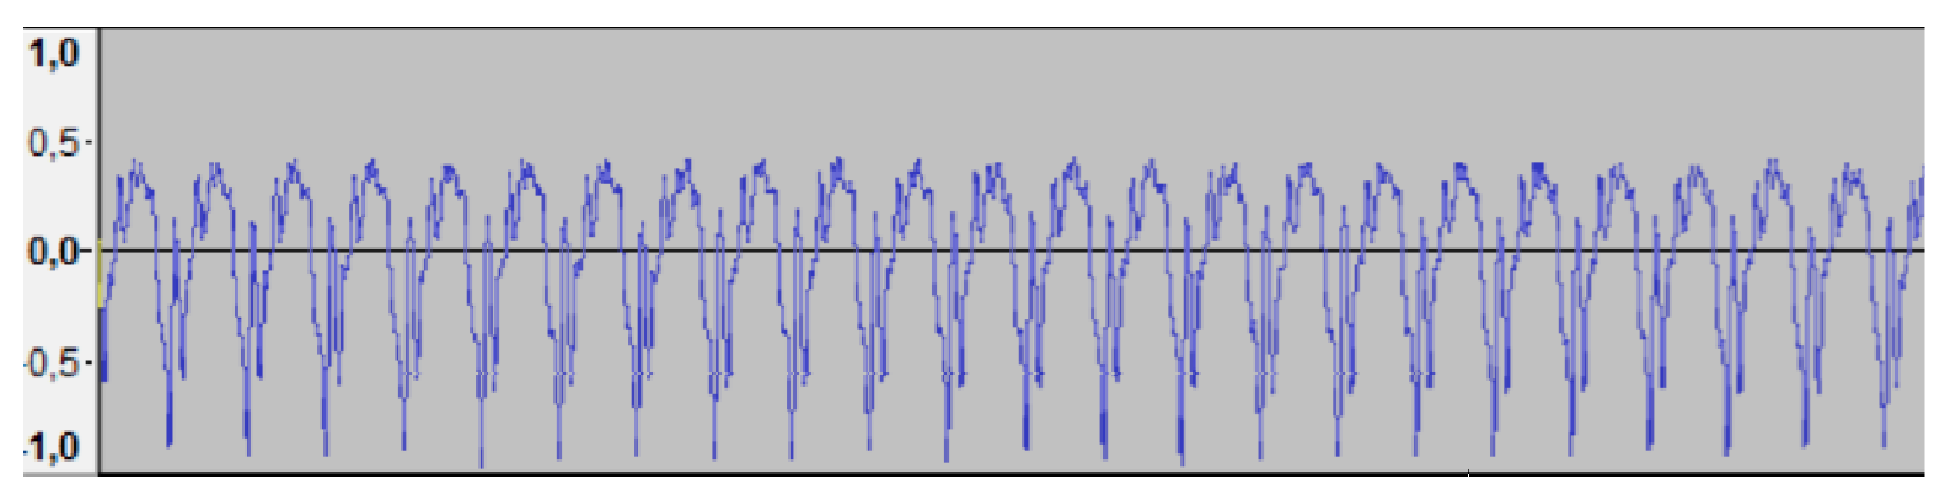
\includegraphics[width=350pt]{onda_voz}
\caption{Sinal de voz, visualizado no aplicativo \textit{Audacity}.}
\label{fig:onda_voz}
\end{figure}
\subsection{Digitaliza\c{c}\~{a}o do Sinal de Voz}
\label{subsec:digitalizacao_voz}
\par Como dito na se\c{c}\~{a}o \ref{sec:sinal_voz}, o sinal de voz precisa passar, antes de qualquer m\'{e}todo matem\'{a}tico, por m\'{e}todos para transfom\'{a}-lo em um sinal digital. Nessa se\c{c}\~{a}o, ser\'{a} discutido os dois processos pelo qual o sinal deve passar para poder ser considerado digital: discretiza\c{c}\~{a}o e quantiza\c{c}\~{a}o.
\\
\par Para discretizar o sinal, primeiro \'{e} necess\'{a}rio entender quantas amostras s\~{a}o necess\'{a}rias neste processo. A defini\c{c}\~{a}o \ref{shannon_nyquist_definition} mostra qual deve ser a taxa m\'{i}nima de amostragem que um sinal pode ter sem que perca suas caracter\'{i}sticas.
\begin{theorem_nyquist}
\label{shannon_nyquist_definition}
Considerando um sinal de frequ\^{e}ncia $B$, a quantidade de amostras por tempo, $f_s$, deve ser:
\null\hfill$f_s > 2B $\hfill \cite{definicao_taxa_amostragem1}\cite{definicao_taxa_amostragem2}
\end{theorem_nyquist}
\par Ap\'{o}s o processo de amostragem, o sinal agora pode ser representado por uma quantidade finita de pontos, definida pelo teorema\ref{shannon_nyquist_definition}. Por\'{e}m, os valores destes pontos ainda possuem infinitas casas decimais, ori\'{u}ndos da caracter\'{i}stica anal\'{o}gica do sinal. 
\\
\par Para sanar este problema, \'{e} aplicado o processo de quantiza\c{c}\~{a}o. Este processo consiste em dividir a amplitude do sinal analisado em v\'{a}rios intervalos de mesmo tamanho. Estes intervalos ser\~{a}o usados para auxiliar no arredondamento das amostras. Deve-se, amostra por amostra, arredondar o valor de uma amostra que tem muitas casas decimais para o limite inferior do intervalo em que a amostra est\'{a} contida.
\\
\par Feito isso, o sinal encontra-se digitalizado, e ent\~{a}o \'{e} capaz de ser processado por computadores digitais, e pode-se garantir que suas caracter\'{i}sticas foram preservadas.
\section{O Formato WAV}
\label{formato_wav}
\hspace*{+15pt} Um arquivo que esteja no formato \textit{.wav} obedece \`{a} uma estrutura particular que pode ser separa em dois campos: \emph{headers} e \emph{raw data}. Como \'{e} poss\'{i}vel ver na figura \ref{fig:wave_file}, o formato \'{e} divido em muitas outras categorias, entretanto o foco ser\'{a} o campo \emph{data}. Os outros campos possuem informa\c{C}\~{o}es gerais acerca do sinal digitalizado, conforme detalhado em \cite{formato_wave_completo}.
\\
\par O campo \emph{data} \'{e} fundamentalmente importante pois seus valores s\~{a}o importados para o programa, permitindo ent\~{a}o aplicar os m\'{e}todos matem\'{a}ticos da se\c{c}\~{a}o \ref{sec:extrator_caract}. Estes valores s\~{a}o n\'{u}meros inteiros que correspondem \`{a}s amplitudes digitalizadas. Assim, \'{e} preciso garantir que estes valores foram corretamente importados para o programa, pois qualquer erro nesta fase prejudicaria todo o processo aplicado, invalidando os resultados do projeto. 
\begin{figure}
\centering
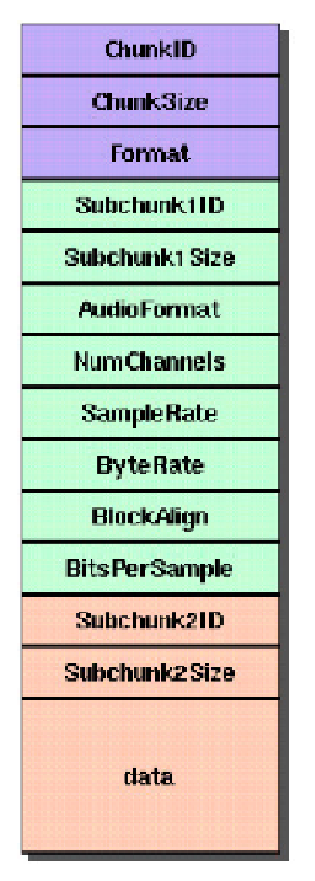
\includegraphics[width=80pt]{wave_file}
\caption{O formato de sinal \emph{wav}, retirado de \cite{figura_wave}.}
\label{fig:wave_file}
\end{figure}
\par Este formato armazena os dados em blocos (\emph{chunks}, na figura \ref{fig:wave_file}), e \'{e} uma varia\c{c}\~{a}o do formato RIFF. Um dos problemas, causados pelo uso de inteiros de 32 bits para gravar o tamanho do arquivo, \'{e} o tamanho m\'{a}ximo. Arquivos WAV n\~{a}o podem ultrapassar 4GB, por\'{e}m esta limita\c{c}\~{a}o n\~{a}o oferecer\'{a} problemas ao desenvolvimento do projeto, uma vez que os sinais duram em torno de 5 segundos. 
\\
\par Como \'{e} possivel ver na figura \ref{fig:wave_file}, o arquivo \'{e} dividido em um \emph{subchunk}, em tradu\c{c}\~{a}o livre sub-bloco, FMT e um \emph{subchunk} DATA. O sub-bloco FMT \'{e} o respons\'{a}vel por descrever o formato das informa\c{c}\~{o}es encontradas no sub-bloco DATA. Os campos da figura \ref{fig:wave_file} ser\~{a}o brevemente explicados: 
\begin{itemize}
\item \emph{ChunkID} Cont\'{e}m as letras RIFF em formato ASCII;
\item \emph{ChunkSize} \'{E} o tamanho de todo o arquivo em bytes, excluindo-se os 8 bytes dos campos n\~{a}o inclusos: ChunkID e ChunkSize;
\item \emph{Format} Cont\'{e}m as letras WAVE;
\item \emph{Subchunk1ID} Cont\'{e}m as letras \enquote{fmt}; 
\item \emph{Subchunk1Size} \'{E} o tamanho do resto do sub-bloco;
\item \emph{AudioFormat} Usado para mostrar se o sinal est\'{a} com alguma forma de compress\~{a}o de dados;
\item \emph{NumChannels} Define se o sinal \'{e} Mono, Stereo;
\item \emph{SampleRate} Taxa de amostras;
\item \emph{ByteRate} Este campo \'{e} definido pela f\'{o}rmula:  $(SampleRate * NumChannels * BitsPerSample)8$;
\item \emph{BlockAlign} N\'{u}mero de bytes, para uma amostra, incluindo todos os canais;
\item \emph{BitsPerSample} N\'{u}mero de bits que constitui cada amostra;
\item \emph{Subchunk2ID} Cont\'{e}m as letras \enquote{data};
\item \emph{Subchunk2Size} N\'{u}mero de bytes do campo \emph{data};
\item \emph{Data} Os valores brutos dos dados, e s\~{a}o os dados sobre os quais os m\'{e}todos ser\~{a}o aplicados.
\end{itemize}
\section{Extrator de Caracter\'{i}sticas}
\hspace*{+15pt} O extrator de caracter\'{i}sticas \'{e} uma ferramenta que ser\'{a} utilizada no projeto. Esta ferramenta consiste em receber uma grande quantidade de dados que podem ser informa\c{c}\~{o}es de diferentes origens, por exemplo, imagens e sinais ac\'{u}sticos. Neste projeto, as informa\c{c}\~{o}es providas ao extrator s\~{a}o os dados provenientes do campo Data, da figura \ref{fig:wave_file}. 
\\
\par A extra\c{c}\~{a}o \'{e} feita para que o classificador receba apenas uma quantidade reduzida de dados. Al\'{e}m de reduzir e fixar a quantidade das informa\c{c}\~{o}es , um aspecto importante da extra\c{c}\~{a}o de caracter\'{i}stica \'{e} a escolha da caracter\'{i}stica a ser extra\'{i}da. Diferentes caracter\'{i}sticas podem ser extra\'{i}das de um sinal ac\'{u}stico, e o extrator aqui constru\'{i}do ir\'{a} utilizar caracterist\'{i}cas energ\'{e}ticas. 
\\
\par Uma vez que o extrator de caracter\'{i}sticas encerra seu processo, todas as in\-for\-ma\-\c{c}\~{o}es que foram utilizadas como base para a produ\c{c}\~{a}o destas caracter\'{i}sticas podem ser desprezadas, uma vez que o classificador ir\'{a} operar diretamente nas informa\c{c}\~{o}es geradas pelo extrator. Desta maneira, o extrator, al\'{e}m de diminuir a quantidade de dados brutos e ser o meio no qual a extra\c{c}\~{a}o da caracter\'{i}stica escolhida \'{e} feito, tamb\'{e}m provê, ao classificador, todos os dados necess\'{a}rios para que o classificador possa atuar. 
\\
\par O processo de extra\c{c}\~{a}o \'{e} feito para que todos os sinais tenham uma caracter\'{i}stica em comum, que seja mensur\'{a}vel, e independente de fatores externos. Por exemplo, sinais podem ser gravados por homens e mulheres, e claramente têm muitas diferen\c{c}as. Por\'{e}m, aplicando-se um extrator, ambos os sinais podem ser comparados com uma mesma caracter\'{i}stica, seja ela qual for.  
\section{Classificador}
\hspace*{+15pt}Um classificador \'{e} uma das principais partes de um processo onde algo precise ser identificado, seja ele o estilo m\'{u}sica, o idioma. Desta maneira, o classificador tem como dados de entrada caracter\'{i}sticas extra\'{i}das no extrator, e sua sa\'{i}da \'{e} a classifica\c{c}\~{a}o daquilo que est\'{a} sendo testado. 
\\
\par Neste projeto, o classificador \'{e} a ferramenta respons\'{a}vel por classificar todos os sinais. Um classificador consiste de m\'{e}todos matem\'{a}ticos que ser\~{a}o aplicados aos valores providos pelo extrator de caracter\'{i}sticas. Neste processo, o classificador ir\'{a} comparar informa\c{c}\~{o}es entre os sinais que est\~{a}o sendo testados e aqueles que foram definidos como modelos. 
\\
\par Estes m\'{e}todos matem\'{a}ticos dependem diretamente da abordagem decidida. Diversas t\'{e}cnicas podem ser utilizadas, e entre as t\'{e}cnicas mais comuns, est\~{a}o dist\^{a}ncia Euclidiana e rede neurais. Tais t\'{e}cnicas s\~{a}o respons\'{a}veis por definir o que est\'{a} sendo analisado. Ou seja, em um programa cujo objetivo \'{e} discernir vozes saud\'{a}veis de patol\'{o}gicas, o classificador \'{e} o respons\'{a}vel pelo veredito: o sinal analisado \'{e} saud\'{a}vel ou patol\'{o}gico. 
\\
\par Ent\~{a}o, o classificador \'{e} constru\'{i}do no \^{a}mbito de identificar, ou classificar, o que est\'{a} sendo analisado pelo programa, e deve retornar um parecer. 
\section{Matriz de Confus\~{a}o}
\hspace*{+15pt} Uma matriz de confus\~{a}o \'{e} uma matriz quadr\'{a}tica, de ordem N, onde N \'{e} a quantidade de classes que o classificador pode escolher para aquilo que est\'{a} sendo testado. Esta matriz inicia preenchida de zeros.
\\
\par As linhas da matriz de confus\~{a}o s\~{a}o as classifica\c{c}\~{o}es originais, ou seja, as classifica\c{c}\~{o}es \`{a}s quais as informa\c{c}\~{o}es analisadas realmente pertencem. Quando a informa\c{c}\~{a}o que est\'{a} sendo testada pertence a uma certa classe, deve-se incrementar um a linha correspondente a mesma classe. 
\\
\par As colunas de uma matriz de confus\~{a}o representam a classifica\c{c}\~{a}o dada pelo programa. Ou seja, quando o classificador encerra, ele deve classificar a in\-for\-ma\-\c{c}\~{a}o testada em alguma das classes poss\'{i}veis. Cada linha representa uma classe, e quando o classificador decide a qual classe pertence aquela informa\c{c}\~{a}o, deve-se ent\~{a}o incrementar o valor da coluna correspondente a classe escolhida pelo classificador. 
\\
\par Desta forma, a diagonal principal desta matriz corresponde aos acertos do classificador, e \'{e} importante maximizar estes valores. As outras posi\c{c}\~{o}es na matriz s\~{a}o os erros, e, no caso de reconhecimento de patologias, estes erros podem ser classificados em 2 categorias: falso positivo e falso verdadeiro. 
\section{Valida\c{c}\~{a}o Cruzada}
\label{sec:validacao_cruzada}
\hspace*{+15pt} O processo de valida\c{c}\~{a}o cruzada \'{e} muito utilizado quando tempos dois grupos de informa\c{c}\~{a}o: modelos e testes. O processo de valida\c{c}\~{a}o cruzada consiste em embaralhar as informa\c{c}\~{o}es entre estes grupos. Quando um classificador come\c{c}a a executar, as informa\c{c}\~{o}es devem ser separadas em dois grupos, para que o classificador possa escolher um sinal dentre os testes, e compar\'{a}-lo com os sinais modelos. 
\\
\par Esta t\'{e}cnica contribui na fase de testes, uma vez que o teste de todas as possibildades pode ser invi\'{a}vel. Essa contribui\c{c}\~{a}o vem do fato que, quando as informa\c{c}\~{o}es s\~{a}o separadas, n\~{a}o se sabe qual \'{e} a melhor maneira de separ\'{a}-las. Portanto, separando aleat\'{o}riamente, tem-se um primeiro conjunto de informa\c{c}\~{o}es sobre o qual o classificador pode operar. 
\\
\par Ao final da classifica\c{c}\~{a}o, a utiliza\c{c}\~{a}o da valida\c{c}\~{a}o cruzada faz com que todos as informa\c{c}\~{o}es que ser\~{a}o utilizadas pelo classificador sejam misturadas, e ent\~{a}o sorteadas novamente, de maneira que o classificador opere em conjuntos de informa\c{c}\~{o}es diferentes. 
\\
\par Portanto, quando utiliza-se valida\c{c}\~{a}o cruzada, os grupos modelo e teste alteram frequentemente, em busca da melhor separa\c{c}\~{a}o poss\'{i}vel. A melhor divis\~{a}o pode ser encontrada de acordo com a quantidade de acertos feitos pelo classificador quando utilizado as informa\c{c}\~{o}es sorteadas. 
\\
\par A cada embaralhamento de informa\c{c}\~{o}es, novos conjuntos de dois grupos s\~{a}o formados, e os acertos e erros destes conjuntos devem ser comparados, de maneira a encontrar a melhor divis\~{a}o. 
%%%%%%%%%%%%%%%%%%%%%%%%%%%%%%%%%%%%%%%%%%%%%%%%%%%%%%%%%%%%%%
%%%%%%%%%%%%%%%%%%%%%%%%%%%%%%%%%%%%%%%%%%%%%%%%%%%%%%%%%%%%%%
%%%%%%%%%%%%%%%%%%%%%%%%%%%%%%%%%%%%%%%%%%%%%%%%%%%%%%%%%%%%%%
\chapter {O Sistema Proposto}
\emph{Neste Cap\'{i}tulo, o sistema proposto est\'{a} detalhado, em todos os seus passos. Sua leitura deve possibilitar compreender como o sistema foi estruturado e qual a id\'{e}ia principal por tr\'{a}s dele.}
\\
\par O sistema proposto neste trabalho possui os seguintes m\'{o}dulos que operam sequencialmente:
\begin{itemize}
\item{}m\'{o}dulo $M_1$: entrada de dados;
\item{}m\'{o}dulo $M_2$: extra\c{c}\~{a}o de caracter\'{i}sticas;
\item{}m\'{o}dulo $M_3$: classifica\c{c}\~{a}o;
\item{}m\'{o}dulo $M_4$: testes.
\end{itemize}
\par Particularmente com rela\c{c}\~{a}o ao m\'{o}dulo $M_1$, tomou-se o cuidado de, inicialmente, garantir que os valores digitalizados dos sinais WAVE estavam sendo importados corretamante. Assim, um breve procedimento de confer\^{e}ncia foi realizado: 
\begin{enumerate}
\item o sinal escolhido \'{e} exportado, por meio do aplicativo \textit{Audacity}, em um arquivo texto cujo conte\'{u}do est\'{a} representado nos campos da figura \ref{fig:wave_file};
\item o sinal escolhido \'{e} lido com a biblioteca de \textit{software} fornecida pelo orientador deste trabalho e os valores das amostras digitalizadas s\~{a}o impressos em um arquivo de texto. Apenas o \emph{raw data}, que corresponde ao campo \emph{data} da figura \ref{fig:wave_file}, \'{e} impresso.
\item os valores do arquivo em pleno texto gerado pelo \textit{Audacity} s\~{a}o comparados com aqueles obtidos com o uso da biblioteca, um a um, garantindo que s\~{a}o exatamente iguais.
\end{enumerate}
\par A t\'{i}tulo de exemplo, \'{e} possivel observar na figura \ref{fig:comparacao_ondas}-(a) e \ref{fig:comparacao_ondas}-(b), que as ondas geradas s\~{a}o perfeitamente iguais.
\begin{figure}[H]
\centering
\subfigure[Onda de voz gerada com os valores extra\'{i}dos pela biblioteca de \textit{software}]
{
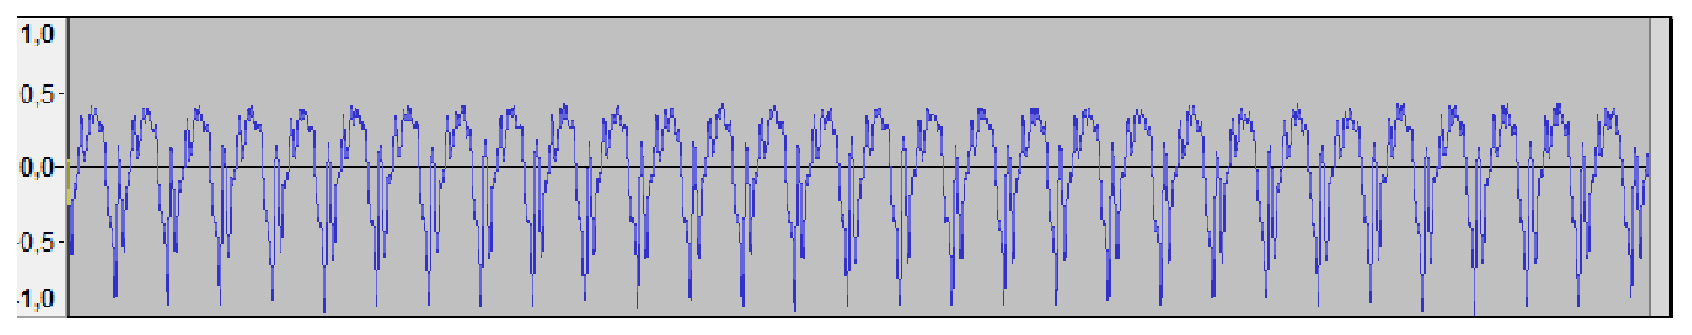
\includegraphics[width=450pt]{onda_voz_gerada.eps}
}
\subfigure[Onda de voz gerada no aplicativo \textit{Audacity}]
{
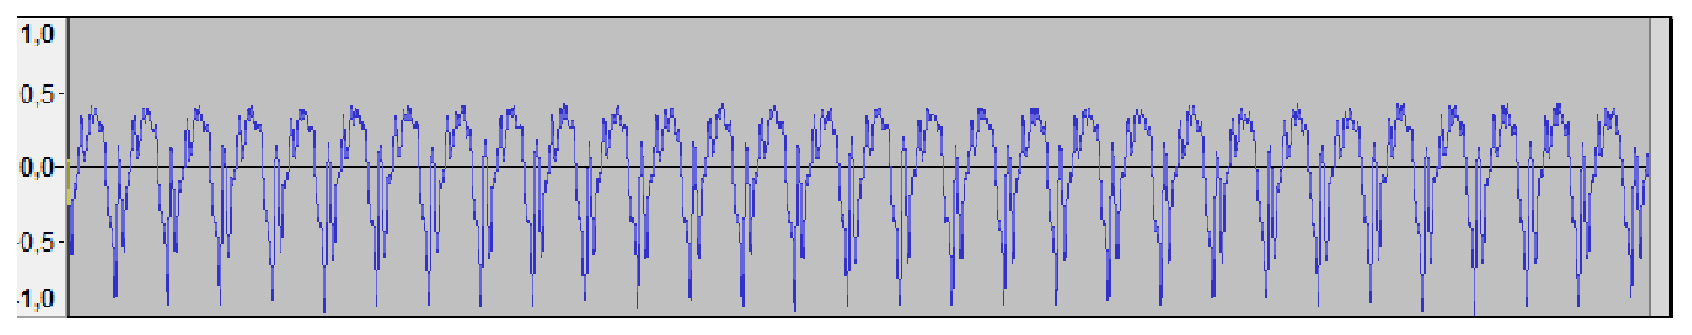
\includegraphics[width=450pt]{onda_voz_injetada.eps}
}
\caption{Ondas de voz}
\label{fig:comparacao_ondas}
\end{figure}
\par Uma vez que este processo garante a consist\^{e}ncia dos dados importados pela biblioteca utilizada, esta passou a ser acrescida de um consider\'{a}vel volume de c\'{o}digo-fonte em linguagem C/C++ desenvolvido por este autor, visando imlementar os m\'{o}dulos $M_2,M_3$ e $M_4$. 
\\
\par Com rela\c{c}\~{a}o ao m\'{o}dulo $M_2$, respons\'{a}vel pela  extra\c{c}\~{a}o de caracter\'{i}sticas, o objetivo \'{e} o de homogeneizar os sinais de voz de modo que eles sejam providos para o \emph{classificador} com a mesma quantidade de caracter\'{i}sticas. Assim, cada sinal de voz original, de tamanho consideravelmente alto e vari\'{a}vel, \'{e} convertido em sinais relativamente pequenos e de tamanhos fixos, chamados vetores de caracter\'{i}sticas. Al\'{e}m disso, tais vetores cont\'{e}m informa\c{c}\~{o}es \'{u}teis para a etapa classificadora.
\\
\par Particularmente, $M_2$ foi desenvolvido de modo a calcular a energia normalizada de cada janela de tamanho $P$ de cada sinal de voz, sobrepondo janelas consecutivas em $50\%$. Os valores de $P$ utilizados, em processos independentes, foram 256, 512, 1024, 2048, 4096. Nas situa\c{c}\~{o}es em que as amostras finais de um sinal de voz contivessem tamanhos insuficientes para caracterizar uma janela, o trecho final sofria um descarte. 
\\
\par Em seguida, todas as energias normalizadas foram convertidas em dois valores, apenas: \emph{m\'{e}dia} e \emph{vari\^{a}ncia}. Diante do exposto, cada um dos cinco valores de $P$ utilizados proporcionou uma m\'{e}dia e uma vari\^{a}ncia, implicando em um vetor de caracter\'{i}sticas de tamanho $10$. Resultados anteriores, contidos em textos referenciados na revis\~{a}o bibliogr\'{a}fica, trazem resultados documentando que a m\'{e}dia, e principalmente a vari\^{a}ncia, possuem potencial para indicar a presen\c{c}a de patologias em sinais de voz, justificando assim o uso de tais medidas estat\'{i}sticas. A presen\c{c}a de patologias na laringe, usualmente faz com que o locutor seja impedido de sustentar a const\^{a}ncia das caracter\'{i}sticas voc\'{a}licas necess\'{a}rias para caracterizar um padr\~{a}o normal de voz. Assim, vari\^{a}ncias consideravelmente altas nas energias dos sinais de voz indicam a presen\c{c}a de patologias. 
\\
\par Complementarmente, os dez valores contidos nos vetores de caracter\'{i}sticas foram armazenados em escala logar\'{i}tmica de modo a possuirem magnitudes suficientes para a visualiza\c{c}\~{a}o gr\'{a}fica confort\'{a}vel, vindo a auxiliar na observa\c{c}\~{a}o de padr\~{o}es, conforme as figuras \ref{fig:media_edema}, \ref{fig:media_nodulo}, \ref{fig:media_normal}, \ref{fig:variancia_edema}, \ref{fig:variancia_nodulo} e \ref{fig:variancia_normal}.
\begin{figure}[H]
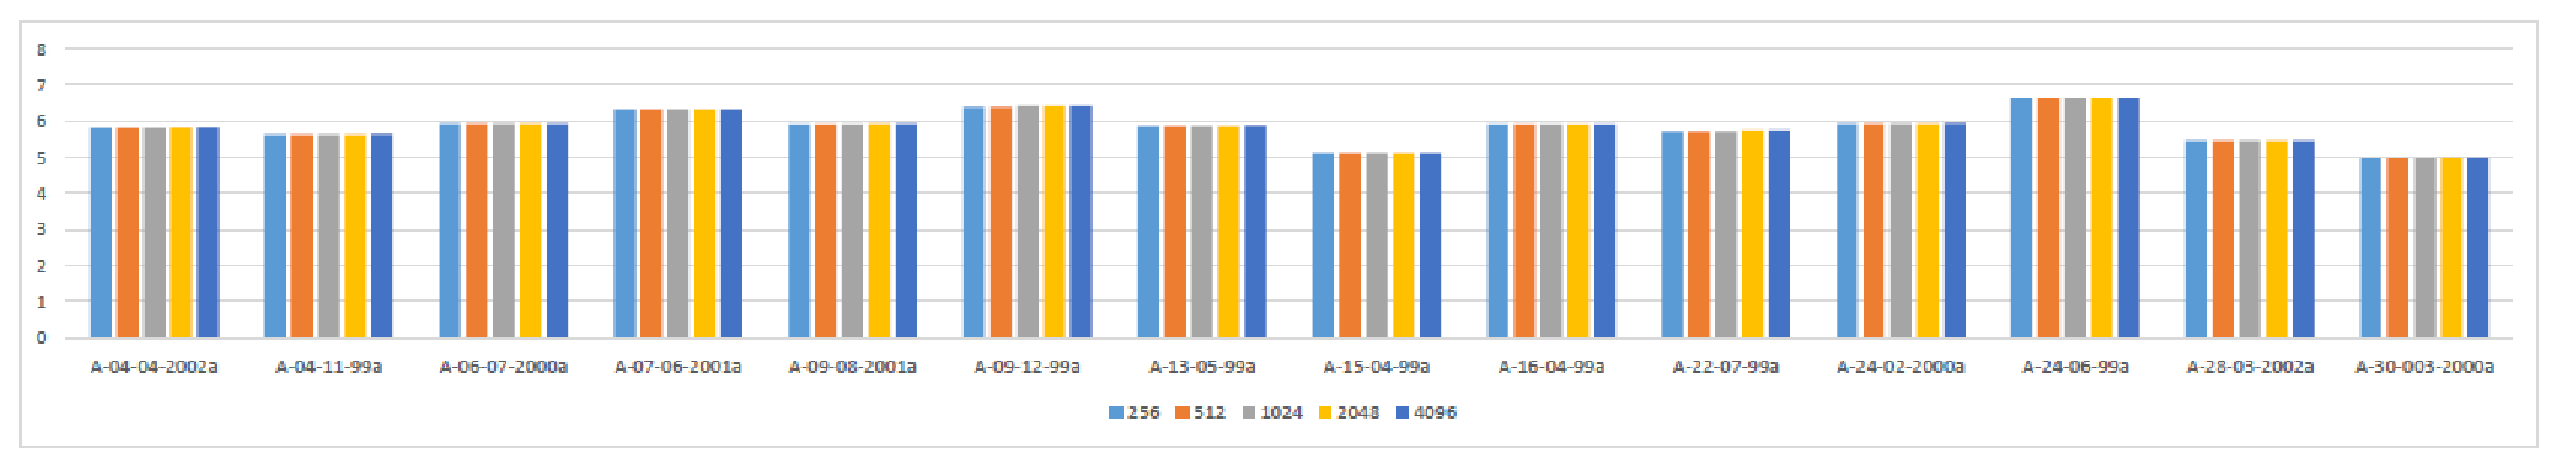
\includegraphics[width=1\textwidth, height=0.15\paperheight]{media_edema}
	\caption{Gr\'{a}fico de valores dos pacientes com edema, gerado atrav\'{e}s da m\'{e}\-dia pro\-ces\-sa\-da, agrupados por sinal, onde cada barra de uma certa cor corresponde a um tamanho de janela, de acordo com a legenda.}
	\label{fig:media_edema}
\end{figure}
\begin{figure}[H]
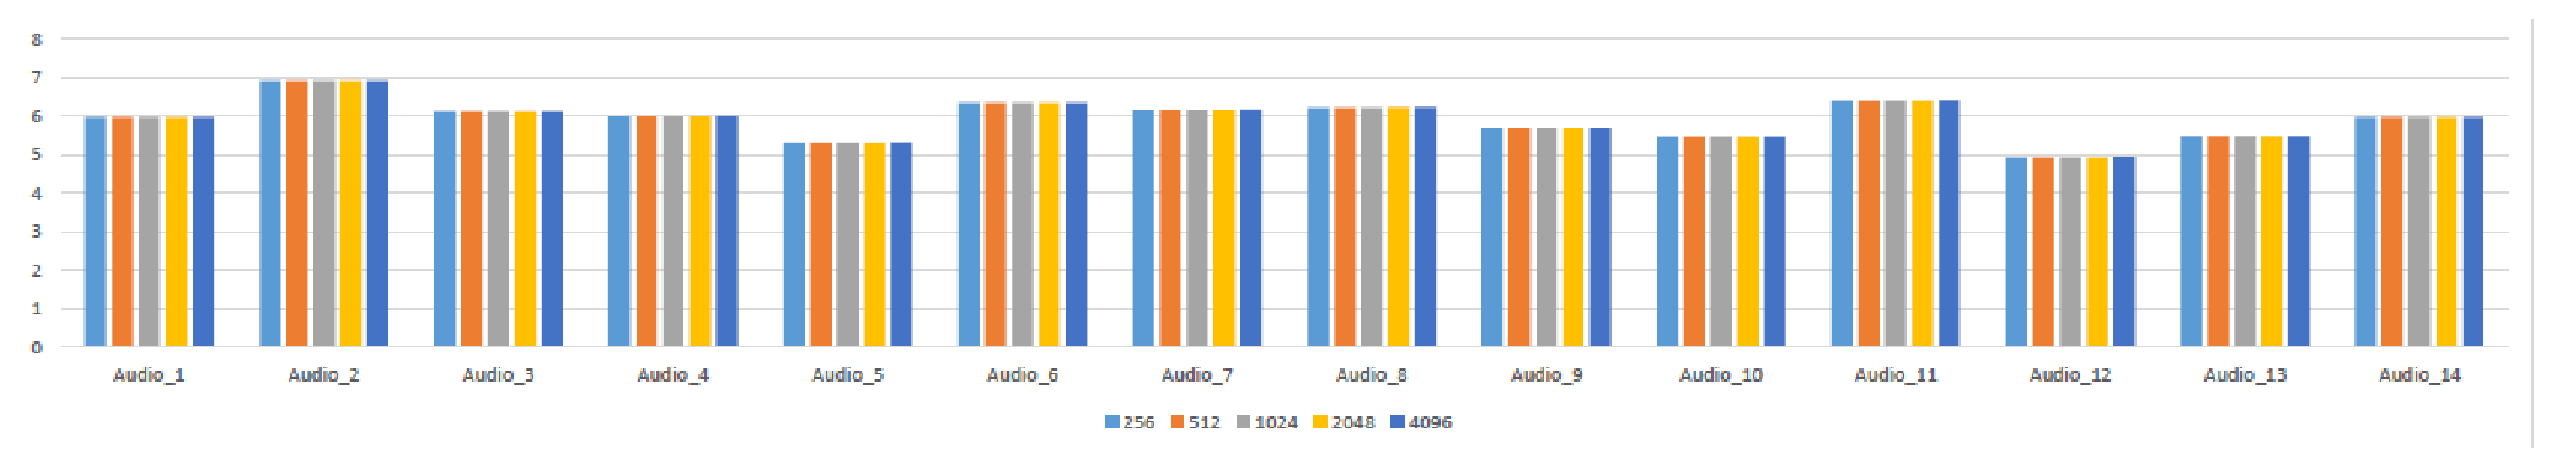
\includegraphics[width=1\textwidth, height=0.15\paperheight]{media_nodulo}
	\caption{Gr\'{a}fico de valores dos pacientes com n\'{o}dulo, gerado atrav\'{e}s da m\'{e}\-dia pro\-ces\-sa\-da, agrupados por sinal, onde cada barra de uma certa cor corresponde a um tamanho de janela, de acordo com a legenda.}
	\label{fig:media_nodulo}
\end{figure}
\begin{figure}[H]
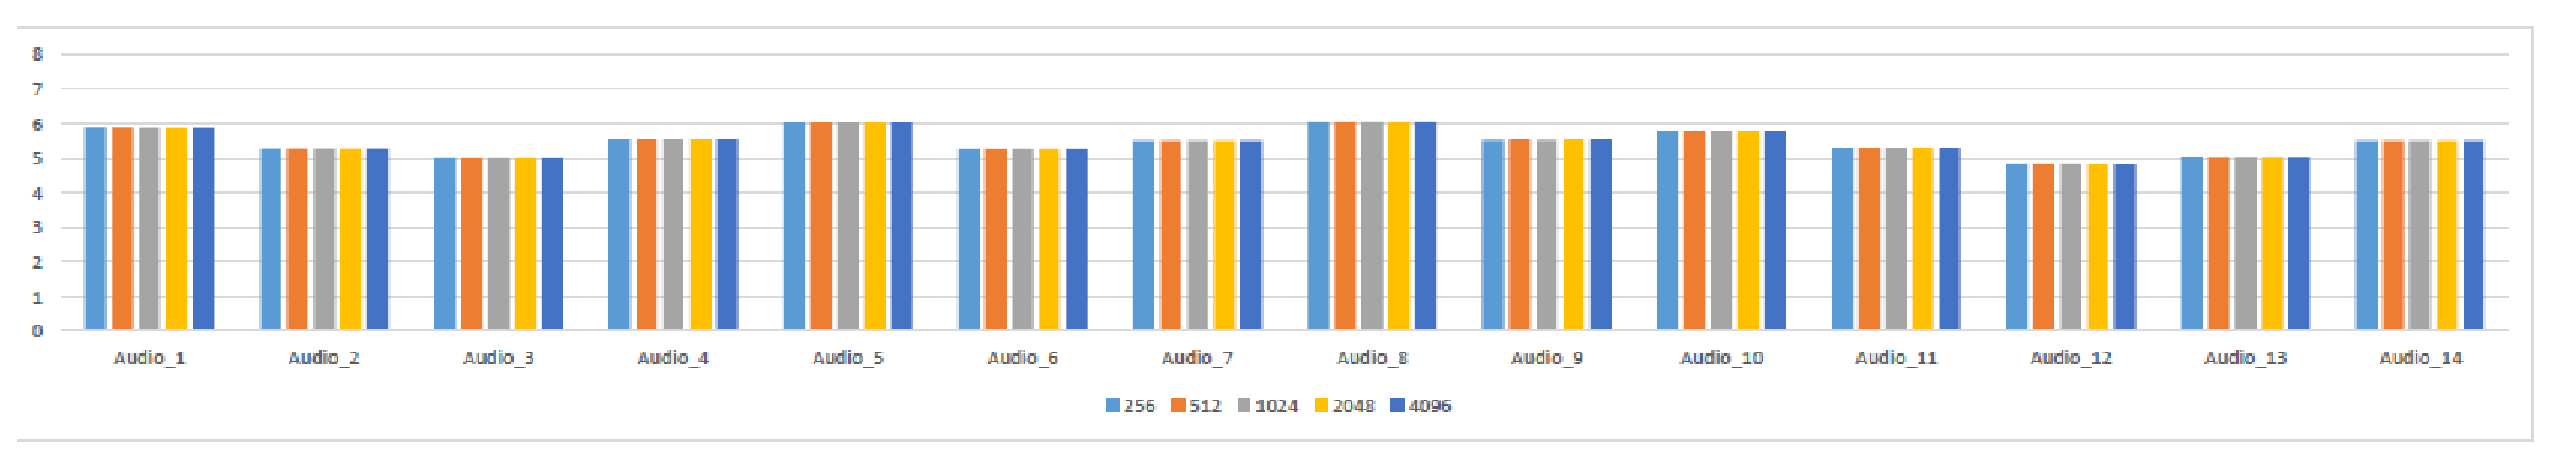
\includegraphics[width=1\textwidth, height=0.15\paperheight]{media_normal}
	\caption{Gr\'{a}fico de valores dos pacientes saud\'{a}veis, gerado atrav\'{e}s da m\'{e}\-dia pro\-ces\-sa\-da, agrupados por sinal, onde cada barra de uma certa cor corresponde a um tamanho de janela, de acordo com a legenda.}
	\label{fig:media_normal}
\end{figure}
\begin{figure}[H]
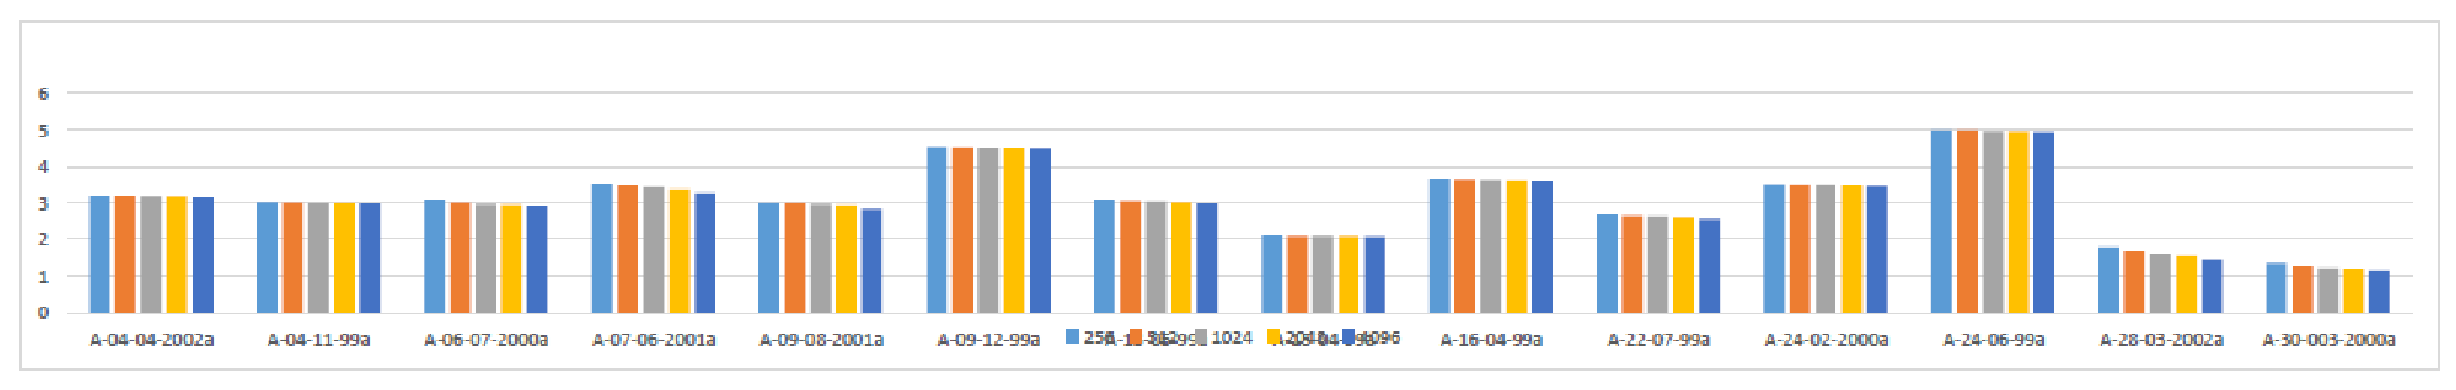
\includegraphics[width=1\textwidth, height=0.15\paperheight]{variancia_edema}
	\caption{Gr\'{a}fico de valores dos pacientes com edema, gerado atrav\'{e}s da va\-ri\-\^{a}n\-ci\-a processada, agrupados por sinal, onde cada barra de uma certa cor corresponde a um tamanho de janela, de acordo com a legenda.}
	\label{fig:variancia_edema}
\end{figure}
\begin{figure}
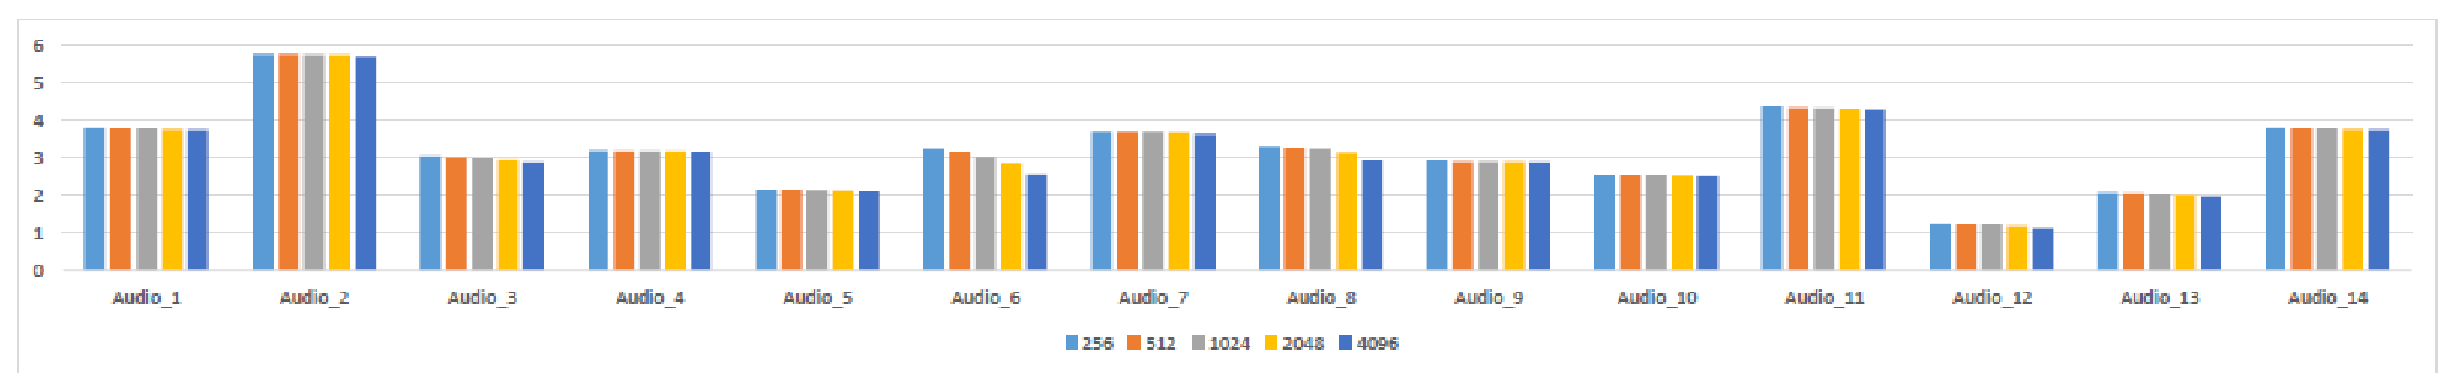
\includegraphics [width=1\textwidth, height=0.15\paperheight]{variancia_nodulo}
	\caption{Gr\'{a}fico de valores dos pacientes com n\'{o}dulo, gerado atrav\'{e}s da vari\^{a}ncia processada, agrupados por sinal, onde cada barra de uma certa cor corresponde a um tamanho de janela, de acordo com a legenda.}
	\label{fig:variancia_nodulo}
\end{figure}
\begin{figure}
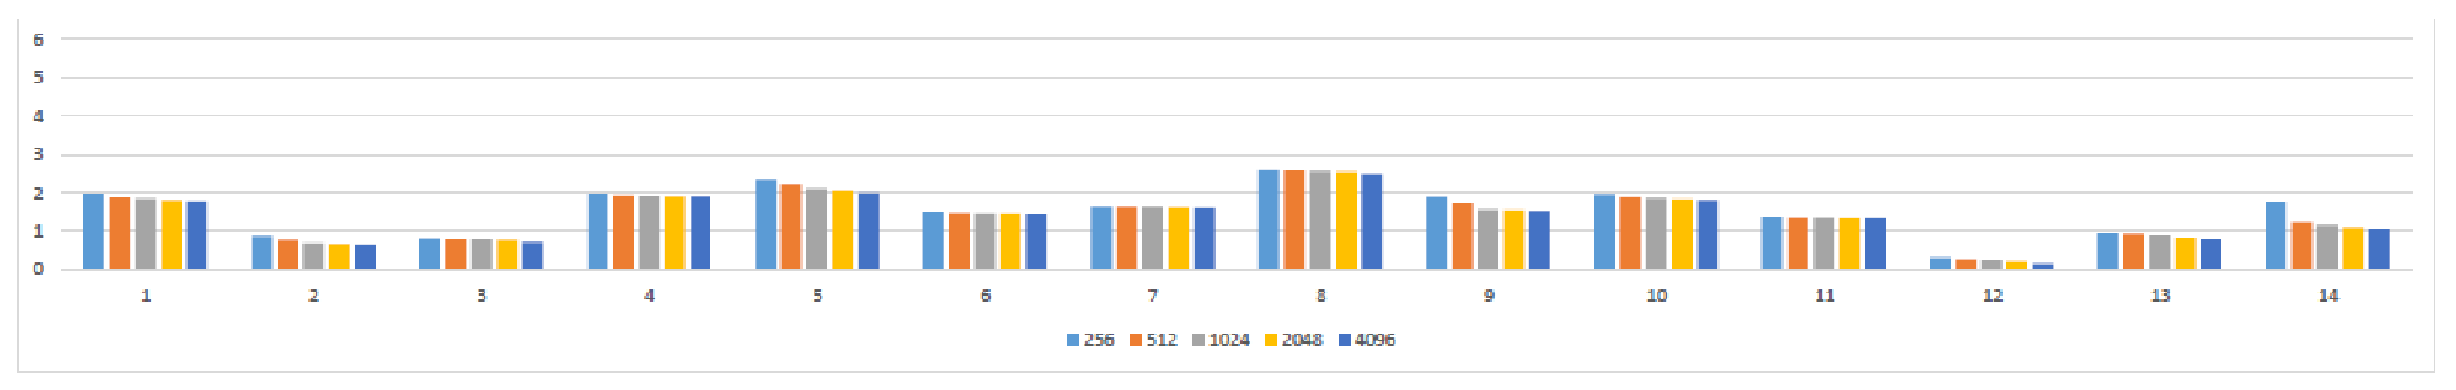
\includegraphics[width=1\textwidth, height=0.15\paperheight]{variancia_normal}
	\caption{Gr\'{a}fico de valores dos pacientes saud\'{a}veis, gerado atrav\'{e}s da va\-ri\-\^{a}n\-ci\-a processada, agrupados por sinal, onde cada barra de uma certa cor corresponde a um tamanho de janela, de acordo com a legenda.}	
	\label{fig:variancia_normal}
\end{figure}
\par Particularmente nas figuras \ref{fig:variancia_edema}, \ref{fig:variancia_nodulo} e \ref{fig:variancia_normal} \'{e} poss\'{i}vel observar os gr\'{a}ficos gerados com os valores de va\-ri\-\^{a}n\-ci\-a processados. Por\'{e}m, a an\'{a}lise visual possibilita uma conclus\~{a}o. Ao visualizar estes valores, \'{e} poss\'{i}vel ver na figura \ref{fig:variancia_normal} que os valores de vari\^{a}ncia dos pacientes saud\'{a}veis s\~{a}o significativamente menores que os valores de vari\^{a}ncia dos pacientes com edema, figura \ref{fig:variancia_edema}, e para os pacientes com n\'{o}dulo, \ref{fig:variancia_nodulo}. 
\\
\par Em seguida, passou-se a desenvolver o m\'{o}dulo $M_3$. Para ser poss\'{i}vel explicar o quesito de classifica\c{c}\~{a}o aplicado, primeiro deve-se ter em mente como os vetores ser\~{a}o agrupados. Dentre os 42 sinais, foram sorteados aleat\'{o}riamente 7 de cada classe e, ent\~{a}o, estes foram colocados no grupo \emph{modelo}. Este grupo consiste dos vetores aos quais os valores analisados ser\~{a}o comparados. Portanto, tem-se 21 vetores: 7 deles de pacientes com n\'{o}dulo, 7 com edema de Reinke e 7 saud\'{a}veis. Restaram ent\~{a}o 21 sinais, que foram agrupados no grupo \emph{teste}, que consiste dos vetores que ser\~{a}o testados.
\\
\par Uma das t\'{e}cnicas de classifica\c{c}\~{a}o que ser\'{a} aplicada \'{e} a Dist\^{a}ncia Euclidiana (DE) \cite{distancia_euclidiana}. Esta m\'{e}trica \'{e} uma medida utilizada para encontrar a dist\^{a}ncia entre dois pontos. Primeiramente, foi medida a DE de cada vetor sob teste em rela\c{c}\~{a}o a \emph{todos} os vetores do grupo modelo. Assim, deve ser encontrado o menor valor poss\'{i}vel, que indica a maior similaridade. Quando encontrado o menor valor, deve-se ent\~{a}o rotular o sinal que esta sendo testado como pertencente \`{a} mesma classe do sinal modelo cujo menor valor originou a menor DE. 
\\
\par Em outras palavras, a fase de teste consiste no seguinte algor\'{i}tmo:
\begin{enumerate}
\item escolher um vetor para teste, dentre os 21 sinais do grupo \emph{teste}.
\item encontrar a menor DE entre os valores deste vetor e \emph{todos} aqueles do grupo \emph{modelo}.
\item ao encontrar a menor DE, rotular o sinal respectivo: Edema, Nodulo ou Saud\'{a}vel.
\end{enumerate}
\par Cada classifica\c{c}\~{a}o executada neste algoritmo foi comparado a classifica\c{c}\~{a}o original do sinal de teste, gerando uma matriz de confus\~{a}o: se a classifica\c{c}\~{a}o do \textit{software} proposto for correta, deve-se acrescentar um ao valor da diagonal principal. Caso a classifica\c{c}\~{a}o esteja errada, deve-se incrementar um ao valor da linha correspondente. 
\\
\par O procedimento foi repetido para todos os sinais que se encontram no grupo de teste. Este processo faz surgir uma matriz de confus\~{a}o, onde \'{e} poss\'{i}vel analisar a quantidade de acertos e erros, globalmente. Cada matriz de confus\~{a}o\cite{referencia_matriz_confusao} utilizada para a verifica\c{c}\~{a}o possui ordem 3, cada uma correspondente ao grupo respectivo: normal, n\'{o}dulo e edema. Em princ\'{i}pio, o objetivo foi o de encontrar a matriz de confus\~{a}o cuja soma dos valores da diagonal principal seja o maior pos\-s\'{i}\-vel, garantindo a maior quantidade de acertos. 
\\
\par Observa-se que o procedimento de valida\c{c}\~{a}o cruzada foi aplicada com o objetivo de tentar encontrar a melhor matriz de confus\~{a}o poss\'{i}vel. Os sinais escolhidos e separados nos grupos foram aleatoriamente trocados, conforme detalhado adiante. Nota-se que, com a quantidade de sinais que foram utilizados, o processo de teste para todas as possibilidades de agrupamento dos sinais seria altamente dispendioso. Especificamente, os 42 sinais geram $\frac{14!}{7! (14-7)!}^3$ possibilidades de combina\c{c}\~{o}es, o que requereu um conjunto de testes aleat\'{o}rios em lugar da execu\c{c}\~{a}o de todas as possibilidades.
%%%%%%%%%%%%%%%%%%%%%%%%%%%%%%%%%%%%%%%%%%%%%%%%
%%%%%%%%%%%%%%%%%%%%%%%%%%%%%%%%%%%%%%%%%%%%%%%%
%%%%%%%%%%%%%%%%%%%%%%%%%%%%%%%%%%%%%%%%%%%%%%%%
\chapter{Testes e Resultados}
\label{chapter:tests}
\emph{Neste cap\'{i}tulo ser\~{a}o apresentados os processos empregados aos sinais. Estes processos foram aplicados, pro\-ven\-do ao clas\-si\-fi\-ca\-dor  os dados de entrada necess\'{a}rios para o pr\'{e}-diagn\'{o}stico dos pacientes analisados. Os testes feitos e suas abordagens, bem como os resultados dos mesmos, tamb\'{e}m s\~{a}o apresentados.}
\section{Base de Dados}
\hspace*{+15pt} Conforme mencionado anteriormente, a base de sinais que foi utilizada \'{e} composta de 42 sinais. Eles est\~{a}o dividos em 2 grandes grupos: patol\'{o}gicos e saud\'{a}veis. No grupo de sinais patol\'{o}gicos h\'{a} duas classifica\c{c}\~{o}es: pacientes com edema e pacientes com n\'{o}dulo. Cada um desses grupos \'{e} composto por 14 sinais. Ou seja, a base de sinais que foi utilizada para os testes cont\'{e}m dados de 14 pacientes saud\'{a}veis, 14 pacientes com n\'{o}dulo e 14 pacientes com edema. 
\\
\par Cada sinal consiste em um arquivo de formato WAVE. Em todos os 42 sinais, a locu\c{c}\~{a}o de cada paciente foi dura 5 segundos. Nesse per\'{i}odo de tempo, os pacientes sustentaram o som da vogal \emph{/a/}. Quando submetidos ao processo de amostragem a 22050 am/seg e de quantiza\c{c}\~{a}o com 16 bits, cada sinal gerou aproximadamente 130 mil valores para o extrator de caracter\'{i}sticas. 
\section{Procedimentos}
\hspace*{+15pt} Os procedimentos adotados neste trabalho podem ser divididos em duas fases: sor\-tei\-o dos vetores entre os grupos \emph{modelo} e \emph{teste} e classifica\c{c}\~{a}o de todos os sinais sorteados no grupo \emph{teste}. 
\\
\par A abordagem aleat\'{o}ria foi adotada para a separa\c{c}\~{a}o dos sinais porque, como visto anteriormente, seria impratic\'{a}vel testar todas as possibilidades. Portanto, para cada teste, os sinais foram divididos aleatoriamente entre os grupos de modelo e de teste. Os grupos \emph{modelo} e \emph{teste} foram compostos por 21 sinais cada, ou seja, a base de dados foi dividida em $50\%$ para modelos $50\%$ para testes. Desses 21 sinais, 7 eram pacientes saud\'{a}veis, 7 pacientes com n\'{o}dulos e 7 pacientes com edema. 
\\
\par Assim, a primeira fase de cada teste foi o sorteio dos sinais para a composi\c{c}\~{a}o do grupo de modelos. Dentre grupo de pacientes saud\'{a}veis foram sorteados aleatoriamente 7 pacientes, para que seus sinais compusessem o grupo modelo. Feito isso, os outros 7 sinais que n\~{a}o foram sorteados eram automaticamente colocados no grupo de testes. Este processo repetiu-se para os 14 pacientes com n\'{o}dulos e para os 14 pacientes com edemas, obedecendo ao mesmo crit\'{e}rio: os sorteados eram colocados como modelos, e n\~{a}o sorteados colocados como testes.  
\\
\par Ap\'{o}s a fase de sorteio, todos os dados estavam divididos entre os grupos modelo e teste, iniciando assim os testes. Nessa fase, cada sinal \'{e} representado por 10 valores de m\'{e}dias e vari\^{a}ncias processadas, providos pelo extrator de caracter\'{i}sticas, totalizando 210 valores (10 para cada sinal sorteado) no grupo \emph{modelo} e 210 valores no grupo \emph{teste}. 	
\\
\par Para que o processo de teste seja melhor explicado deve-se imaginar um sinal $X$ colocado no grupo de teste. Como dito anteriormente, esse sinal $X$ \'{e} representado por 10 valores gerados pelo processo de extra\c{c}\~{a}o de caracter\'{i}sticas. Cada um desses 10 valores do sinal $X$ foi comparado a todos os valores de todos os sinais no grupo \emph{teste}. Este processo consistiu na aplica\c{c}\~{a}o do crit\'{e}rio de DE. Durante os testes, cada vez que uma matriz de confus\~{a}o terminava de ser preenchida, ela era comparada a duas matrizes de confus\~{a}o: \emph{melhor matriz de confus\~{a}o} e a \emph{pior matriz de confus\~{a}o}, possibilitando redefinir quais foram os melhores e piores resultados. 
\\
\par A \emph{melhor matriz de confus\~{a}o} representa a melhor matriz encontrada. O crit\'{e}rio utilizado para a melhor matriz foi a soma da diagonal principal, ou seja, a soma de todos os acertos. A melhor matriz \'{e} substituida ao final de uma itera\c{c}\~{a}o se a soma da diagonal principal pertencente a matriz da itera\c{c}\~{a}o atual for maior que a soma da diagonal da melhor. Quando isso \'{e} feito, o algoritmo \'{e} capaz de informar exatamente quais os grupos de sinal estavam no grupo teste e no grupo modelo. 
\\
\par Isso foi feito para que, al\'{e}m de ser encontrada a melhor solu\c{c}\~{a}o, os vetores que geraram-na tamb\'{e}m fossem encontrados e analisados. Portanto a cada itera\c{c}\~{a}o obtia-se uma matriz de confus\~{a}o, e a ela comparava-se a melhor matriz, sendo substitu\'{i}da, se necess\'{a}rio. 
\\
\par O tratamento da melhor matriz repetiu-se no tratamento da pior matriz de confus\~{a}o. A cada nova matriz, obtida no final de uma itera\c{c}\~{a}o de classifica\c{c}\~{a}o, era executada uma compara\c{c}\~{a}o com a pior matriz. Por\'{e}m, o crit\'{e}rio utilizado para a substitui\c{c}\~{a}o foi a soma dos elementos que n\~{a}o pertenciam a diagonal principal. 
%//////////////////////////////////////////////////////////////////////////////////////////////
\section {Complexidade do Algoritmo}
\label{sec:complexidade}
\hspace*{+15pt} Devido a enorme quantidade de possibilidades para serem testadas, como visto anteriormente, cabe fazer uma an\'{a}lise da complexidade do algoritmo desenvolvido. Essa an\'{a}lise foi importante para a decis\~{a}o da quantidade de testes a serem executados. 
\\
\par O valor escolhido para a quantidade de testes deveria ser grande o suficiente para que os testes n\~{a}o representassem uma parte muito pequena do intervalo total, mas n\~{a}o t\~{a}o grande que o tempo de execu\c{c}\~{a}o fosse exagaredamente de\-mo\-ra\-do, tornando a execu\c{c}\~{a}o dos testes e a obten\c{c}\~{a}o dos resultados mais lenta que o necess\'{a}rio.
\\
\par Para isso, o algoritmo foi submetido a uma s\'{e}rie de testes. Esses testes consistiram em executar o programa com diferentes valores para a quantidade de itera\c{c}\~{o}es. Ao final do programa, seu tempo de execu\c{c}\~{a}o era exibido. Com diversas quantidades de testes, foi poss\'{i}vel a plotagem de um gr\'{a}fico, que pode ser visto na figura \ref{fig:tempo_exec}. 
\begin{figure}[H]
\centering
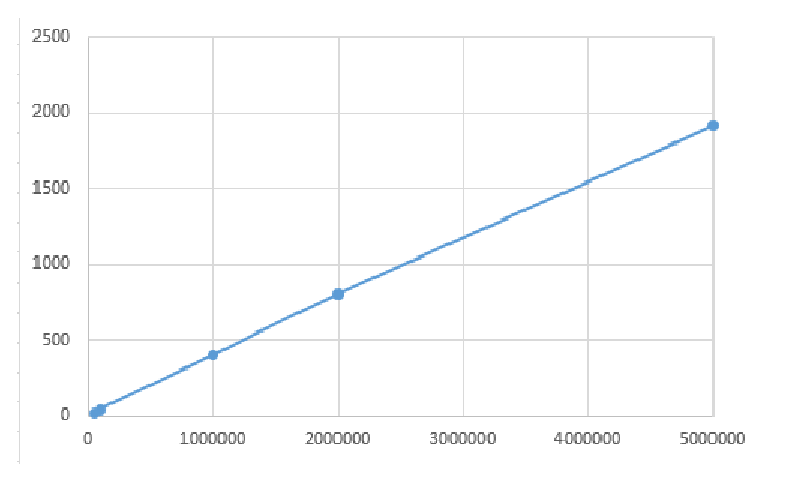
\includegraphics[width=400pt]{tempo_execucao.eps}
\caption{Gr\'{a}fico de tempo de execu\c{c}\~{a}o, no eixo $Y$, por tamanho da amostra, no eixo $X$. Percebe-se a rela\c{c}\~{a}o praticamente linear.}
\label{fig:tempo_exec}
\end{figure}
\par Na figura \ref{fig:tempo_exec} \'{e} poss\'{i}vel ver o tempo de execu\c{c}\~{a}o do algoritmo crescer conforme a amostra de testes aumenta. \'{E} poss\'{i}vel observar que a figura obtida \'{e} suficientemente pr\'{o}xima \`{a} uma reta. Essa an\'{a}lise emp\'{i}rica foi utilizada para comparar o tempo de execu\c{c}\~{a}o real do programa com o tempo de execu\c{c}\~{a}o previsto utilizando a complexidade do algoritmo obtida por meio dessa an\'{a}lise.
\\
\par Esse processo \'{e} importante para verificar a veracidade do tempo de execu\c{c}\~{a}o previsto, e, da mesma forma, embasar a decis\~{a}o da quantidade m\'{a}xima de testes executados, uma vez que essa decis\~{a}o est\'{a} fortemente ligada ao tempo de execu\c{c}\~{a}o para um valor escolhido. 
\\
\par Pela linearidade expl\'{i}cita na figura \ref{fig:tempo_exec}, os tempos previstos foram calculados usando propor\c{c}\~{a}o entre a quantidade de amostras anterior e o tempo de execu\c{c}\~{a}o da mesma. Os valores que deram origem a figura \ref{fig:tempo_exec}, bem como os valores previstos e o erro entre tempo de execu\c{c}\~{a}o previsto e tempo de execu\c{c}\~{a}o medido podem ser vistos na tabela \ref{tab:tabela_erro}. 
\begin{center}
\begin{table}[H]
    \begin{tabular}{ | l | l | l | p{1.8cm} |}
    \hline
    Quantidade de Testes & Tempo de Execu\c{c}\~{a}o & Tempo Esperado & Erro \\ \hline
    50000 & 19,317108 & - & - \\ \hline
    100000 & 39,600114 & - & - \\ \hline
    1000000 & 396,333647 & - & - \\\hline
    2000000 & 798,793876 & 792,667294 & 0,0076698 \\ \hline
    5000000 & 1909,128714 & 1996,98469 & -0,0460189 \\ \hline
    50000000 & 18987,98072 & 19091,28714 & -0,0054406\\ \hline
    \end{tabular}
\caption{Tamanhos dos vetores, tempos de execu\c{c}\~{a}o medidos, tempos de execu\c{c}\~{a}o obtidos atrav\'{e}s da complexidade do algoritmo e o erro entre o tempo esperado e o tempo obtido.}
\label{tab:tabela_erro}
\end{table}
\end{center}
\par Na tabela \ref{tab:tabela_erro}, a coluna \emph{Quantidade de Testes} representa quantos testes foram executados, a coluna \emph{Tempo de Execu\c{c}\~{a}o} representa o tempo medido, em segundos, da execu\c{c}\~{a}o da fun\c{c}~{a}o de classifica\c{c}\~{a}o dos sinais, a coluna \emph{Tempo Esperado} representa o tempo previsto de exe\-cu\-\c{c}\~{a}o, considerando uma complexidade linear. A coluna \emph{Erro} representa o \emph{Erro Relativo}\cite{calc_numerico} entre o tempo de execu\c{c}\~{a}o esperado e o tempo de execu\c{c}\~{a}o obtido. 
\\
\par Os valores na coluna \emph{Erro} n\~{a}o est\~{a}o representados em porcentagem. Ou seja, o valor $-0.0054406$ representa um erro de aproximadamente $0,5$\% do valor obtido em rela\c{c}\~{a}o ao valor previsto. Alguns valores na tabela \ref{tab:tabela_erro} s\~{a}o negativos pois o tempo gasto na execu\c{c}\~{a}o foi menor que o tempo previsto. 
\\
\par A complexidade do algoritmo apresentou valores suficientemente pr\'{o}ximos dos valores esperados, se considerado uma complexidade $\mathcal{O} (N)$, como pode ser visto na tabela \ref{tab:tabela_erro}. Comprovado a veracidade desses valores, a complexidade $\mathcal{O}(n)$ desempenhou um importante papel na decis\~{a}o da quantidade de testes. Como visto, a quantidade total de testes passa de \emph{40 bilh\~{o}es}. Portanto, para ser executado todos os testes poss\'{i}veis, em um processo \emph{single-threaded}, demoraria cerca de 185 dias para o final de exeu\c{c}\~{a}o. 
%\\\\\\\\\\\\\\\\\\\\\\\\\\\\\\\\\\\\\\\\\\\\\\\\\\\\\\\\\\\\\\\\\\\\\\\\\\\\\\\\\\\\\\\\\\\\\\
%//////////////////////// cod 8754 ///////////////////////////////////////////////////////////////////////
\section {Primeiros Resultados}
\label{sec:primeiros_resultados}
\hspace*{+15pt} Foram implementados, em linguagem C/C++, 400 milh\~{o}es de testes, buscando a melhor matriz de confus\~{a}o com base no processo explicitado na se\c{c}\~{a}o \ref{subsec:matriz_confusao}. Estes testes foram implementados com 4 \textit{threads}, designando 100 milh\~{o}es de testes para cada uma. 
\\
\par Cada \textit{thread} trabalhou de maneira independente, produzindo seus pr\'{o}prios arquivos. Isso foi feito para evitar qualquer tipo de problema de concorr\^{e}ncia e para tornar desnecess\'{a}ria a aplica\c{c}\~{a}o de algum mecanismo para controle de sincronismo (sem\'{a}foros, por exemplo). Com isso, o foco das \textit{threads} foi tornar o processo de teste mais r\'{a}pido, e de fato apresentou um tempo de teste aproximadamente quatro vezes mais r\'{a}pido que se um \'{u}nico programa fosse executado com 400 milh\~{o}es de testes. 
\subsection{Melhor Resultado}
\hspace*{15pt} Este resultado foi encontrado ap\'{o}s 400 milh\~{o}es de testes. A matriz de confu\~{a}o obtida ao final da execu\c{c}\~{a}o \'{e}:
$
\left(\begin{smallmatrix}
0 & 7 & 0 \\
3 & 4 & 0 \\
0 & 0 & 7 
\end{smallmatrix}\right)
$
\\
\par A matriz reflete um resultado preocupante: 3 classifica\c{c}\~{o}es do tipo  falso negativa. Para a classifica\c{c}\~{a}o entre \emph{saud\'{a}veis} e doentes, o resultado implicou em 52.38\% de acur\'{a}cia. Para o pr\'{e}-diagn\'{o}stico dos 7 pacientes com n\'{o}dulo, o algoritmo apresentou 57.14\% de precis\~{a}o. J\'{a} para a classifica\c{c}\~{a}o dos 7 pacientes com n\'{o}dulo, houve 100\% de acur\'{a}cia.
\\
\par O importante deste resultado \'{e} notar que os elementos definidos como falsos negativos implicaram que o algoritmo identificou um paciente doente como saud\'{a}vel. Esse problema foi levado em conta para o desenvolvimento de um crit\'{e}rio para refinar os resultados. 
\subsection{Pior Resultado}
\hspace*{15pt} O pior resultado, encontrado ao longo da execu\c{c}\~{a}o de 400 milh\~{o}es de testes est\'{a} representado pela matriz 
$
\left(\begin{smallmatrix}
7 & 0 & 0 \\
7 & 0 & 0 \\
7 & 0 & 0 
\end{smallmatrix}\right)
$
\\
\par Apesar de apresentar 100\% de precis\~{a}o para a classifica\c{c}\~{a}o dos 7 pacientes saud\'{a}veis, as categorias n\'{o}dulo e edema apresentaram 0\% de precis\~{a}o. E mais importante, para as duas categorias, todos os erros cometidos implicaram em falsos negativos. 
\\
\par Nesta execu\c{c}\~{a}o, o 	algoritmo ainda n\~{a}o apresentava crit\'{e}rios para decidir qual tipo de erro era mais danoso, entre falsos negativos e falsos positivos. Portanto, o fato de todos os erros terem sidos falsos negativos \'{e} uma consequ\^{e}ncia da aleatorieadade do programa. 
\\
\par A an\'{a}lise destas matrizes permite ver que os resultados encontrados podiam ser otimizados, de maneira que falsos negativos fossem evitados. O processo de otimiza\c{c}\~{a}o dos resultados obtidos, bem como os resultados propriamente otimizados, s\~{a}o discutidos adiante.
%\\\\\\\\\\\\\\\\\\\\\\\\\\\\\\\\\\\\\\\\\\\\\\\\\\\\\\\\\\\\\\\\\\\\\\\\\\\\\\\\\\\\\\\\\\\\\\\\\\\
\section {Otimiza\c{c}\~{a}o dos Resultados}
\subsection{Classifica\c{c}\~{a}o dos Erros}
\label{subsec:tipos_de_erro}
\hspace*{+15pt} Os erros cometidos pelo algoritmo proposto podem ser classificados em duas categorias: \emph{falsos positivos} e \emph{falsos negativos}. Essa distin\c{c}\~{a}o foi importante como crit\'{e}rio de desempate na compara\c{c}\~{a}o entre matrizes. 
\\
\par Um \emph{falso positivo} \'{e} uma classifica\c{c}\~{a}o, seja ela n\'{o}dulo ou edema, para a qual o paciente na verdade era saud\'{a}vel. Ou seja, um paciente saud\'{a}vel \'{e} sorteado para o teste e \'{e} classificado como patol\'{o}gico, independente da patologia erron\^{e}amente identificada. 
\\
\par O resultado desse pr\'{e}-diagn\'{o}stico pode levar o paciente a procurar um m\'{e}dico e submeter-se ao exame necess\'{a}rio, descobrindo ent\~{a}o que a classifica\c{c}\~{a}o dada pelo algoritmo havia sido incorreta. Essa situa\c{c}\~{a}o, por mais desagrad\'{a}vel, n\~{a}o o\-fe\-re\-ce risco a sa\'{u}de do paciente. 
\\
\par Apesar de, por v\'{a}rias vezes ao longo deste trabalho, ser explicado que o objetivo do mesmo \'{e} um \emph{pr\'{e}-diagn\'{o}stico}, um paciente diagnosticado como falso negativo \'{e} um s\'{e}rio problema. \emph {Falso negativo} significa que o programa classificou o paciente doente, esteja ele com n\'{o}dulo ou edema, como saud\'{a}vel. Isso pode levar o paciente a crer que est\'{a} bem, apesar de encontrar-se doente. 
\\
\par Para a minimiza\c{c}\~{a}o desse dano, o algoritmo foi programado de maneira que, quando um paciente pertence a classe doente e ele fosse classificado como saud\'{a}vel, esse erro tivesse um peso maior do que se fosse saud\'{a}vel e classificado como doente. Isso garante que a melhor e pior matriz levassem em conta os falsos positivos e falsos negativos. Na matriz de confus\~{a}o, o falso positivo \'{e} representado pelos elementos da segunda e terceira linha, ambos da primeira coluna. As figuras \ref{fig:falso_positivo} e \ref{fig:falso_negativo} exemplificam o caso. 
\\
\par Na figura \ref{fig:falso_positivo}, os elementos em vermelho representam os elementos de uma matriz de confus\~{a}o que equivalem a resultados falsos positivos.  J\'{a} na figura \ref{fig:falso_negativo}, os elementos em vermelho representam os resultados falsos negativos. 
%%%========== pedaco onde eh colocado as duas figuras das matrizes de falso positivo e falso negativo
\begin{figure}[H]
\centering

\includegraphics[width=180pt]{matriz_falso_positivo.eps}
\caption{matriz com erros falsos positivos.}
\label{fig:falso_positivo}
\end{figure}
\begin{figure}[H]
\centering

\includegraphics[width=150pt]{matriz_falso_negativo.eps}
\caption{matriz com erros falsos negativos}
\label{fig:falso_negativo}
\end{figure}
\par Devido a gravidade de resultados falsos negativos, foi gerado um crit\'{e}rio de desempate que considera falsos negativos piores que falsos positivos para encontrar a melhor matriz de confus\~{a}o. Foi aplicado um fator multiplicador aos elementos de falsos positivos e, da mesma maneira, um fator multiplicador foi aplicado aos elementos falsos negativos. 
\\
\par Isso garante que, quando em busca da melhor matriz de confus\~{a}o, o 	algoritmo evite considerar casos cujos resultados foram falsos negativos, fazendo com que os elementos, destacados em vermelho  na figura \ref{fig:falso_negativo}, fiquem o mais pr\'{o}ximo poss\'{i}vel de 0. 
\\
\par Os elementos da matriz de confus\~{a}o que n\~{a}o pertencem a diagonal principal e n\~{a}o est\~{a}o contemplados nas figuras \ref{fig:falso_positivo} e \ref{fig:falso_negativo} s\~{a}o diagn\'{o}sticos incorretos. Assim, o paciente realmente possu\'{i}a n\'{o}dulo e foi classificado como edema, ou o paciente possu\'{i}a edema e foi classificado como n\'{o}dulo. Estes 2 erros foram considerados equivalentes e, portanto, n\~{a}o foram utilizados como crit\'{e}rios de desempate. 
\\
\par Com essas observa\c{c}\~{o}es feitas, os testes foram executados novamente, e em maior escala. Utilizando todos os recursos de desempate descritos ao longo da se\c{c}\~{a} \ref{subsec:tipos_de_erro}, foram executados 800 milh\~{o}es de testes. O pior e melhor resultado, bem como suas matrizes de confus\~{a}o, ser\~{a}o discutidos a seguir. 
\section{Resultados Finais}
\hspace*{15pt} O pior resultado \'{e} aquele que cometeu maior quantidade de falsos negativos. Na matriz 
$
\left(\begin{smallmatrix}
0 & 7 & 0 \\
7 & 0 & 0 \\
7 & 0 & 0 
\end{smallmatrix}\right)
$
\'{e} poss\'{i}vel ver a quantidade de erros no pior resultado encontrado, implicando em 0\% de precisao em todas as classifica\c{c}\~{o}es. A primeira linha, que representa as classifica\c{c}\~{o}es dadas aos sinais de pessoas saud\'{a}veis, teve todos os sinais classificados como n\'{o}dulo. Como discutido anteriormente, esses erros n\~{a}o foram utilizados em crit\'{e}rios de desempate. Por\'{e}m, nas linhas seguintes da matriz de confus\~{a}o, \'{e} poss\'{i}vel ver que ambas patologias, n\'{o}dulo e edema, foram classificadas como normais, totalizando 14 falsos negativos. Esse resultado \'{e} claramente o pior poss\'{i}vel a ser obtido, uma vez que al\'{e}m de ter 0\% de precis\~{a}o, cometeu todos os erros graves possi\'{i}veis. 
\\
\par Tal resultado era esperado, devido ao forte peso atribu\'{i}do na soma dos erros quando um falso negativo era identificado. Assim, o algoritmo apresentou o comportamento esperado. 
\subsection{Melhor Resultado}
\hspace*{15pt} Ap\'{o}s a execu\c{c}\~{a}o dos 800 milh\~{o}es de testes, a melhor matriz de confus\~{a}o obtida foi 
$
\left(\begin{smallmatrix}
0 & 7 & 0 \\
0 & 6 & 1 \\
0 & 5 & 2 
\end{smallmatrix}\right)
$ .
\\
\par O crit\'{e}rio de desempate desenvolvido foi, assim, eficaz. Como pode ser visto na matriz, todos os erros considerados falso negativo foram extinguidos, cumprindo com o objetivo de minimizar a gravidade de erros que fossem cometidos.  Os sinais normais foram todos classificados como doentes com n\'{o}dulo, as este erro consiste em um falso positivo e, como dito anteriormente, n\~{a}o apresenta grave perigo a sa\'{u}de de um paciente. 
\\
\par Quanto a precis\~{a}o de classifica\c{c}\~{a}o entre saud\'{a}veis e patol\'{o}gicos, o algoritmo acertou 14 dos 21 sinais analisados, o que representa uma precis\~{a}o de 66,67\%. Essa precis\~{a}o foi medida considerando apenas dois tipos de sinais: saud\'{a}veis e doentes. 
\\
\par O 	algoritmo desenvolvido classificou corretamente todos os sinais patol\'{o}gicos como patol\'{o}gicos. Isso \'{e} de grande import\^{a}ncia, visto que nenhum paciente doente seria prejudicado por uma aus\^{e}ncia de diagn\'{o}stico. Dos 14 pacientes doentes, apenas 3 tiveram suas patologias classificadas erroneamente. De 7 pacientes com n\'{o}dulo, apenas um foi classificado como edema, e dentre os 7 pacientes com edema, 2 foram classificados com n\'{o}dulo. 
\\
\par Portanto, o algoritmo apresentou as seguintes precis\~{o}es: 66,67\% entre as clas\-si\-fi\-ca\-\c{c}\~{o}es saud\'{a}vel e patol\'{o}gico, 52,34\% se levado em considera\c{c}\~{a}o diagn\'{o}sticos errados entre os tipos de doen\c{c}a, 85,71\% para a classifica\c{c}\~{a}o de sinais com n\'{o}dulo, e 71,42\% para a classifica\c{c}\~{a}o de sinais com edema.
%%%%%%%%%%%%%%%%%%%%%%%%%%%%%%%%%%%%%%%%%%%%%%%%%%%%%%%%
%%%%%%%%%%%%%%%%%%%%%%%%%%%%%%%%%%%%%%%%%%%%%%%%%%%%%%%%
%%%%%%%%%%%%%%%%%%%%%%%%%%%%%%%%%%%%%%%%%%%%%%%%%%%%%%%%
\chapter{Conclus\~{o}es}
\hspace*{15pt} Este trabalho apresentou uma discuss\~{a}o, ainda que breve, sobre os problemas dos m\'{e}todos de diagn\'{o}sticos dispon\'{i}veis para a identifica\c{c}\~{a}o das patologias na laringe. Os m\'{e}todos s\~{a}o desconfort\'{a}veis para os pacientes, e isso foi um dos motivos que levou a cria\c{c}\~{a}o deste trabalho. Em seguida, foram apresentadas pesquisas sobre o reconhecimento n\~{a}o-invasivo de patologias na laringe. Al\'{e}m disso, todos os conceitos te\'{o}ricos abrangidos neste projeto foram exibidos tamb\'{e}m durante a fundamenta\c{c}\~{a}o te\'{o}rica.  
\\
\par No que tange ao algoritmo proposto, antes de aplica\c{c}\~{a}o de qualquer processamento, foi feita a digitaliza\c{c}\~{a}o dos sinais. Este processo obedeceu aos teoremas que o regem, como o Teorema da Amostragem. Prosseguindo,  o extrator de caracter\'{i}sticas constru\'{i}do foi aplicado a todos os sinais da base de dados. Ao final do extrator de caracter\'{i}sticas, 420 vetores de caracter\'{i}sticas de tamanho 10 foram providos ao classificador, que foi respons\'{a}vel por preencher a matriz de confus\~{a}o de acordo com seus acertos e erros. 
\\
\par O classificador, que empregou a Dist\^{a}ncia Euclidiana para classificar cada sinal colocado no grupo teste, obedeceu a um esquema de valida\c{c}\~{a}o cruzada, implicando em 1 bilh\~{a}o e 200 milh\~{o}es de sorteios, um sorteio para cada itera\c{c}\~{a}o de teste executada. 
\\ 
\par Ao longo dos testes, as matrizes de confus\~{a}o foram discutidas com o intuito de comprovar que, sem o crit\'{e}rio de desempate explanado, o 	algoritmo cometia erros graves e que podiam ser refinados para que o resultado do mesmo fosse o melhor o poss\'{i}vel. 
\\
\par Por fim, foram mostradas a melhor e a pior matriz de confus\~{a}o geradas. Na pior matriz, foi poss\'{i}vel observar que o crit\'{e}rio de desempate solucionou o problema de falsos negativos. Particularmente, na melhor matriz de confus\~{a}o obtida, o resultado foi de 66,67\% entre as clas\-si\-fi\-ca\-\c{c}\~{o}es saud\'{a}vel e patol\'{o}gico. Neste resultado, apenas 3 pacientes tiveram suas patologias confundidas pelo algoritmo, mas ainda assim eles foram classificados como oriundos de indiv\'{i}duos doentes. Para os 14 sinais patol\'{o}gicos, o 	algoritmo apresentou 100\% de precis\~{a}o, ou seja, nenhum paciente doente foi classificado como normal. Desse modo, satisfeitas est\~{a}o as expectativas.
\newpage
\begin{appendices}
\chapter{Valores gerados pelo programa} 
\hspace*{+15pt}Os sinais nesta se\c{c}\~{a}o, em vez de serem compostos por 10 valores como utilizado ao longo deste trabalho, ser\~{a}o representados por apenas dois valores: um que representa a m\'{e}dia de todas as m\'{e}dias processadas do sinal, representado em todas as figuras pela coluna azul, e um que representa a m\'{e}dia de todas as vari\^{a}ncias do sinal, representado em todas as figuras desta se\c{c}\~{a}o pela coluna laranja. 
\\
\par Isso foi feito na tentativa de transformar os gr\'{a}ficos para que fossem mais f\'{a}ceis de serem visualizados. Este processo n\~{a}o apresentou perda significativa das caraceter\'{i}sticas dos valores. Todas as 5 m\'{e}dias processadas e 5 vari\^{a}ncias processadas, ao serem transformadas em uma m\'{e}dia de m\'{e}dias processadas e uma m\'{e}dia de vari\^{a}ncias processadas tiveram seus desvios-padr\~{a}o medidos, e todas as amostras encontravam-se dentro do desvio. 
\begin{sidewaysfigure}
\centering
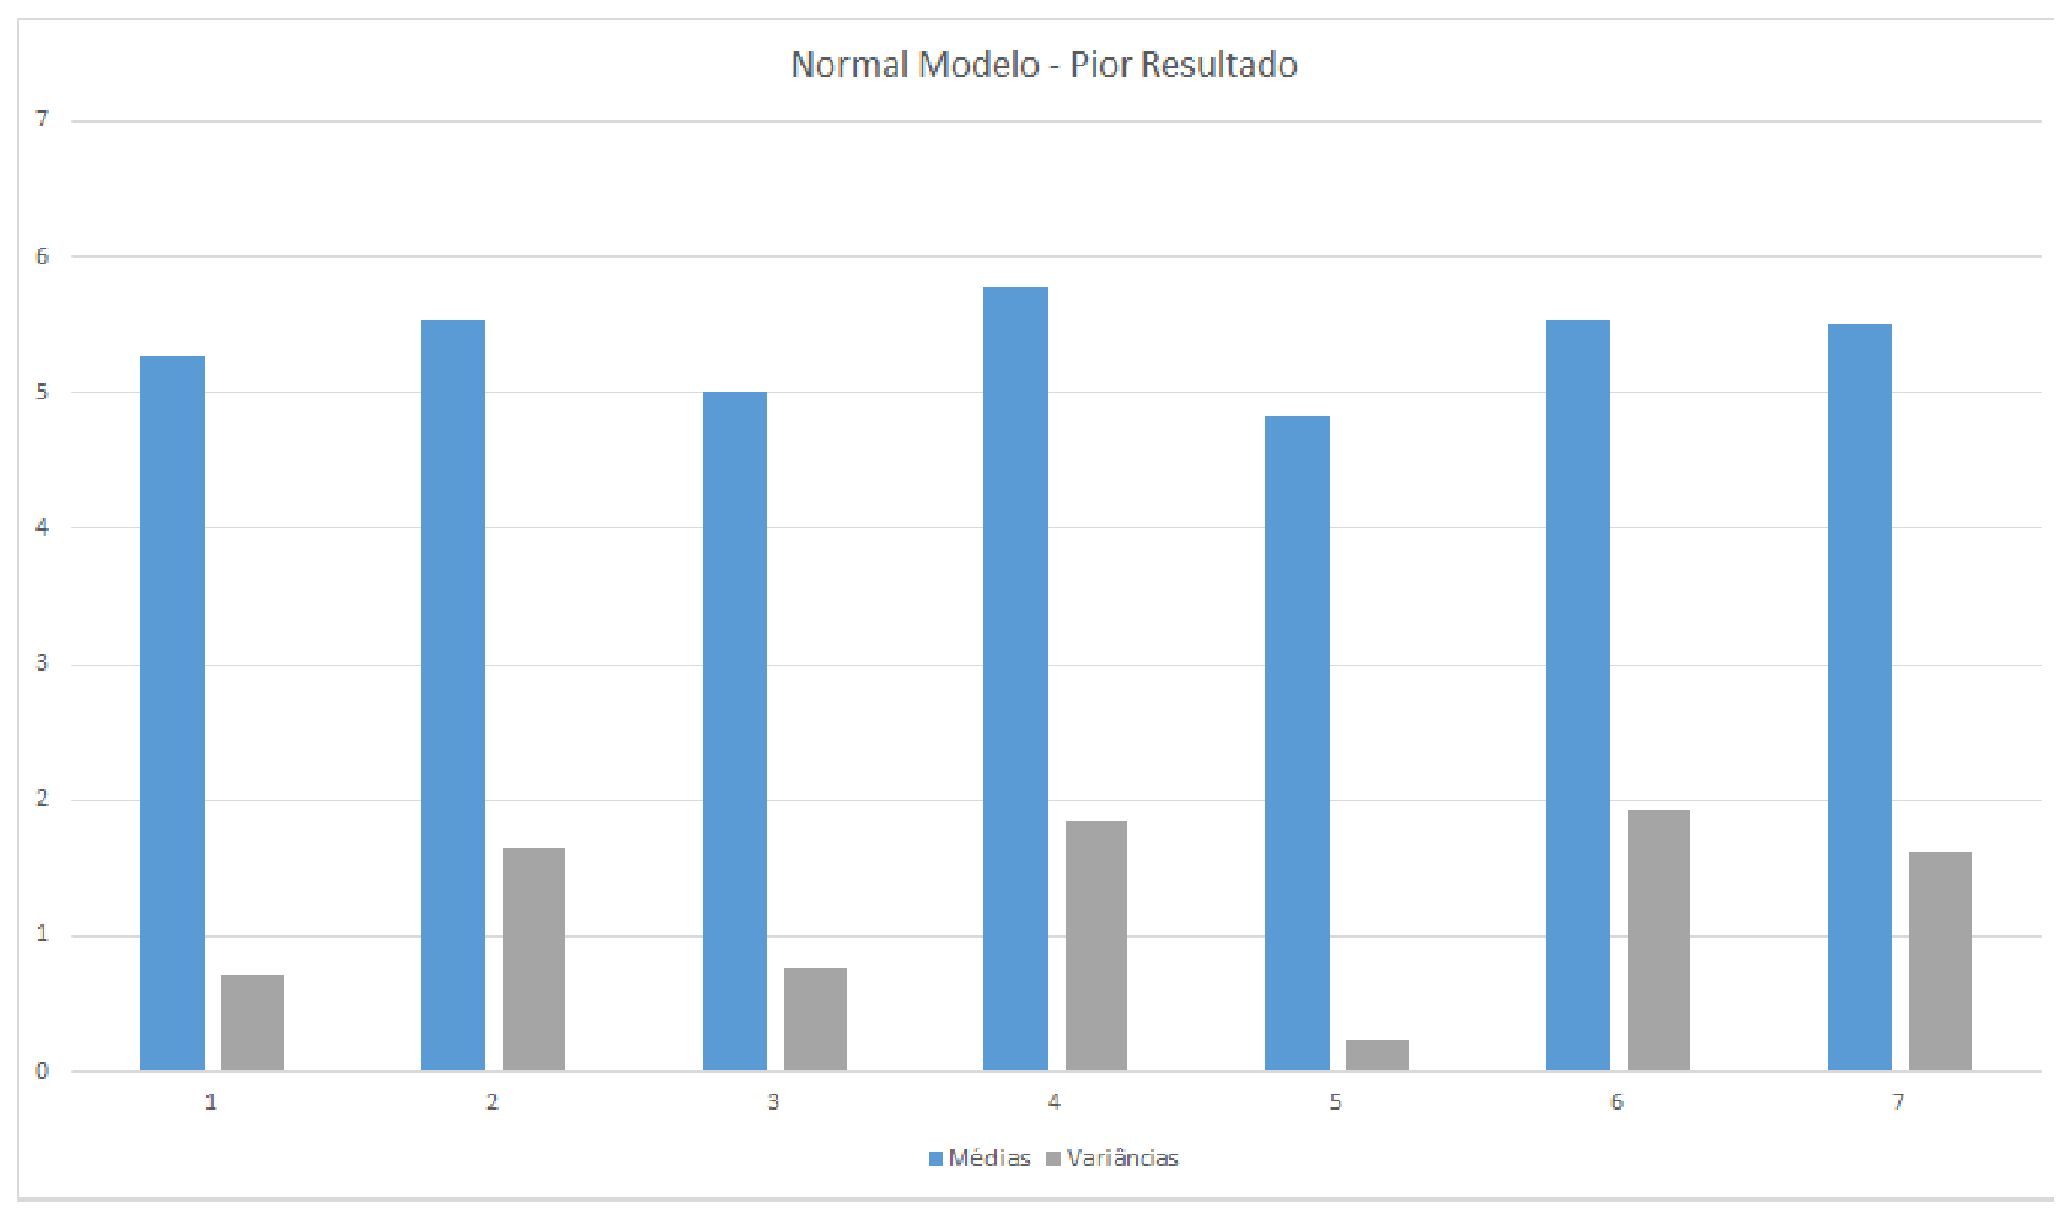
\includegraphics[width=0.70\hsize]{figuras_tcc/pior_resultado/normal_modelo_pior.eps}
\caption{Valores dos sinais saud\'{a}veis, selecionados para o grupo modelo, que geraram o pior resultado}
\label{fig:normal_modelo_pior}
\end{sidewaysfigure}
\begin{sidewaysfigure}
\centering
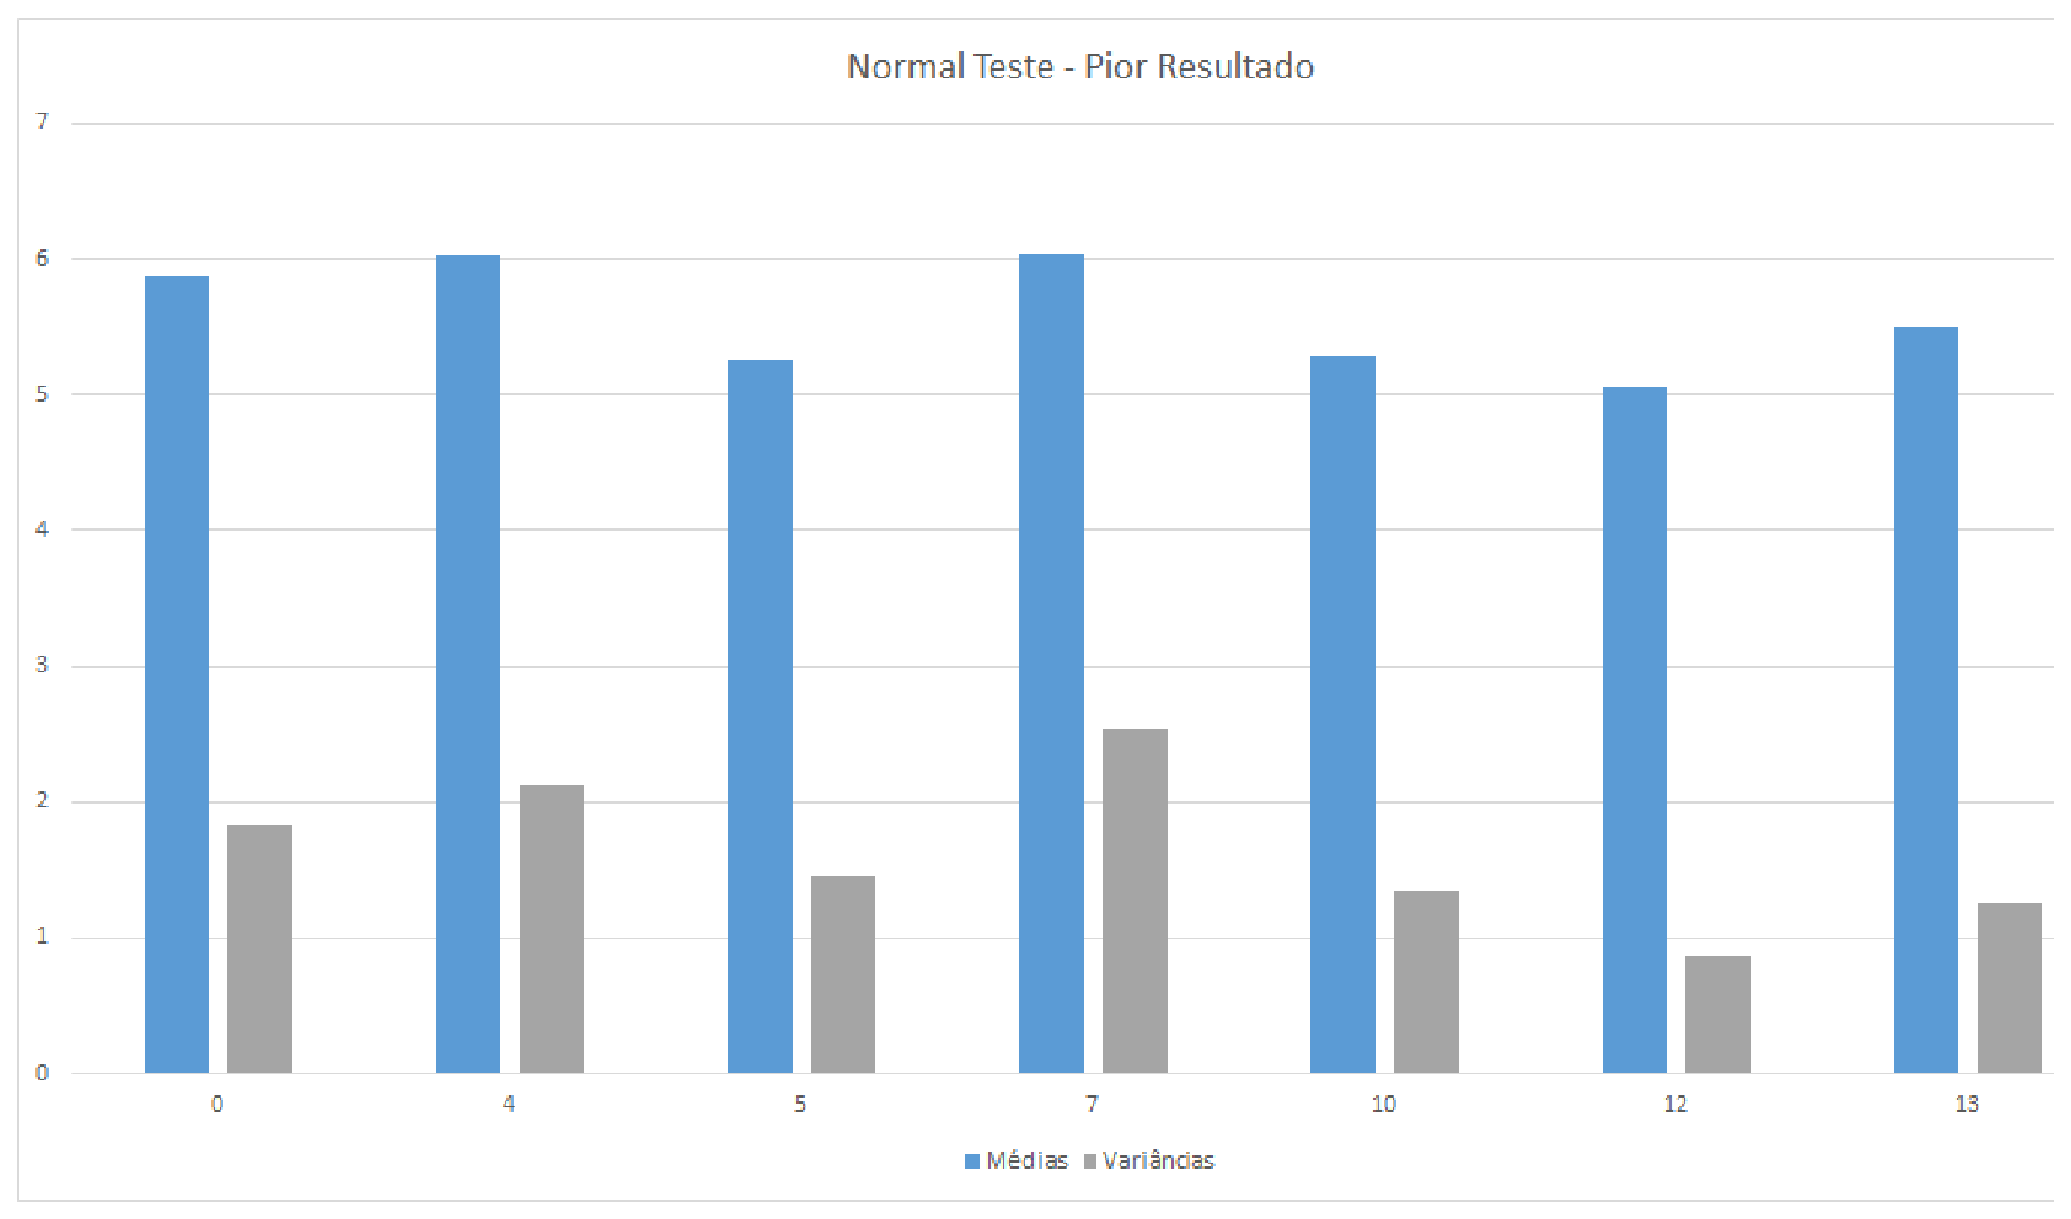
\includegraphics[width=0.70\hsize]{figuras_tcc/pior_resultado/normal_teste_pior.eps}
\caption{Valores dos sinais saud\'{a}veis, selecionados para o grupo teste, que geraram o pior resultado. }
\label{fig:normal_teste_pior}
\end{sidewaysfigure}
\begin{sidewaysfigure}
\centering
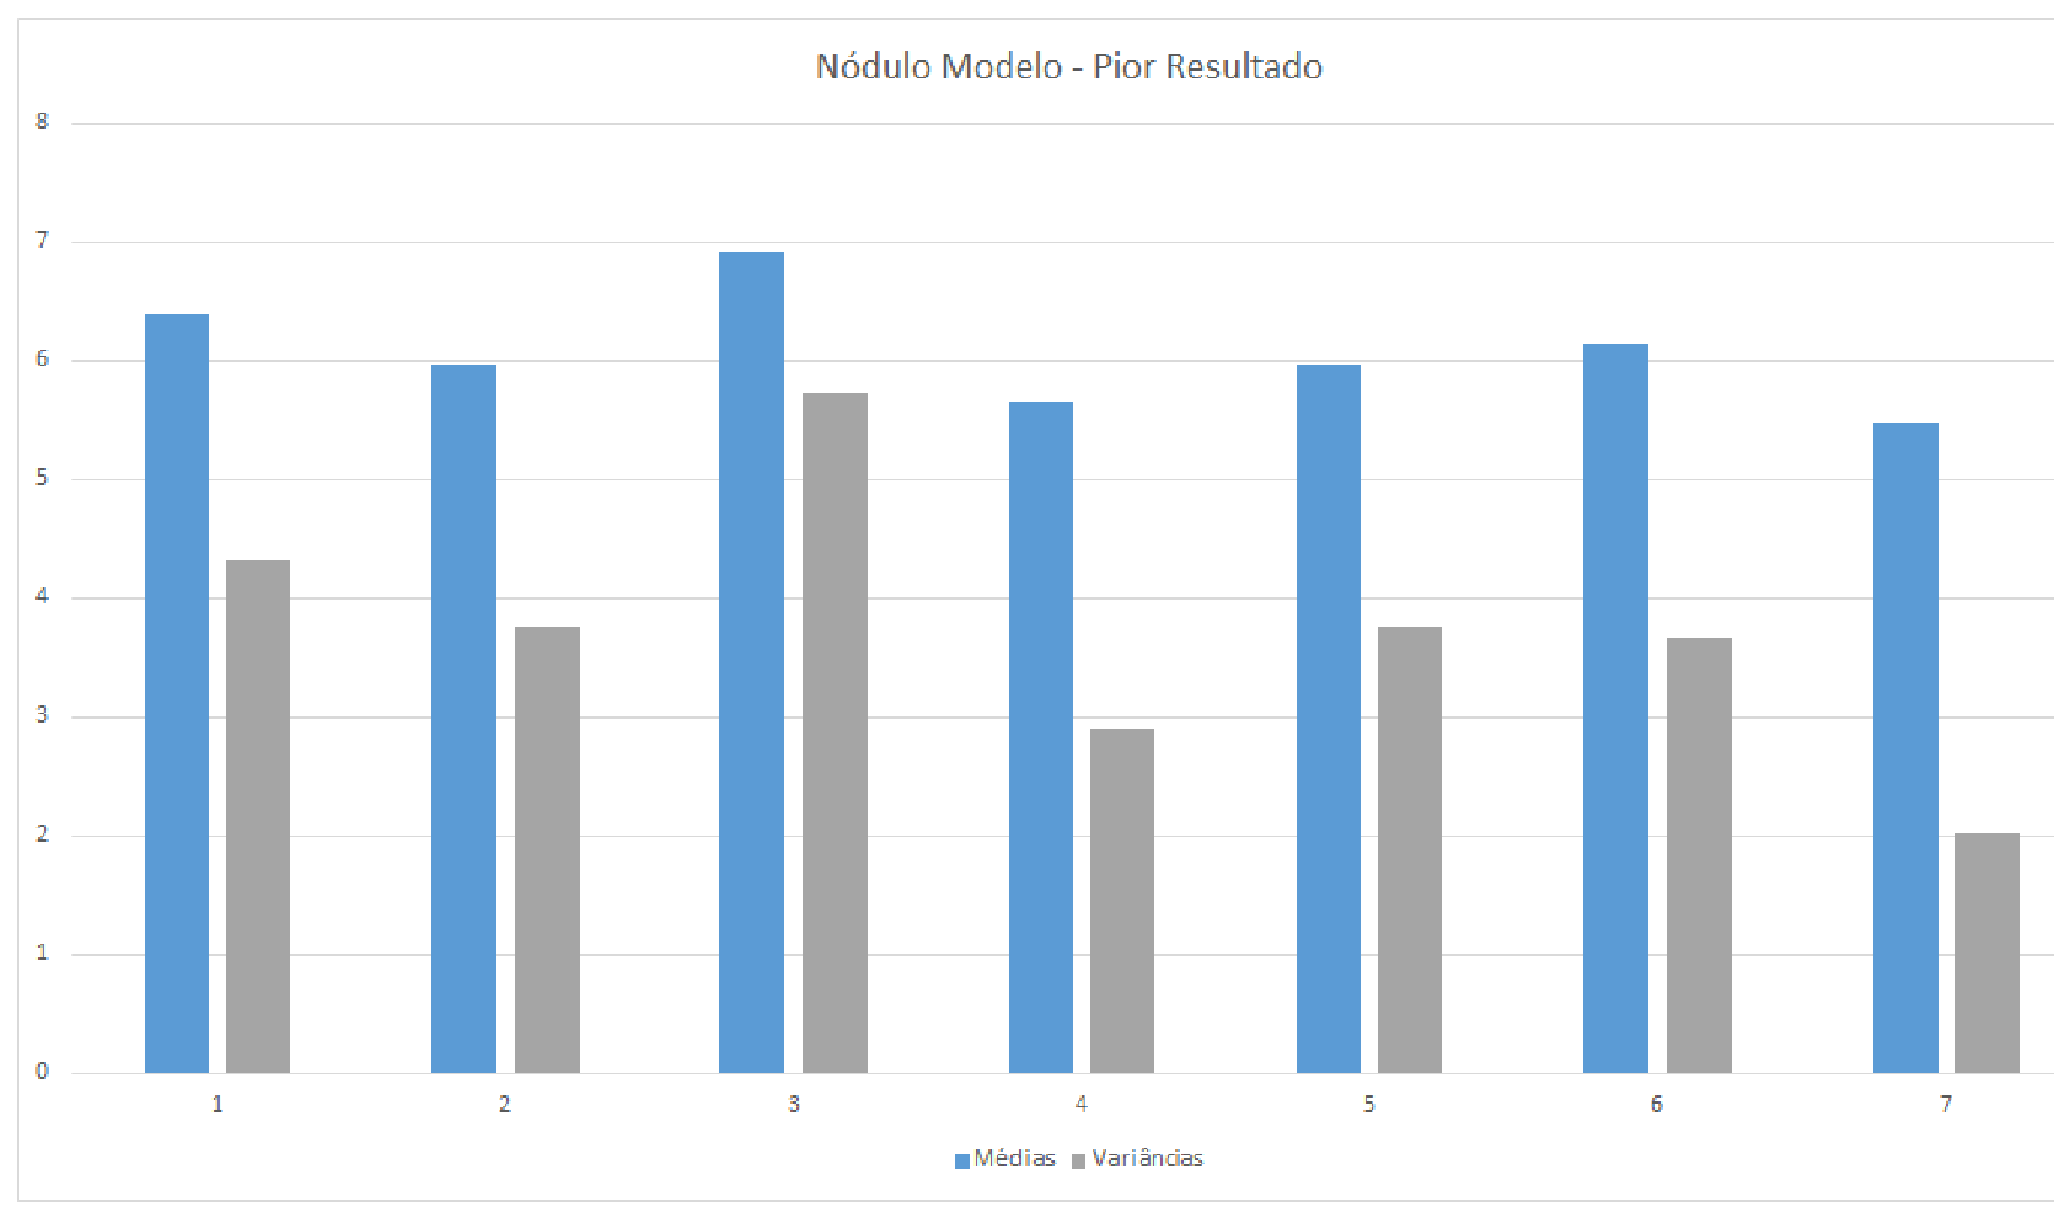
\includegraphics[width=0.70\hsize]{figuras_tcc/pior_resultado/nodulo_modelo_pior.eps}
\caption{Valores dos sinais de pacientes com n\'{o}dulo, selecionados para o grupo modelo, que geraram o pior resultado.}
\label{fig:nodulo_modelo_pior}
\end{sidewaysfigure}
\begin{sidewaysfigure}
\centering
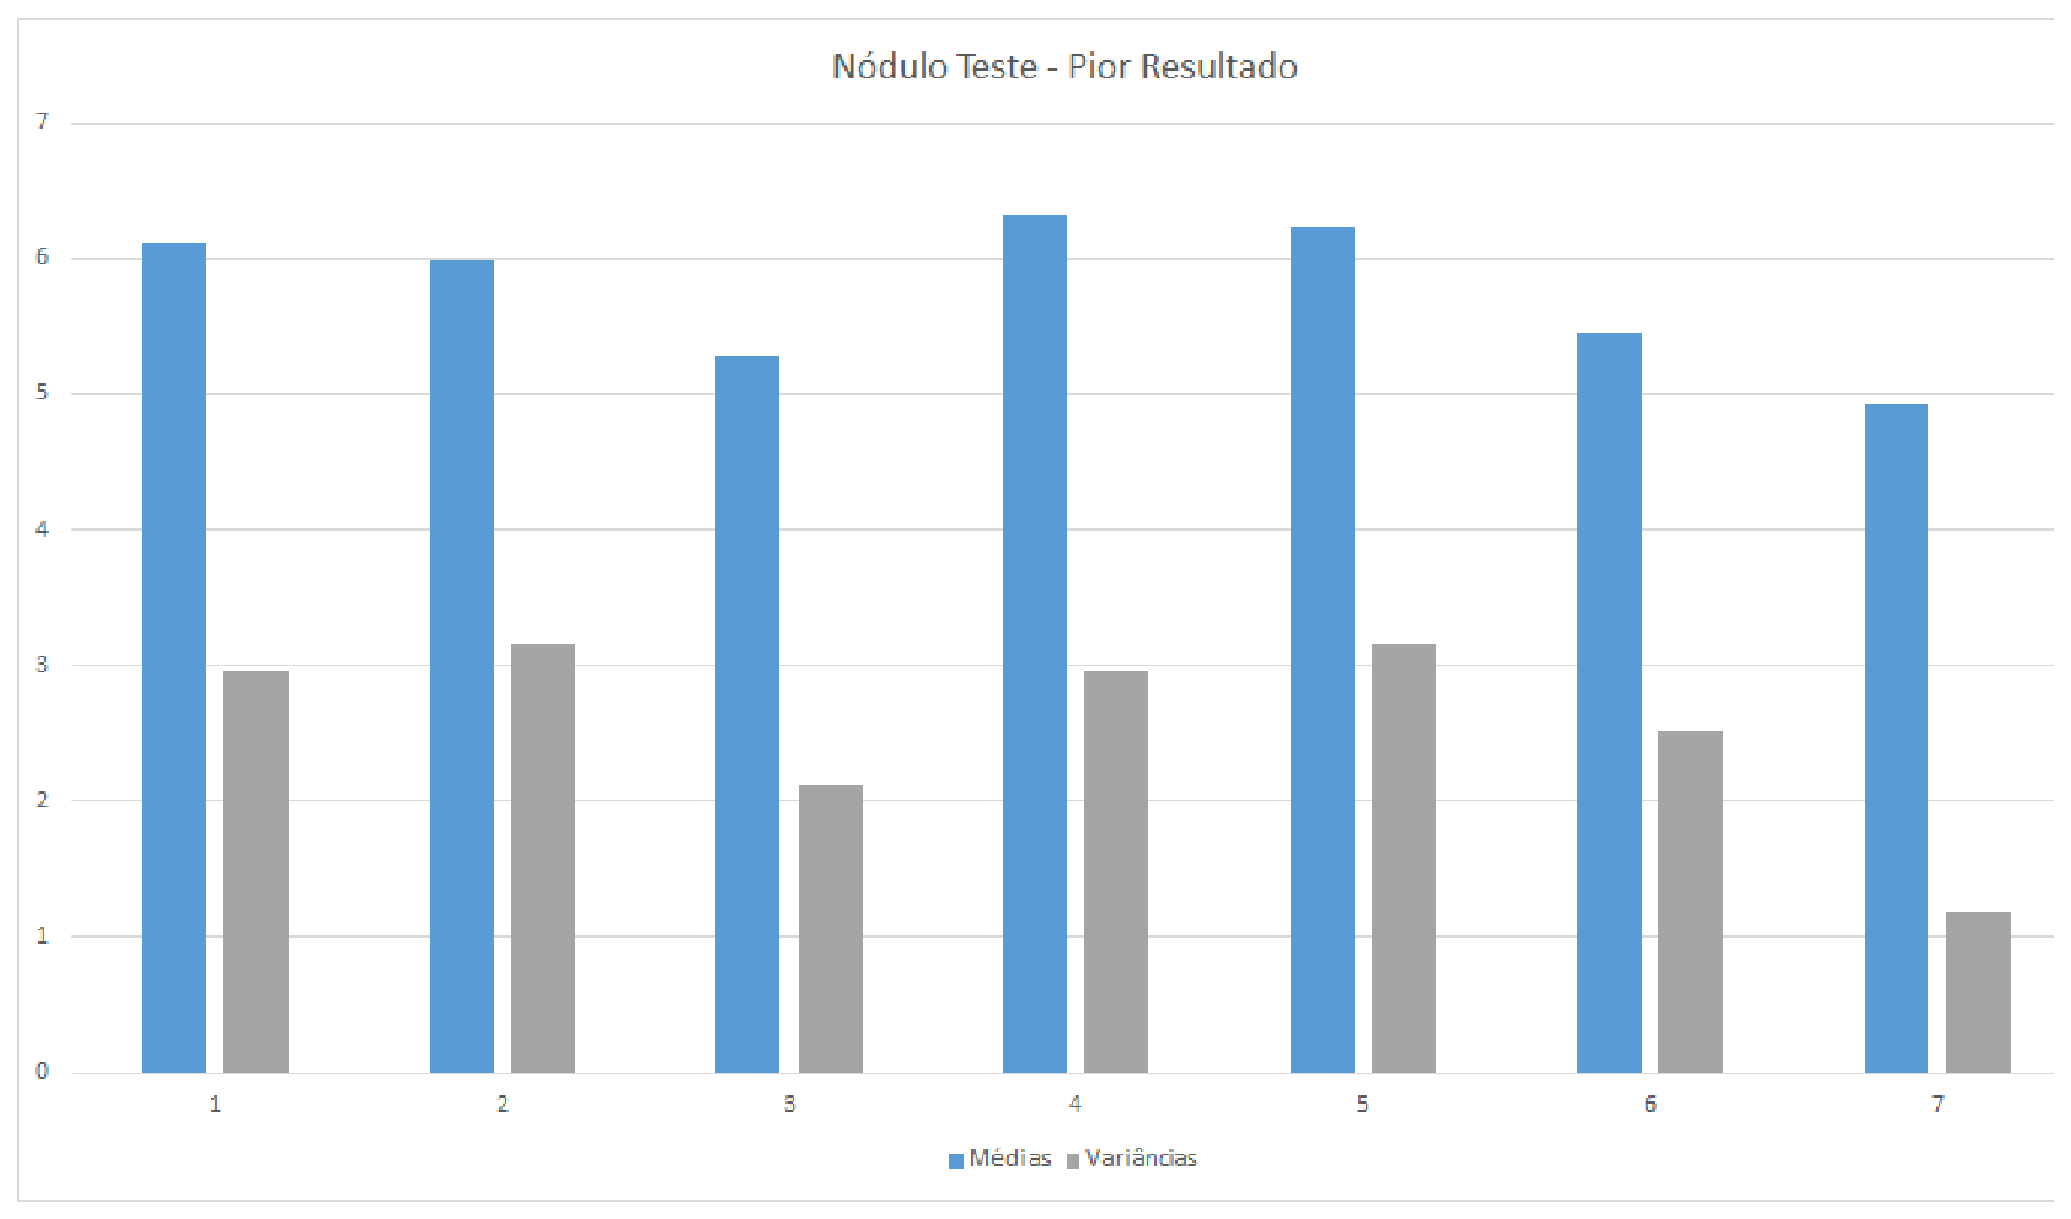
\includegraphics[width=0.70\hsize]{figuras_tcc/pior_resultado/nodulo_teste_pior.eps}
\caption{Valores dos sinais de pacientes com n\'{o}dulo, selecionados para o grupo teste, que geraram o pior resultado. }
\label{fig:nodulo_teste_pior}
\end{sidewaysfigure}
\begin{sidewaysfigure}
\centering
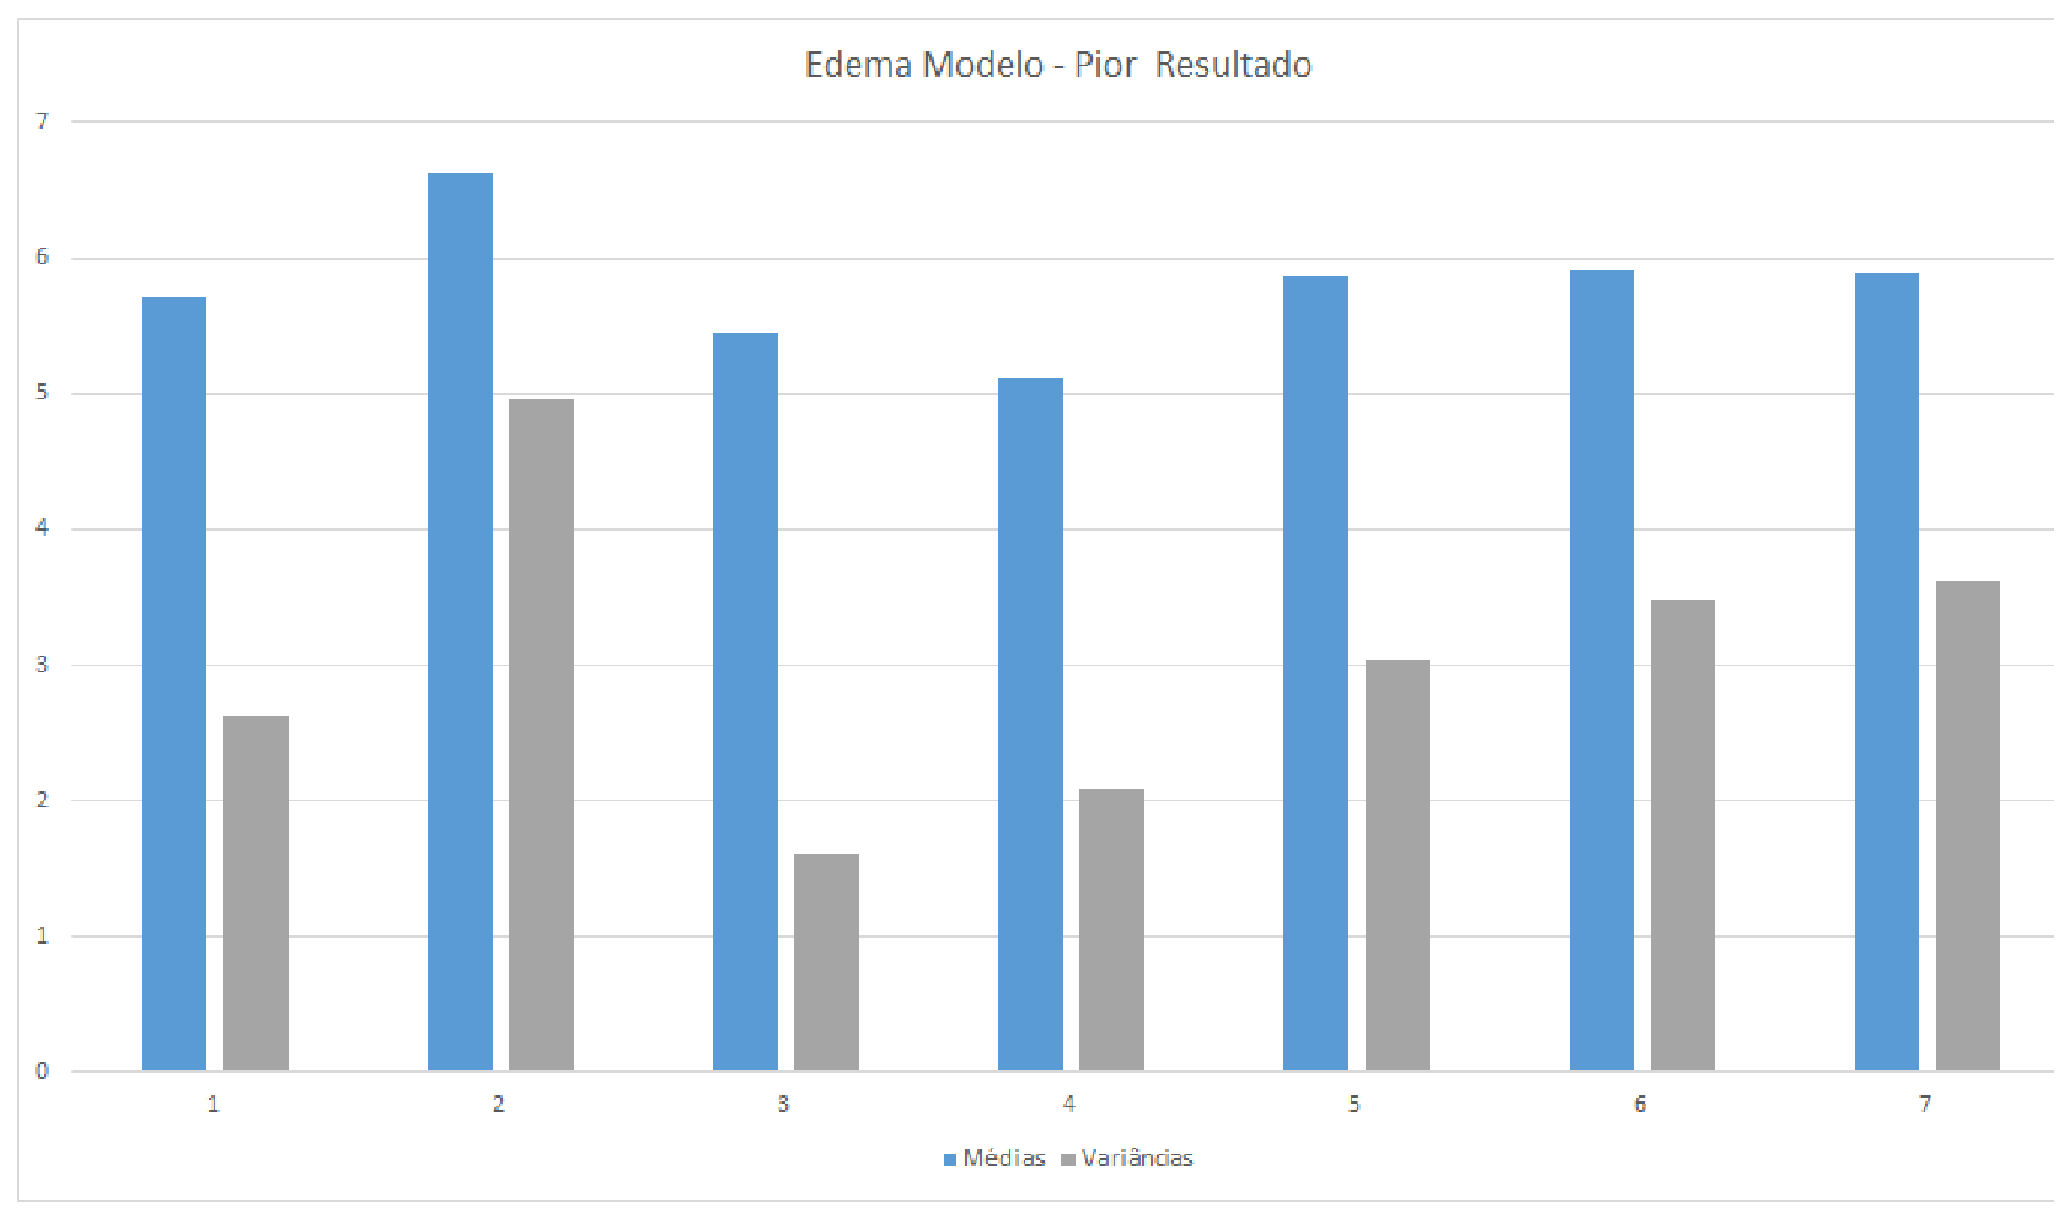
\includegraphics[width=0.70\hsize]{figuras_tcc/pior_resultado/edema_modelo_pior.eps}
\caption{Valores dos sinais de pacientes com edema, selecionados para o grupo modelo, que geraram o pior resultado. }
\label{fig:edema_modelo_pior}
\end{sidewaysfigure}
\begin{sidewaysfigure}
\centering
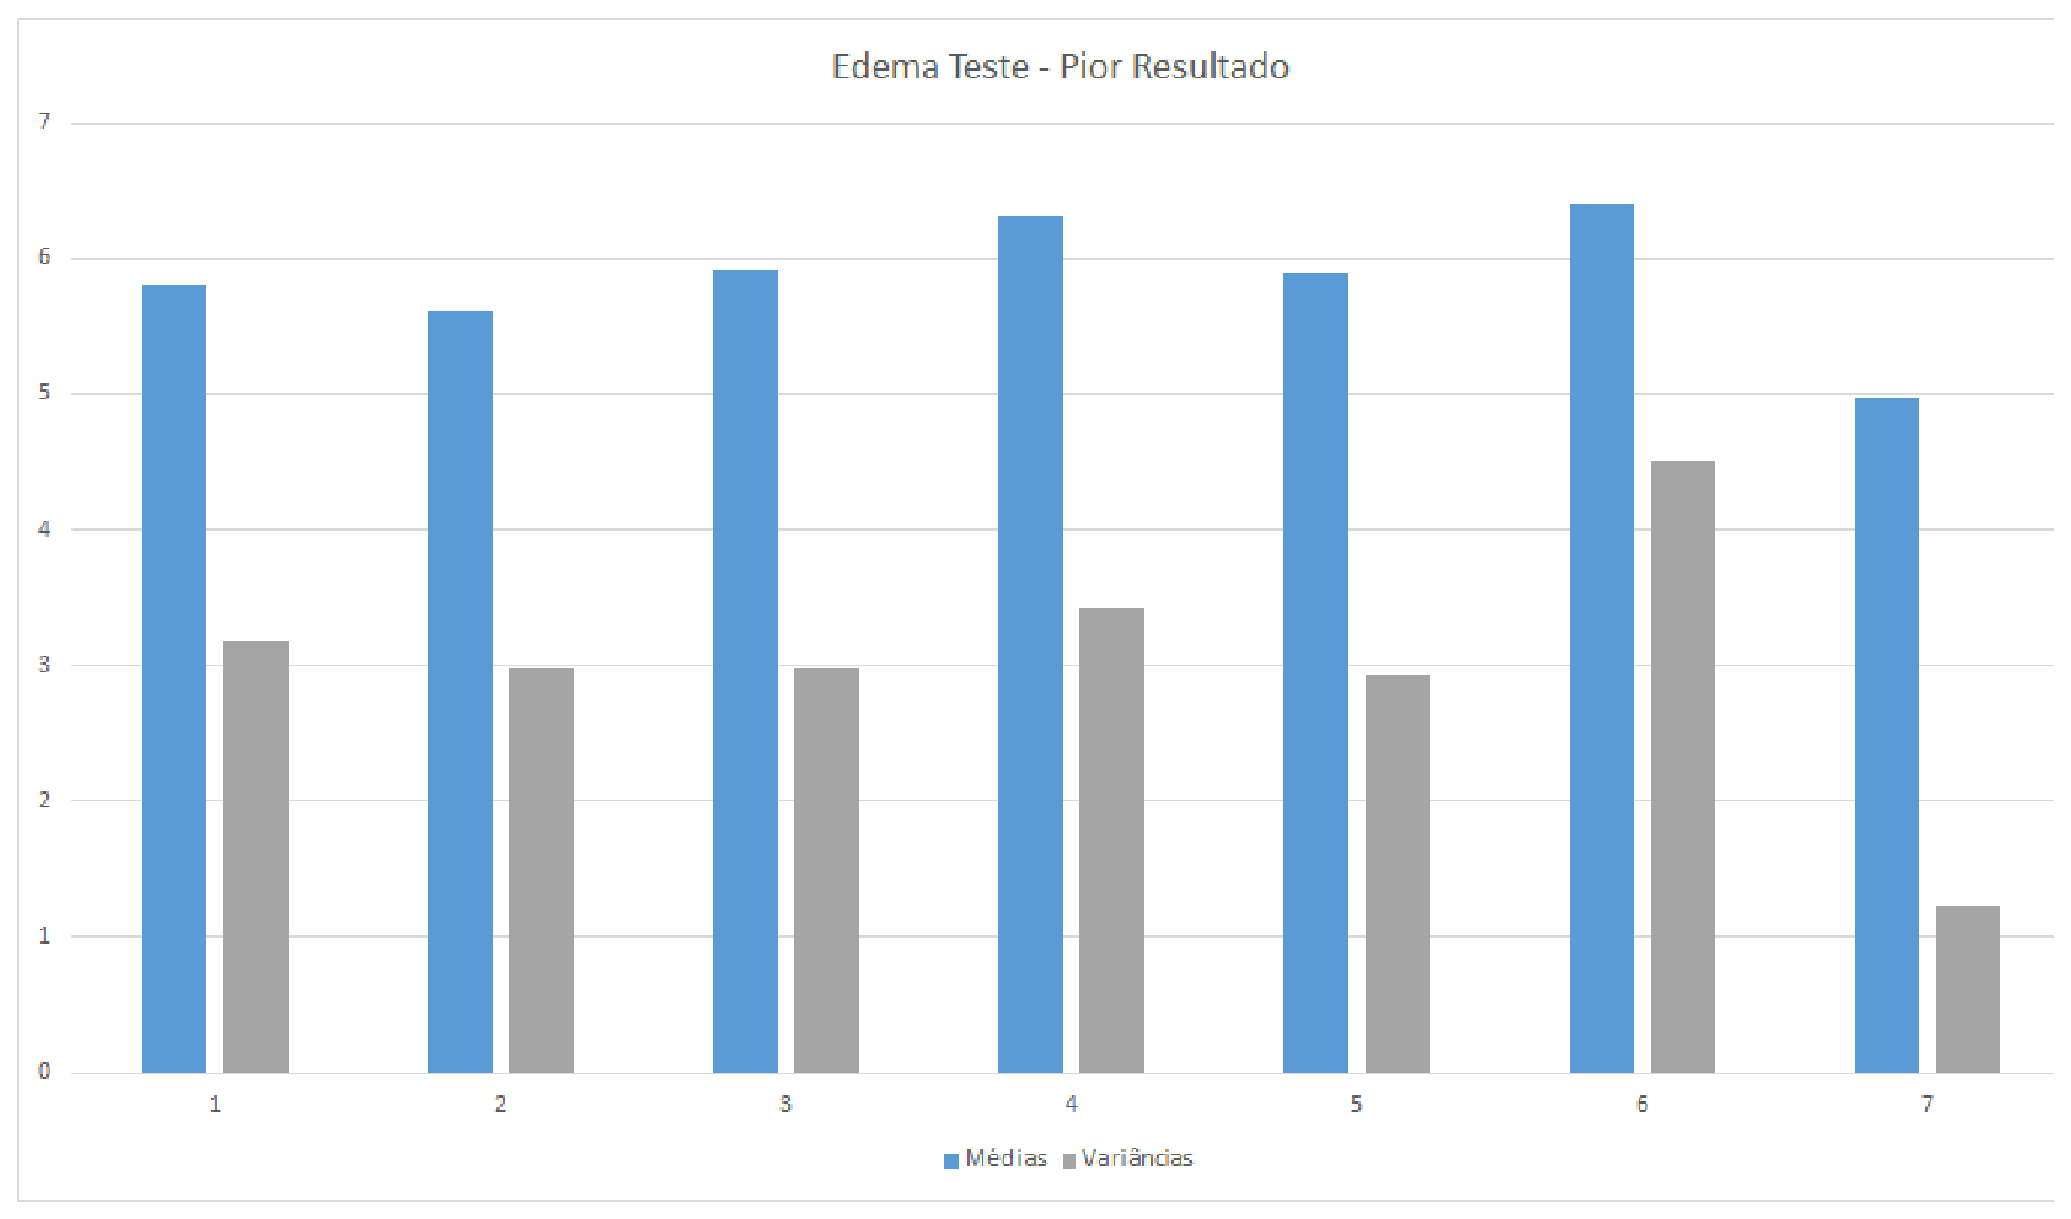
\includegraphics[width=0.70\hsize]{figuras_tcc/pior_resultado/edema_teste_pior.eps}
\caption{Valores dos sinais de pacientes com edema, selecionados para o grupo teste, que geraram o pior resultado. }
\label{fig:edema_teste_pior}
\end{sidewaysfigure}
\begin{sidewaysfigure}
\centering
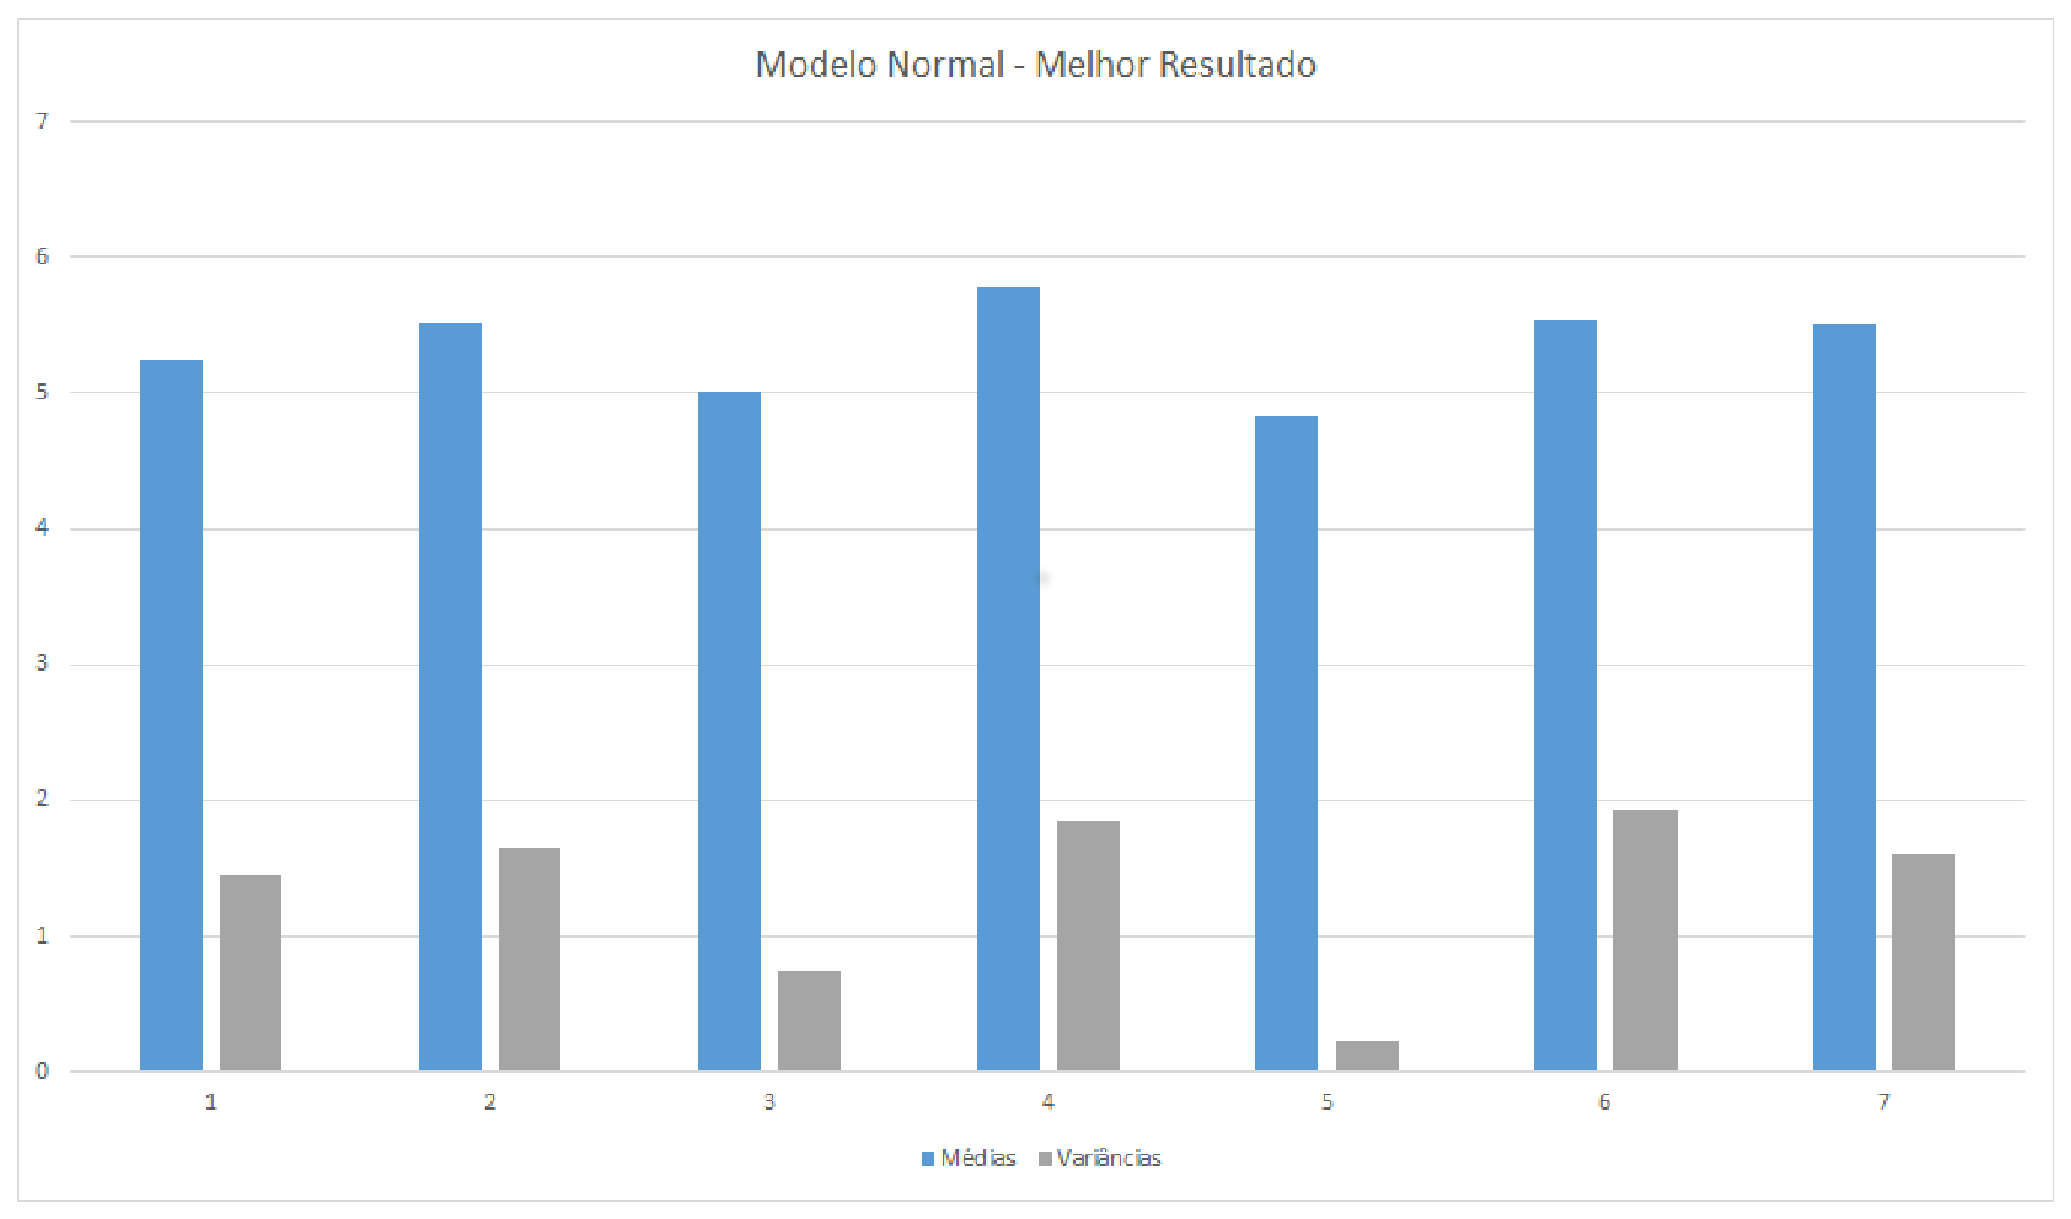
\includegraphics[width=0.70\hsize]{figuras_tcc/melhor_resultado/modelo_normal_melhor.eps}
\caption{Valores dos sinais de pacientes saud\'{a}veis, selecionados para o grupo modelo, que geraram o melhor resultado. }
\label{fig:normal_modelo_melhor}
\end{sidewaysfigure}
\begin{sidewaysfigure}
\centering
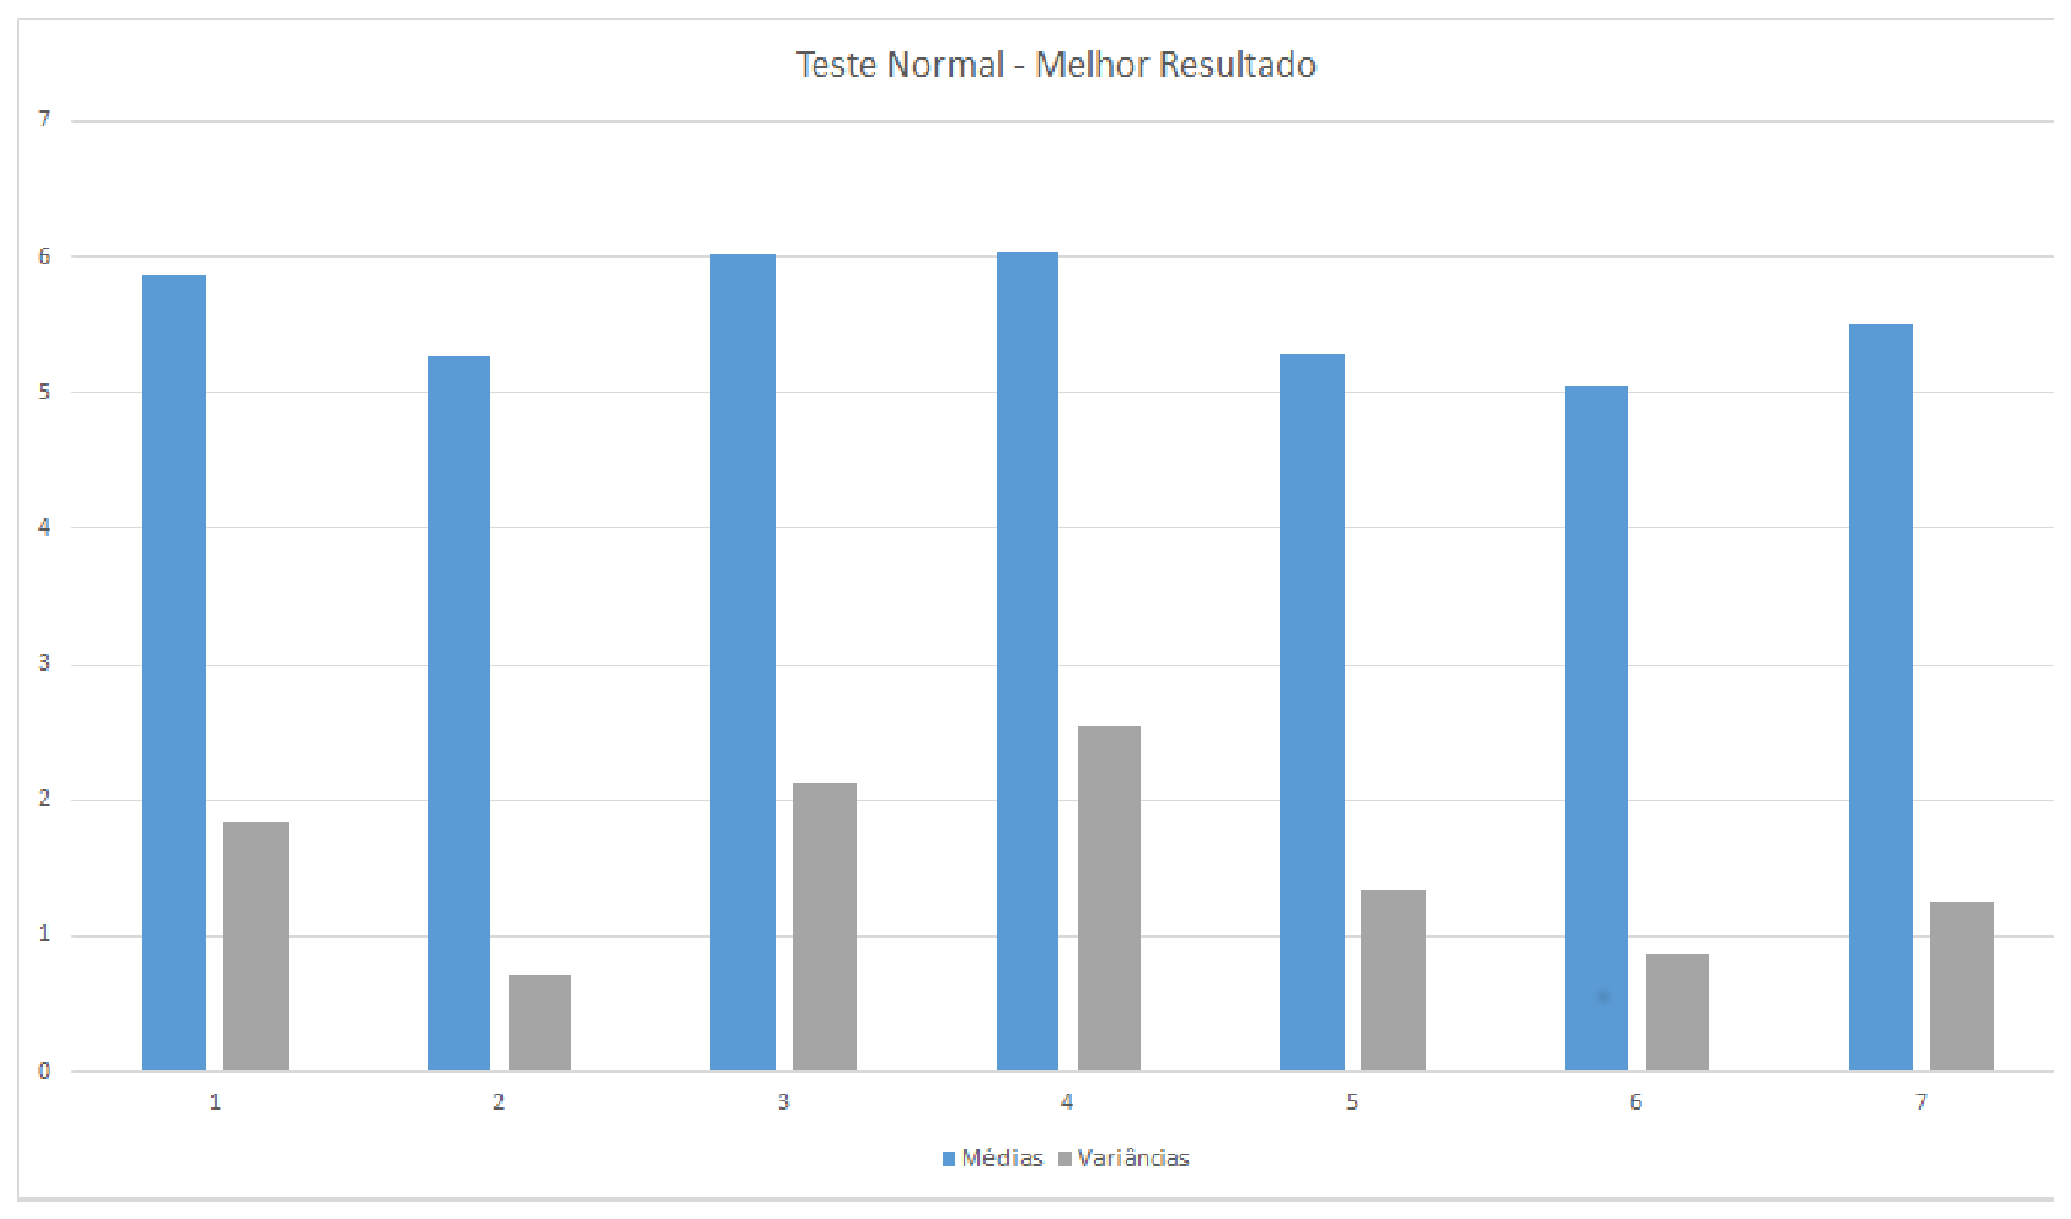
\includegraphics[width=0.70\hsize]{figuras_tcc/melhor_resultado/teste_normal_melhor.eps}
\caption{Valores dos sinais de pacientes saud\'{a}veis, selecionados para o grupo teste, que geraram o melhor resultado. }
\label{fig:normal_teste_melhor}
\end{sidewaysfigure}
\begin{sidewaysfigure}
\centering
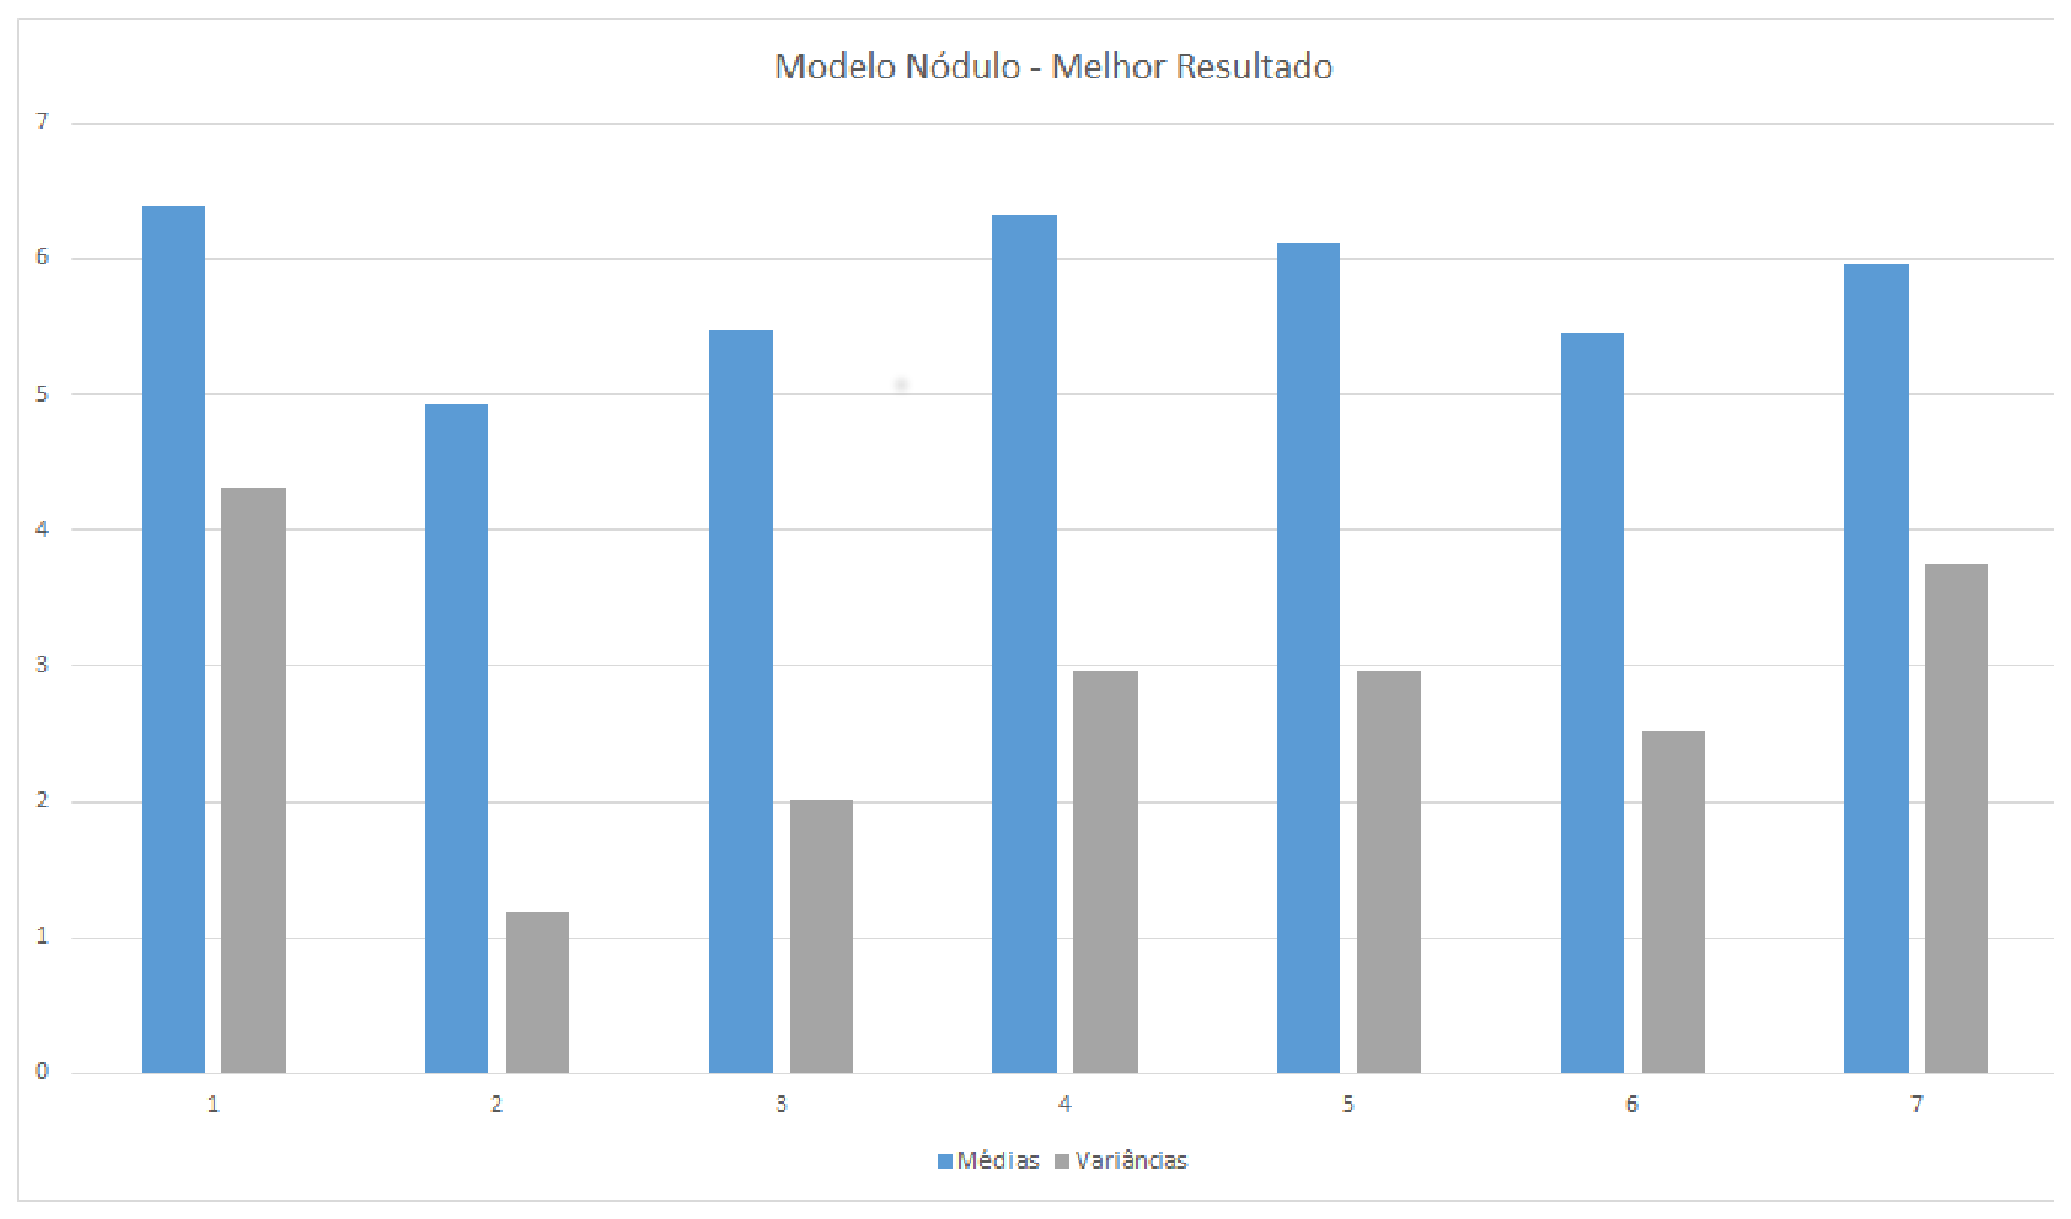
\includegraphics[width=0.70\hsize]{figuras_tcc/melhor_resultado/modelo_nodulo_melhor.eps}
\caption{Valores dos sinais de pacientes com no\'{o}dulo, selecionados para o grupo modelo, que geraram o melhor resultado. }
\label{fig:nodulo_modelo_melhor}
\end{sidewaysfigure}
\begin{sidewaysfigure}
\centering
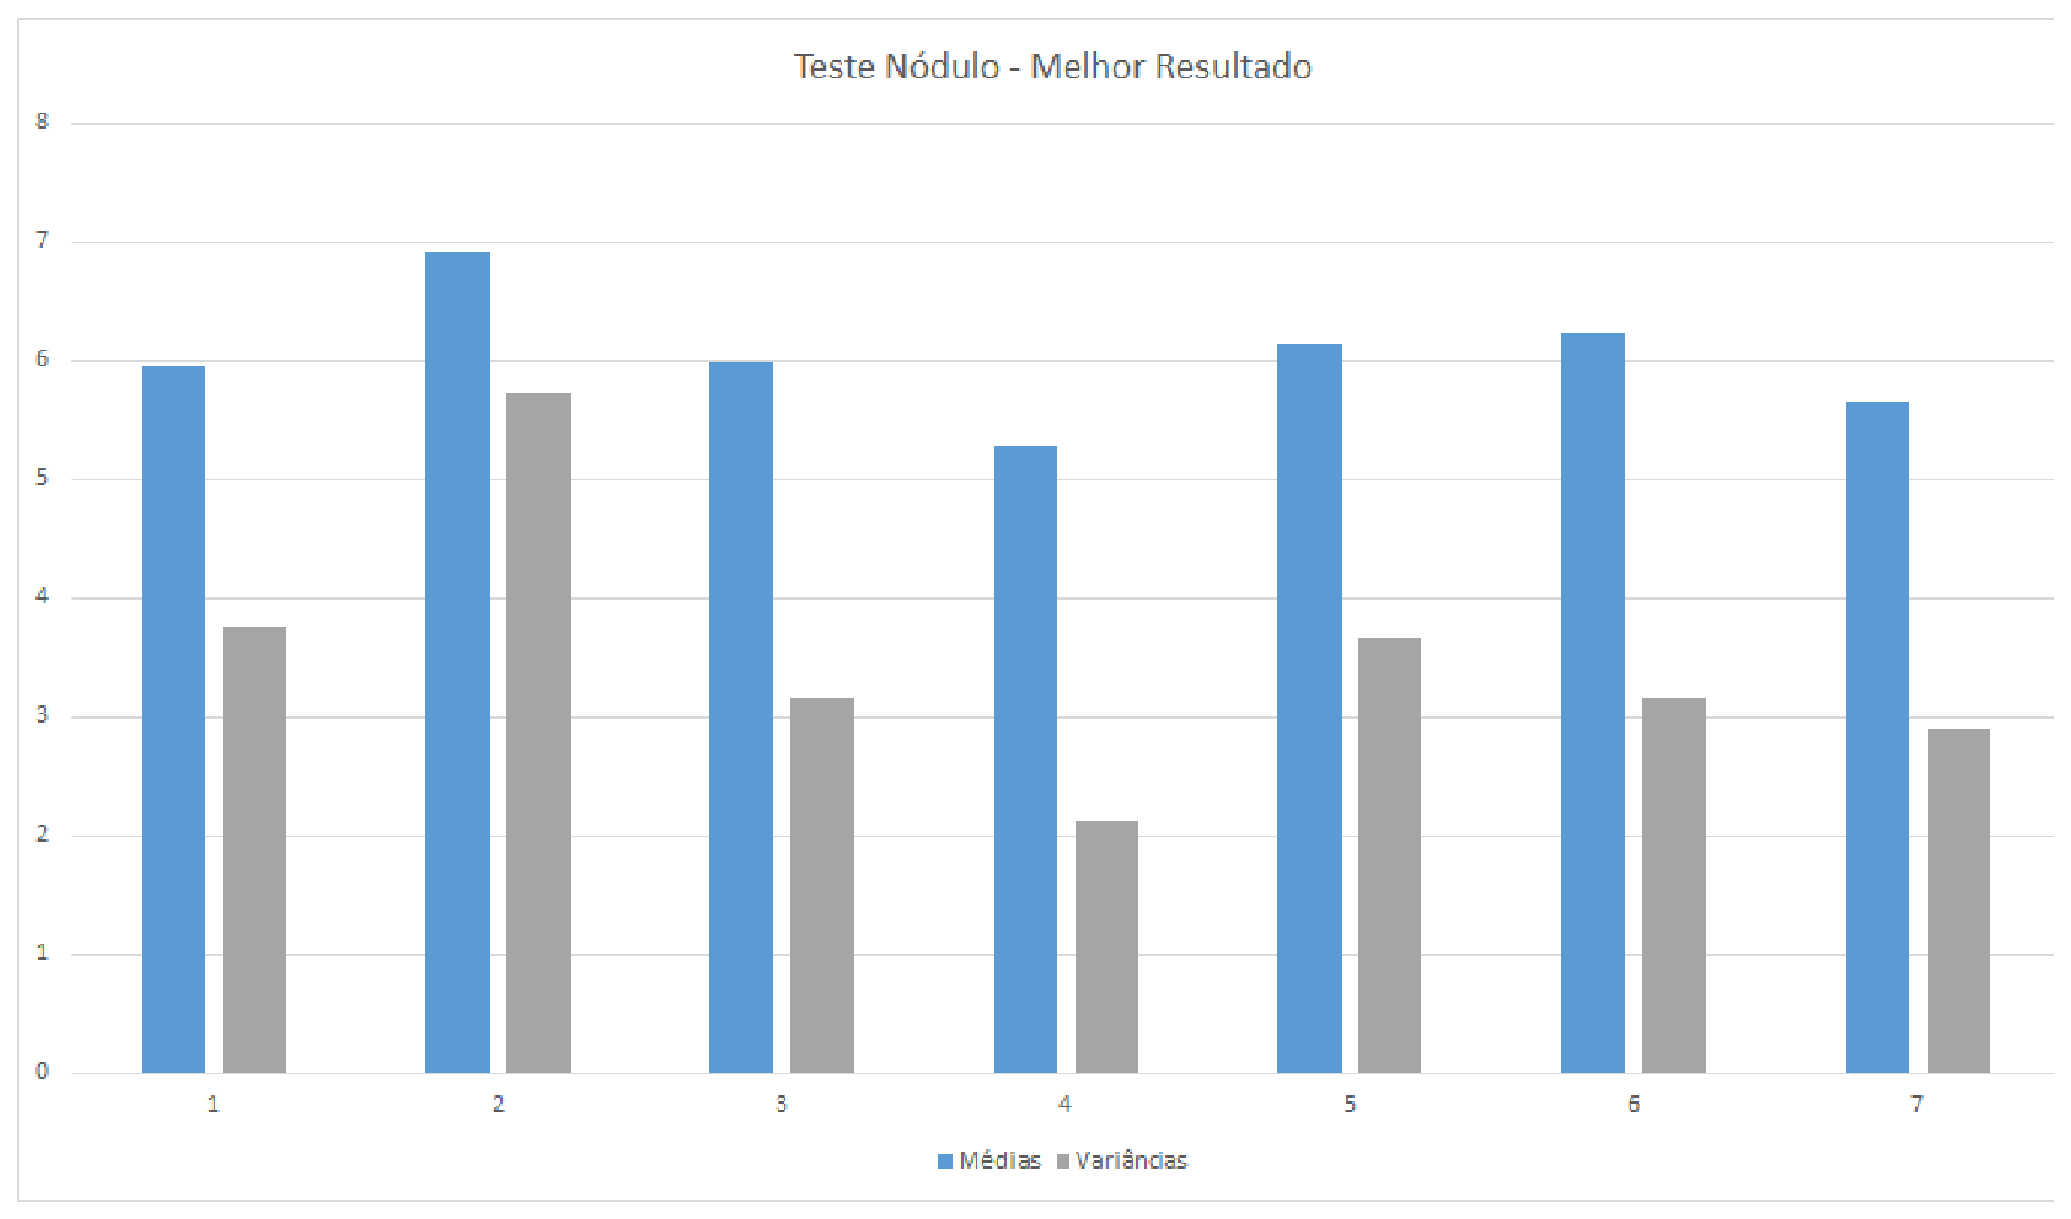
\includegraphics[width=0.70\hsize]{figuras_tcc/melhor_resultado/teste_nodulo_melhor.eps}
\caption{Valores dos sinais de pacientes com no\'{o}dulo, selecionados para o grupo teste, que geraram o melhor resultado. }
\label{fig:nodulo_teste_melhor}
\end{sidewaysfigure}
\begin{sidewaysfigure}
\centering
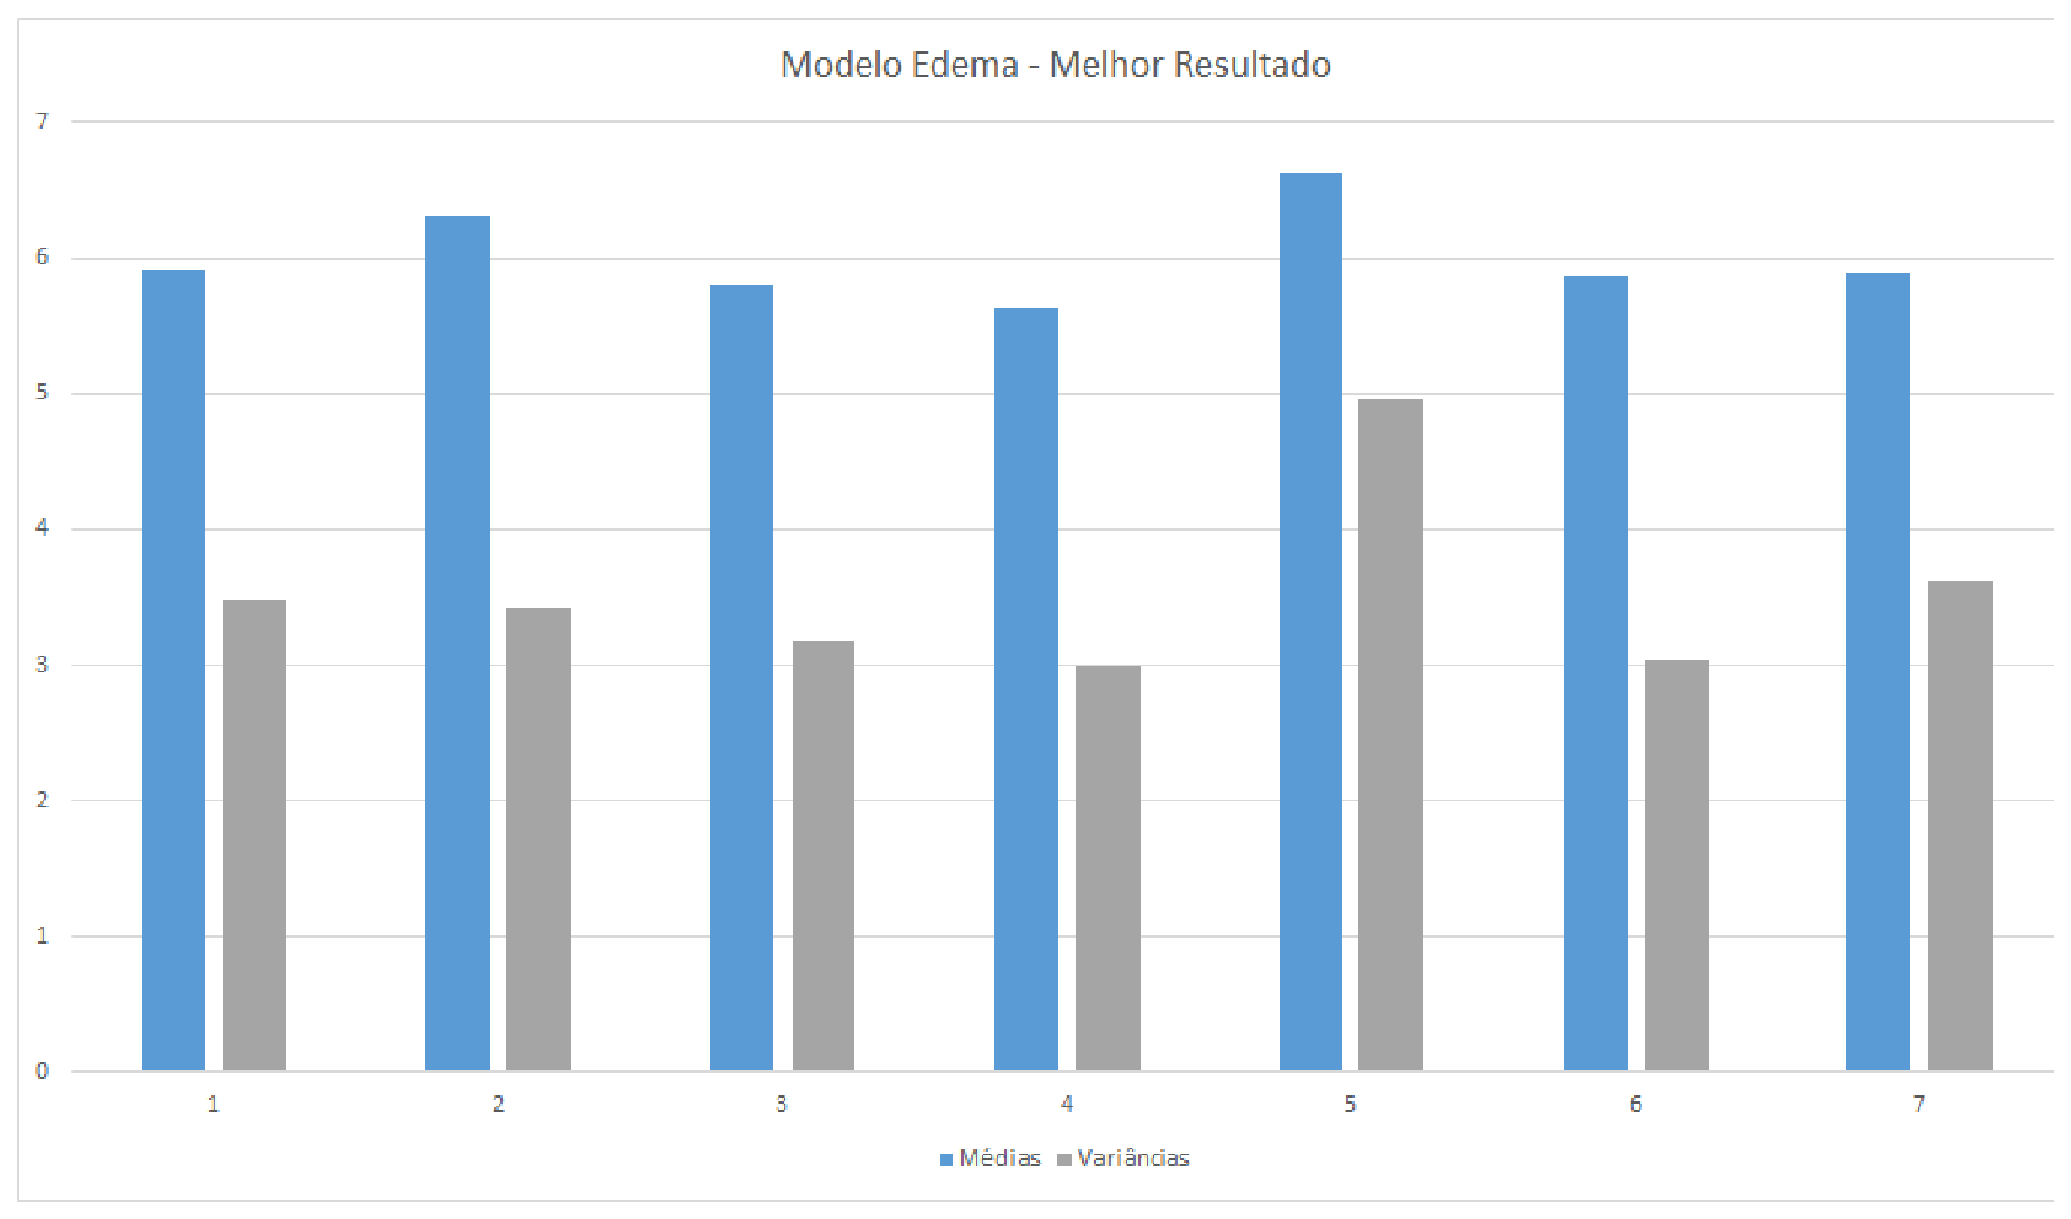
\includegraphics[width=0.70\hsize]{figuras_tcc/melhor_resultado/modelo_edema_melhor.eps}
\caption{Valores dos sinais de pacientes com edema, selecionados para o grupo modelo, que geraram o melhor resultado. }
\label{fig:edema_modelo_melhor}
\end{sidewaysfigure}
\begin{sidewaysfigure}
\centering
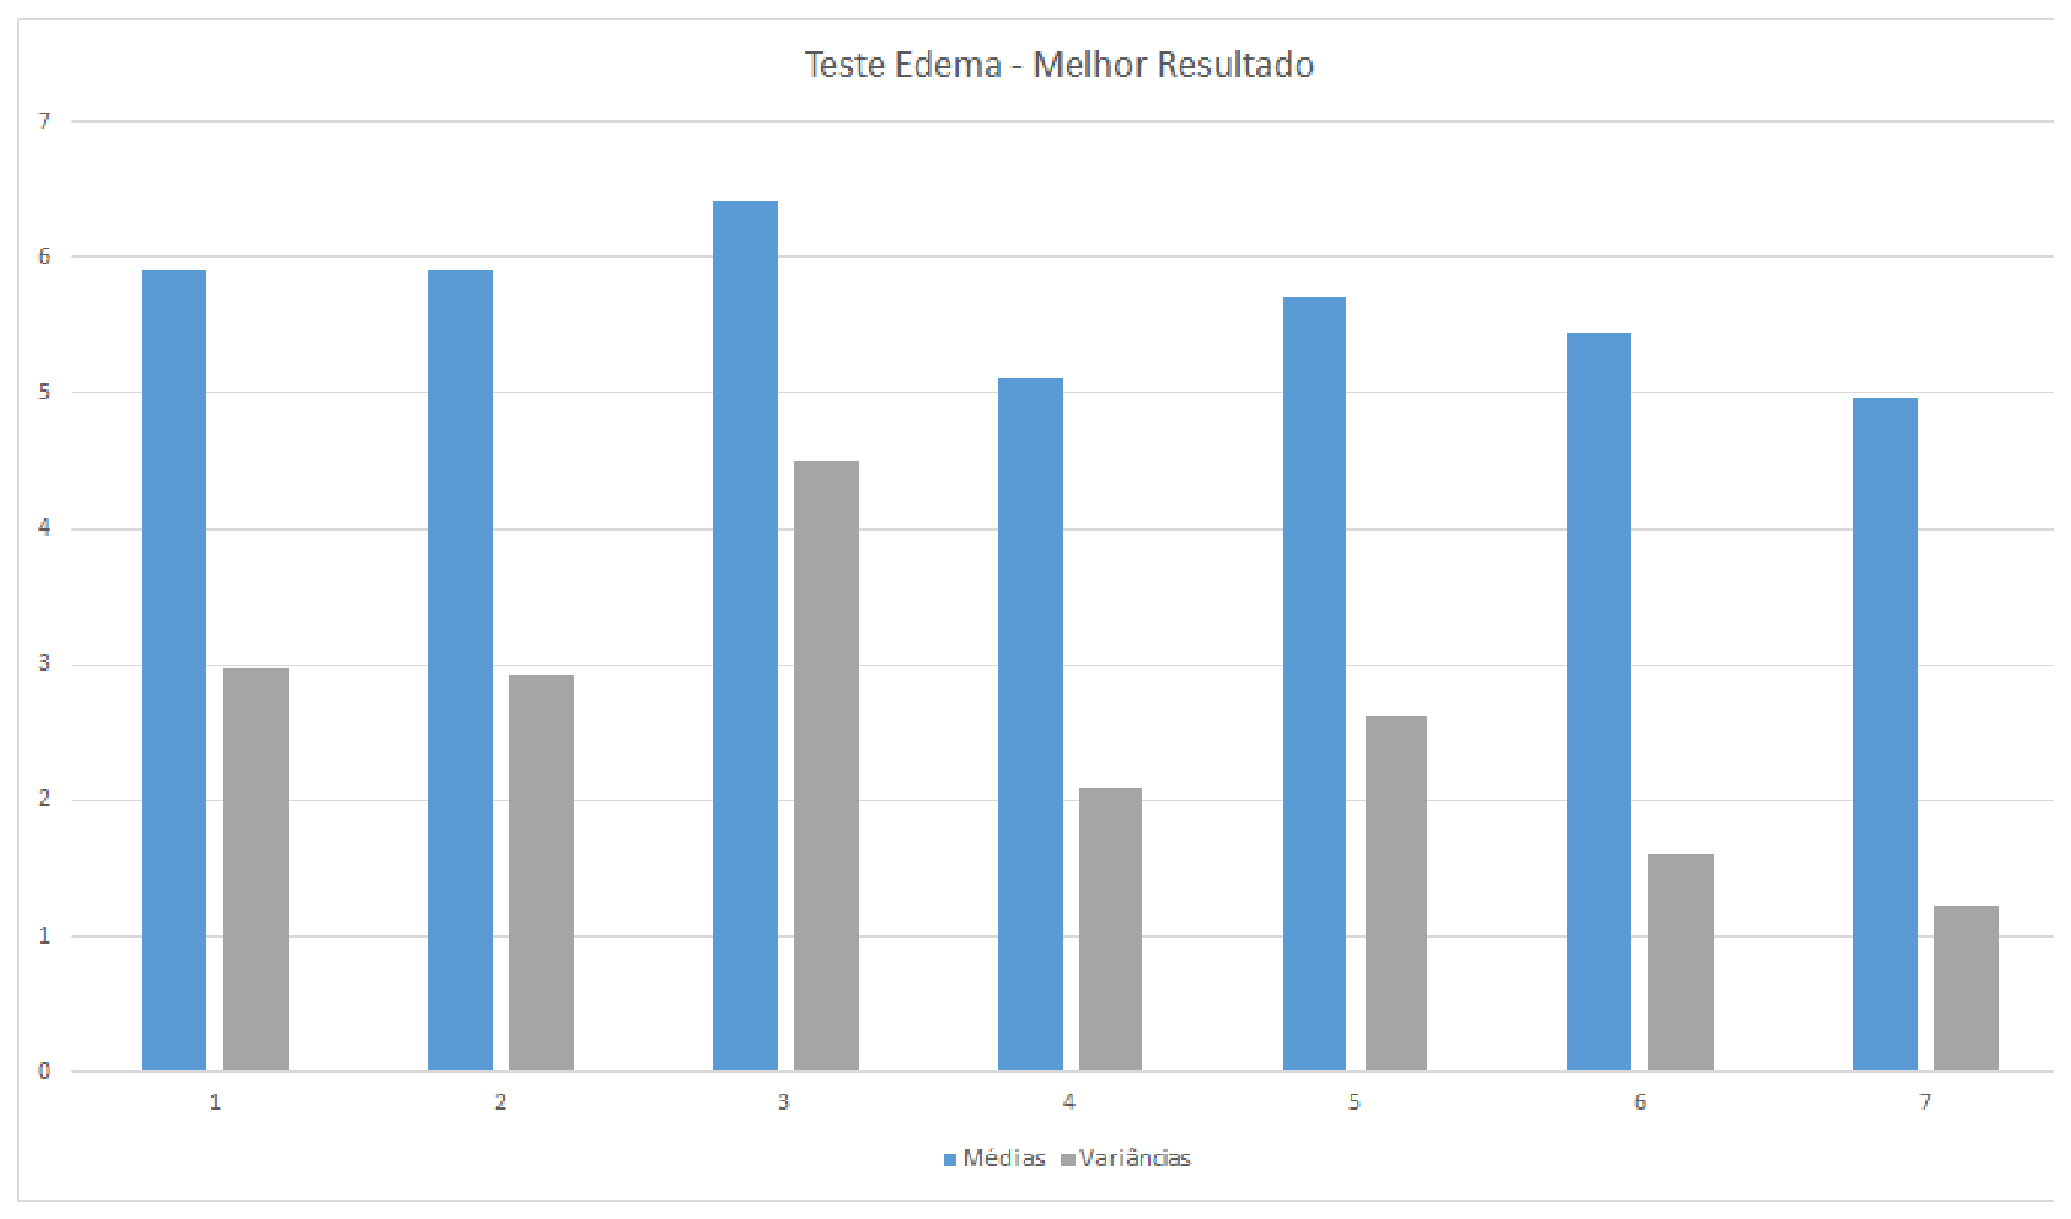
\includegraphics[width=0.70\hsize]{figuras_tcc/melhor_resultado/teste_edema_melhor.eps}
\caption{Valores dos sinais de pacientes com edema, selecionados para o grupo teste, que geraram o melhor resultado. }
\label{fig:edema_teste_melhor}
\end{sidewaysfigure}
\end{appendices}
%%%%%%%%%%%%%%%%%%%%%%%%%%%%%%%%%%%%%%%%%%%%%%%%%%%% pedaco retirado do cpt 2
%%//////////////////////////////////////////////////// bibliografia
\begin{thebibliography}{9}
\bibitem{costa_doutorado}W. C. d. A. Costa, ''An\'{a}lise din\^{a}mica n\~{a}o linear de sinais de voz para detec\c{c}\~{a}o de patologias lar\'{i}ngeas,''
Universidade Federal de Campina Grande. Tese de doutorado, 2012.
\bibitem{vieira_outros}V. Vieira, S. Costa, W. Costa, S. Correia, and F. Assis, ''Discrimina\c{c}\~{a}o de sinais de voz com an\'{a}lise de quantifica\c{c}\~{a}o de recorr\^{e}ncia e redes neurais mlp,'' XXXI Simp\'{o}sio Brasileiro de Telecomunica\c{c}\~{o}es (SBrT 2013), 2013.
\bibitem{souza_mestrado}Taciana A. Souza et al, Voice pathology assessment using wavelet based on texture analysis of recurrence plots, IFPB, Jo\~{a}o Pessoa, Brazil; em Telecommunications (IWT), 2015 International Workshop, 14-17 junho de 2015.  IEEE, DOI: 10.1109/IWT.2015.7224580.
\bibitem{arias_londono}J. D. Arias-Londono, J. I. Godino-Llorente, N. S\'{a}enz-Lech\'{o}n, V. Osma-Ruiz, and G. Castellanos-Dominguez, ''Automatic detection of pathological voices using complexity measures, noise parameters, and mel-cepstral coefficients,'' Biomedical Engineering, IEEE Transactions on, vol. 58, 2011.
\bibitem{livro_laringe_henrique}I. A. Kuhl, ''Laringologia Pr\'{a}tica Ilustrada'', Segunda Edi\c{c}\~{a}o, Editora Revinter, ISBN: 85-7309-121-5.
\bibitem{the_larynx}M. P. Fried, ''The Larynx: A Multidisciplinary Approach'', Segunda Edi\c{c}\~{a}o, ISBN: 978-0801680465.
\bibitem{definicao_taxa_amostragem1}C. E. Shannon, ''Comunication in the presence of noise,'' Proc. IRE, vol. 37, no. 1, pp. 10–21, Jan. 1949.
\bibitem{definicao_taxa_amostragem2}C. E. Shannon, ''Comunication in the presence of noise,'' Proc. IEEE, vol. 72, no. 9, pp. 1192–1201, Sep. 1984.
\bibitem{livro_estatistica}W. d. O. Bussab, P. A. Morettin, Estat\'{i}stica B\'{a}sica - 8 Ed. 2013.
\bibitem{formato_wave_completo}Issued as a joint design by IBM Corporation and Microsoft Corporation, \enquote{Multimedia Programming Interface and Data Specification v1.0}
\bibitem{referencia_matriz_confusao}S. Visa, B. Ramsay, A. Ralescu, E. v. d. Knaap, \enquote{Confusion Matrix-based Feature Selection}, confer\^{e}ncia \enquote{Midwest Artificial Intelligence and Cognitive Science}, 2011, Cincinnati, USA, April 16-17.
\bibitem{distancia_euclidiana}E. Deza, M. M. Deza, \enquote{Encyclopedia of Distances}, editora Springer, p. 94, 2009.
\bibitem{godino} Godino-Llorente JI, Gomes-Vilda P, Blanco-Velasco M. Dimensionality reduction of a pathological voice quality assessment system based on gaussian mixture models and short-term cepstral parameters. IEEE Transactions on Biomedical Engineering. 2006; 53(10):1943-1953. 
\bibitem{wang}Wang X, Zhang J, Yan Y. Discrimination between pathological and normal voices using GMM-SVM approach. Journal of Voice. 2011; 25(1):38-43
\bibitem{figura_wave}C. S. Sapp  WAVE PCM soundfile format, dispon\'{i}vel em: http://soundfile.sapp.org/doc/WaveFormat/wav-sound-format.gif
\bibitem{wca_costa}Costa WCA, Vieira VJD, Costa SC, Assis FM, Aguiar Neto BG. Avalia\c{c}\~{a}o do uso combinado de medidas de quantifica\c{c}\~{a}o de recorrência e an\'{a}lise LPC na classifica\c{c}\~{a}o de vozes patol\'{o}gicas. In: Anais do XXIII Congresso Brasileiro de Engenharia Biom\'{e}dica (CBEB 2012); Porto de Galinhas, Brasil. 2012
\bibitem{melcepstral}L. R. Rabiner and B. H. Juang, Fundamentals of Speech Recognition. Englewood Cliffs, NJ: Prentice-Hall, 1993
\bibitem{henriquez}Henr\'{i}quez P, Alonso JB, Ferrer MA, Travieso CM, Godino-Llorente, D\'{i}az-de-Mar\'{i}a F. Characterization of healthy and pathological voice through measures based on nonlinear dynamics. IEEE Transactions on Audio, Speech and Language Processing. 2009; 17(6):1186-1195
\bibitem{boyanov}B. Boyanov and S. Hadjitodorov, ''Acoustic analysis of pathological voices: A voice analysis system for screening of laryngeal diseases,'' IEEE Eng. Med. Biol. Mag., vol. 16, pp. 74–82, Jul./Aug. 1997.
\bibitem{calc_numerico}M.A. Gomes Ruggiero, V. L. da Rocha Lopes. C\'{a}lculo Num\'{e}rico - Aspectos Te\'{o}ricos e Computacionais, 2ª edi\c{c}\~{a}o, Editora Pearson, 1997.
\end{thebibliography}
\end{document}